\documentclass[12pt,a4paper]{article}
\usepackage[utf8]{inputenc}
\usepackage[margin=1in]{geometry}
\usepackage{amsmath}
\usepackage{amssymb}
\usepackage{graphicx}
\usepackage{tikz}
\usepackage{enumitem}
\usepackage{xcolor}
\usepackage{tcolorbox}
\usepackage{fancyhdr}
\usepackage{hyperref}
\usepackage{pifont}
\usepackage{mdframed}
\usepackage{tcolorbox}
\tcbuselibrary{breakable}

\newcommand{\cmark}{\ding{51}} 
\newcommand{\xmark}{\ding{55}} 


\usetikzlibrary{shapes.geometric, arrows, positioning, er}

% Custom boxes for important concepts
\newtcolorbox{intuition}{
  colback=blue!5!white,
  colframe=blue!75!black,
  title=Intuition,
  breakable
}

\newtcolorbox{example}{
  colback=green!5!white,
  colframe=green!75!black,
  title=Example,
  breakable
}

\newtcolorbox{key}{
  colback=yellow!10!white,
  colframe=orange!75!black,
  title=Key Concept,
  breakable
}

\newtcolorbox{warning}{
  colback=red!5!white,
  colframe=red!75!black,
  title=Common Mistake,
  breakable
}

\pagestyle{fancy}
\fancyhf{}

\rhead{DBMS \& Data Warehousing}

\rfoot{Page \thepage}

\setlength{\headheight}{15pt}
\renewcommand{\headrulewidth}{0.4pt}
\renewcommand{\footrulewidth}{0pt}

\title{\textbf{Database Management and Data Warehousing}}
\author{Comprehensive Notes}
\date{}

\begin{document}

\maketitle
\tableofcontents
\newpage

\section{Introduction: Why Do We Need Databases?}

\begin{intuition}
Imagine you're running a university. You have students, courses, professors, classrooms, grades, schedules. How do you organize all this information?

You could use:
\begin{itemize}
    \item \textbf{Paper files}: Hard to search, easy to lose, difficult to update
    \item \textbf{Excel sheets}: Better, but what if two people update simultaneously? What if you need to find "all students who took courses taught by Prof. Smith"?
    \item \textbf{A database}: Organized, searchable, handles concurrent access, maintains relationships
\end{itemize}

The ER Model is our \textit{blueprint} - like an architect's drawing before building a house. It helps us design how data should be organized \textbf{before} we build the actual database.
\end{intuition}

\subsection{What is a Database?}

A database is a \textbf{structured collection of related data} with these properties:

\begin{enumerate}
    \item \textbf{Persistent}: Data survives after the program ends
    \item \textbf{Shared}: Multiple users can access simultaneously
    \item \textbf{Consistent}: Data follows rules (e.g., a student can't enroll in a course that doesn't exist)
    \item \textbf{Secure}: Only authorized users can access certain data
\end{enumerate}

\subsection{The Design Process}

Think of database design like building a house:

\begin{center}
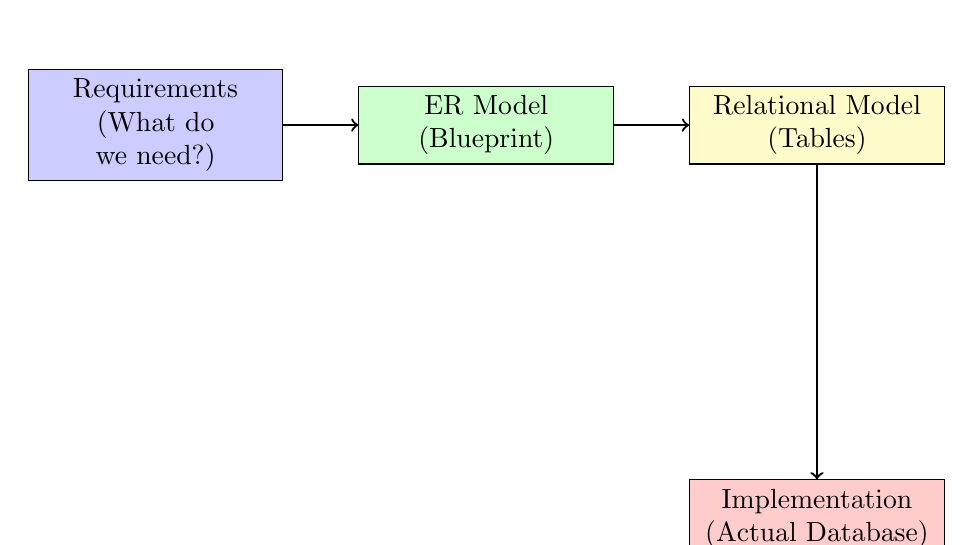
\begin{tikzpicture}[
    node distance=4.2cm,
    every node/.style={rectangle, draw, text width=3cm, align=center}
]

\node (req) [fill=blue!20] {Requirements\\(What do we need?)};
\node (er)  [fill=green!20, right of=req] {ER Model\\(Blueprint)};
\node (rel) [fill=yellow!20, right of=er] {Relational Model\\(Tables)};
\node (impl)[fill=red!20, below of=rel, yshift=-0.8cm] {Implementation\\(Actual Database)};

\draw [->, thick] (req) -- (er);
\draw [->, thick] (er) -- (rel);
\draw [->, thick] (rel) -- (impl);

\end{tikzpicture}
\end{center}

We're focusing on the \textbf{ER Model} in this chapter - the conceptual blueprint.

\section{Core Building Blocks of ER Model}

\begin{key}
The ER Model has THREE fundamental components:
\begin{enumerate}
    \item \textbf{Entities}: Things that exist (nouns)
    \item \textbf{Attributes}: Properties of things (adjectives)
    \item \textbf{Relationships}: Connections between things (verbs)
\end{enumerate}
\end{key}

\subsection{Entities: The "Things" in Your World}

\begin{intuition}
An entity is anything you want to store information about. Ask yourself: "What are the important \textit{things} in my system?"

For a university:
\begin{itemize}
    \item Student (a thing)
    \item Course (a thing)
    \item Professor (a thing)
    \item Department (a thing)
\end{itemize}

For a hospital:
\begin{itemize}
    \item Patient, Doctor, Medicine, Appointment
\end{itemize}

An entity is NOT a specific instance. "Student" is an entity type. "John Smith, ID: 12345" is an entity instance.
\end{intuition}

\textbf{Notation:} Entities are represented by rectangles.

\begin{center}
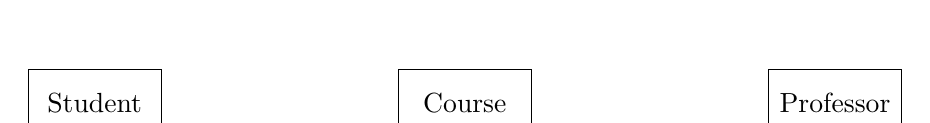
\begin{tikzpicture}
\node[entity] (student) {Student};
\node[entity, right=3cm of student] (course) {Course};
\node[entity, right=3cm of course] (professor) {Professor};
\end{tikzpicture}
\end{center}

\subsection{Attributes: Properties of Entities}

\begin{intuition}
Attributes answer: "What do I need to know about this thing?"

For a \textbf{Student} entity:
\begin{itemize}
    \item Student\_ID (unique identifier)
    \item Name
    \item Date\_of\_Birth
    \item Email
    \item Phone\_Number
\end{itemize}

Think of attributes as the columns you'd want in a table about students.
\end{intuition}

\subsubsection{Types of Attributes}

\textbf{1. Simple vs. Composite Attributes}

\begin{example}
\textbf{Simple}: Cannot be divided further
\begin{itemize}
    \item Age: 20
    \item Student\_ID: 12345
\end{itemize}

\textbf{Composite}: Can be broken down into smaller parts
\begin{itemize}
    \item Name $\rightarrow$ \{First\_Name, Middle\_Name, Last\_Name\}
    \item Address $\rightarrow$ \{Street, City, State, ZIP\_Code\}
\end{itemize}

Why does this matter? If you might want to search by last name only, make Name composite. If you'll always use the full name, keep it simple.
\end{example}

\textbf{2. Single-Valued vs. Multi-Valued Attributes}

\begin{example}
\textbf{Single-Valued}: One value per entity instance
\begin{itemize}
    \item Date\_of\_Birth: "1995-05-15" (a person has one birth date)
    \item Student\_ID: "12345" (one ID per student)
\end{itemize}

\textbf{Multi-Valued}: Can have multiple values
\begin{itemize}
    \item Phone\_Numbers: \{"555-1234", "555-5678"\} (a student might have home and mobile)
    \item Skills: \{"Python", "SQL", "Machine Learning"\}
\end{itemize}

Notation: Multi-valued attributes shown with double ellipse.
\end{example}

\textbf{3. Stored vs. Derived Attributes}

\begin{example}
\textbf{Stored}: Directly stored in database
\begin{itemize}
    \item Date\_of\_Birth: "1995-05-15"
\end{itemize}

\textbf{Derived}: Calculated from other attributes
\begin{itemize}
    \item Age: Can be calculated from Date\_of\_Birth and current date
    \item Total\_Credits: Sum of credits from all courses taken
\end{itemize}

Why distinguish? Derived attributes save storage space and stay automatically updated, but stored attributes are faster to access.

Notation: Derived attributes shown with dashed ellipse.
\end{example}

\textbf{4. Key Attributes (Most Important!)}

\begin{key}
A \textbf{key attribute} uniquely identifies each entity instance.

Properties of a good key:
\begin{enumerate}
    \item \textbf{Unique}: No two entities have the same value
    \item \textbf{Minimal}: Remove any part and it's no longer unique
    \item \textbf{Non-null}: Must always have a value
    \item \textbf{Stable}: Shouldn't change over time
\end{enumerate}
\end{key}

\begin{example}
For Student entity:
\begin{itemize}
    \item \textcolor{green}{\textbf{Good key}}: Student\_ID (unique, stable, always exists)
    \item \textcolor{red}{\textbf{Bad key}}: Email (might change if student changes email)
    \item \textcolor{red}{\textbf{Bad key}}: Name (not unique - two students could have same name)
\end{itemize}

Notation: Key attributes are \underline{underlined}.
\end{example}

\subsubsection{Visual Representation}

\begin{center}
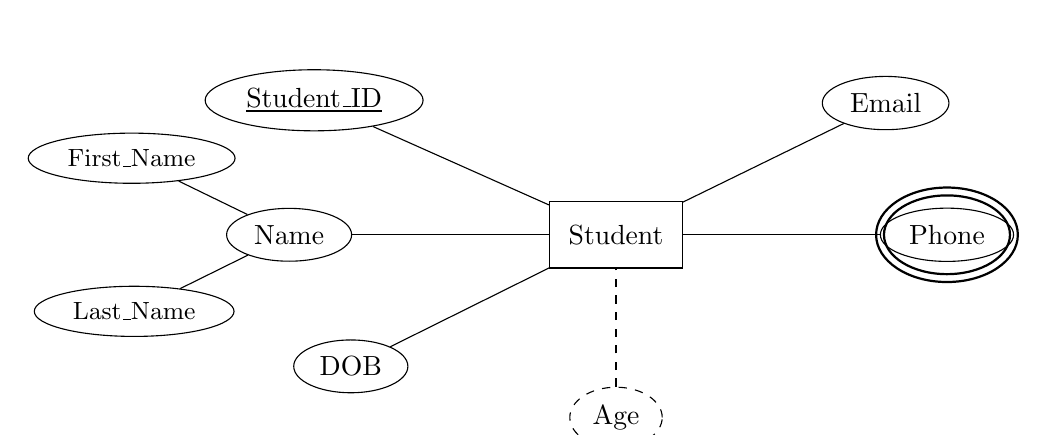
\begin{tikzpicture}[node distance=2cm]
% Entity
\node[entity] (student) {Student};

% Simple attributes
\node[attribute, above left=1cm and 2cm of student] (id) {\underline{Student\_ID}} edge (student);
\node[attribute, above right=1cm and 2cm of student] (email) {Email} edge (student);

% Composite attribute
\node[attribute, left=2.5cm of student] (name) {Name} edge (student);
\node[attribute, above left=0.5cm and 0.5cm of name, font=\small] (fname) {First\_Name} edge (name);
\node[attribute, below left=0.5cm and 0.5cm of name, font=\small] (lname) {Last\_Name} edge (name);

% Multi-valued attribute (double ellipse)
\node[attribute, right=2.5cm of student] (phone) {Phone} edge (student);
\draw[thick] (phone) ellipse (0.8cm and 0.5cm);
\draw[thick] (phone) ellipse (0.9cm and 0.6cm);

% Derived attribute (dashed)
\node[attribute, below=1.5cm of student, dashed, draw] (age) {Age} edge[dashed] (student);
\node[attribute, below left=1cm and 2cm of student] (dob) {DOB} edge (student);
\end{tikzpicture}
\end{center}

\subsection{Relationships: Connecting Entities}

\begin{intuition}
Relationships capture how entities interact.

Think verbs: Students \textit{enroll in} Courses. Professors \textit{teach} Courses. Patients \textit{visit} Doctors.

A relationship is NOT just "Student and Course are related." It's specifically "Student \textbf{enrolls in} Course."
\end{intuition}

\textbf{Notation:} Relationships are represented by diamonds.

\begin{center}
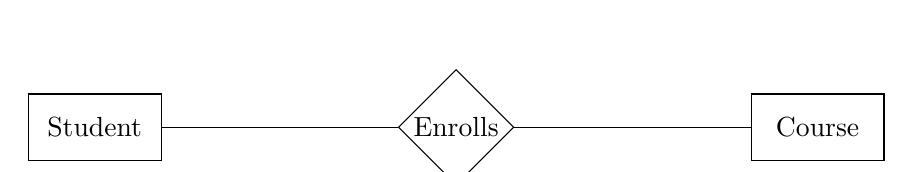
\begin{tikzpicture}[node distance=4cm]
\node[entity] (student) {Student};
\node[relationship, right=3cm of student] (enrolls) {Enrolls};
\node[entity, right=3cm of enrolls] (course) {Course};

\draw (student) -- (enrolls);
\draw (enrolls) -- (course);
\end{tikzpicture}
\end{center}

\section{Cardinality: The Mathematics of Relationships}

\begin{key}
Cardinality specifies: "How many of Entity A can relate to how many of Entity B?"

This is THE most important concept for database design!
\end{key}

\subsection{The Three Basic Types}

\subsubsection{One-to-One (1:1)}

\begin{intuition}
One entity of type A relates to \textbf{at most one} entity of type B, and vice versa.

Real-world analogy: One person has one passport, one passport belongs to one person.
\end{intuition}

\begin{example}
\textbf{Relationship}: Person $\leftrightarrow$ Passport

\begin{center}
\begin{tabular}{|c|c|}
\hline
\textbf{Person} & \textbf{Passport Number} \\
\hline
Alice & P123456 \\
Bob & P234567 \\
Carol & P345678 \\
\hline
\end{tabular}
\end{center}

Each person has exactly one passport number. Each passport number belongs to exactly one person.

ER Diagram notation:
\begin{center}
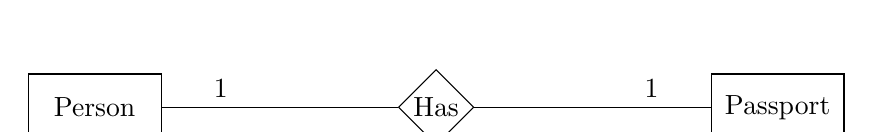
\begin{tikzpicture}[node distance=4cm]
\node[entity] (person) {Person};
\node[relationship, right=3cm of person] (has) {Has};
\node[entity, right=3cm of has] (passport) {Passport};

\draw (person) -- node[above, near start] {1} (has);
\draw (has) -- node[above, near end] {1} (passport);
\end{tikzpicture}
\end{center}
\end{example}

\subsubsection{One-to-Many (1:N)}

\begin{intuition}
One entity of type A can relate to \textbf{many} entities of type B, but each B relates to \textbf{at most one} A.

Real-world analogy: One mother has many children, but each child has one biological mother.
\end{intuition}

\begin{example}
\textbf{Relationship}: Department $\leftrightarrow$ Employee

\begin{center}
\begin{tabular}{|c|c|}
\hline
\textbf{Employee} & \textbf{Department} \\
\hline
Alice & Sales \\
Bob & Sales \\
Carol & Sales \\
David & IT \\
Eve & IT \\
\hline
\end{tabular}
\end{center}

Sales department has 3 employees. Each employee belongs to one department.

ER Diagram notation:
\begin{center}
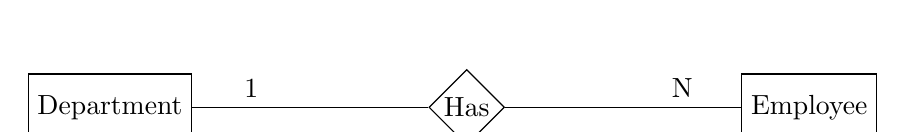
\begin{tikzpicture}[node distance=4cm]
\node[entity] (dept) {Department};
\node[relationship, right=3cm of dept] (has) {Has};
\node[entity, right=3cm of has] (emp) {Employee};

\draw (dept) -- node[above, near start] {1} (has);
\draw (has) -- node[above, near end] {N} (emp);
\end{tikzpicture}
\end{center}

Alternative notation: Crow's foot
\begin{center}
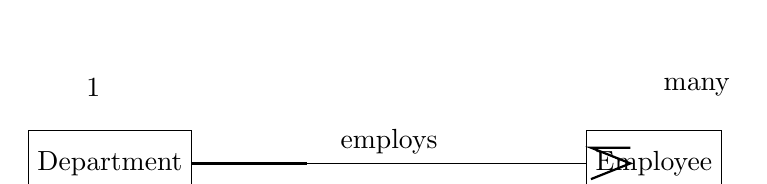
\begin{tikzpicture}[node distance=5cm]
\node[entity] (dept) {Department};
\node[entity, right=5cm of dept] (emp) {Employee};

\draw (dept) -- node[above, midway] {employs} (emp);
\draw[thick] (dept) -- ++(2.5cm, 0);
\draw[thick] (emp) ++(-0.3cm, 0.2cm) -- ++(-0.5cm, 0) -- ++(0.5cm, -0.2cm) -- ++(-0.5cm, -0.2cm);
\node[above=0.3cm of dept, anchor=south east] {1};
\node[above=0.3cm of emp, anchor=south west] {many};
\end{tikzpicture}
\end{center}
\end{example}

\subsubsection{Many-to-Many (M:N)}

\begin{intuition}
One entity of type A can relate to \textbf{many} entities of type B, AND one entity of type B can relate to \textbf{many} entities of type A.

Real-world analogy: Students take many courses, courses have many students.
\end{intuition}

\begin{example}
\textbf{Relationship}: Student $\leftrightarrow$ Course (via Enrolls)

\begin{center}
\begin{tabular}{|c|c|}
\hline
\textbf{Student} & \textbf{Courses Enrolled} \\
\hline
Alice & \{Math, Physics, CS\} \\
Bob & \{Math, Chemistry\} \\
Carol & \{Physics, CS\} \\
\hline
\end{tabular}

\vspace{0.5cm}

\begin{tabular}{|c|c|}
\hline
\textbf{Course} & \textbf{Students Enrolled} \\
\hline
Math & \{Alice, Bob\} \\
Physics & \{Alice, Carol\} \\
CS & \{Alice, Carol\} \\
Chemistry & \{Bob\} \\
\hline
\end{tabular}
\end{center}

Alice takes 3 courses. Math has 2 students. This is many-to-many!

ER Diagram notation:
\begin{center}
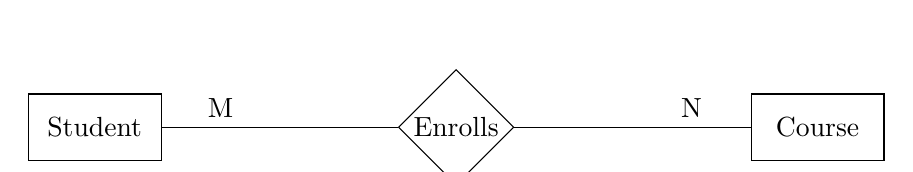
\begin{tikzpicture}[node distance=4cm]
\node[entity] (student) {Student};
\node[relationship, right=3cm of student] (enrolls) {Enrolls};
\node[entity, right=3cm of enrolls] (course) {Course};

\draw (student) -- node[above, near start] {M} (enrolls);
\draw (enrolls) -- node[above, near end] {N} (course);
\end{tikzpicture}
\end{center}
\end{example}

\subsection{Participation Constraints}

\begin{key}
Participation specifies: "Must every entity participate in the relationship?"

\begin{itemize}
    \item \textbf{Total Participation} (double line): Every entity MUST participate
    \item \textbf{Partial Participation} (single line): Entity MAY participate
\end{itemize}
\end{key}

\begin{example}
Consider: Student $\leftrightarrow$ Course

\textbf{Question 1}: Must every student enroll in at least one course?
\begin{itemize}
    \item If YES $\rightarrow$ Total participation (double line from Student)
    \item If NO (students can be registered but not enrolled yet) $\rightarrow$ Partial participation
\end{itemize}

\textbf{Question 2}: Must every course have at least one student?
\begin{itemize}
    \item If YES $\rightarrow$ Total participation (double line from Course)
    \item If NO (courses can exist without students yet) $\rightarrow$ Partial participation
\end{itemize}

Realistic scenario: Partial participation on both sides.

\begin{center}
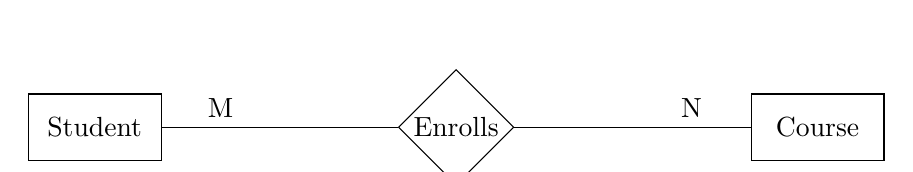
\begin{tikzpicture}[node distance=4cm]
\node[entity] (student) {Student};
\node[relationship, right=3cm of student] (enrolls) {Enrolls};
\node[entity, right=3cm of enrolls] (course) {Course};

% Partial participation - single lines
\draw (student) -- node[above, near start] {M} (enrolls);
\draw (enrolls) -- node[above, near end] {N} (course);
\end{tikzpicture}
\end{center}

With total participation on Student side:
\begin{center}
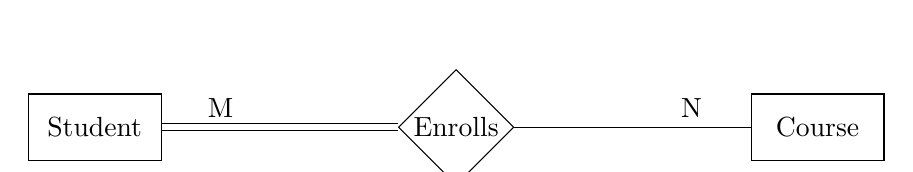
\begin{tikzpicture}[node distance=4cm]
\node[entity] (student) {Student};
\node[relationship, right=3cm of student] (enrolls) {Enrolls};
\node[entity, right=3cm of enrolls] (course) {Course};

% Total participation from Student - double line
\draw[double, double distance=2pt] (student) -- node[above, near start] {M} (enrolls);
\draw (enrolls) -- node[above, near end] {N} (course);
\end{tikzpicture}
\end{center}
\end{example}

\subsection{Calculating Minimum and Maximum Cardinality}

\begin{key}
Modern notation uses (min, max) pairs:

\begin{center}
\textbf{Entity A} —— (min\_A, max\_A) —— Relationship —— (min\_B, max\_B) —— \textbf{Entity B}
\end{center}

\begin{itemize}
    \item min = 0: Partial participation
    \item min $\geq$ 1: Total participation
    \item max = 1: "to-one" relationship
    \item max = N (or *): "to-many" relationship
\end{itemize}
\end{key}

\begin{example}
\textbf{Scenario}: Department-Employee relationship
\begin{itemize}
    \item Each department must have at least 1 employee (can have many)
    \item Each employee must belong to exactly 1 department
\end{itemize}

Analysis:
\begin{itemize}
    \item Department side: min = 1 (must have employees), max = N (can have many)
    \item Employee side: min = 1 (must belong to dept), max = 1 (only one dept)
\end{itemize}

\begin{center}
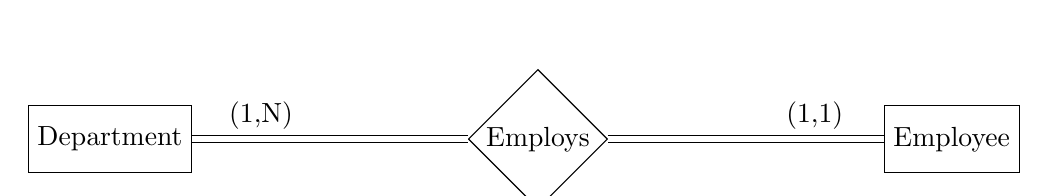
\begin{tikzpicture}[node distance=5cm]
\node[entity] (dept) {Department};
\node[relationship, right=3.5cm of dept] (employs) {Employs};
\node[entity, right=3.5cm of employs] (emp) {Employee};

\draw[double, double distance=2pt] (dept) -- node[above, near start] {(1,N)} (employs);
\draw[double, double distance=2pt] (employs) -- node[above, near end] {(1,1)} (emp);
\end{tikzpicture}
\end{center}

Read as: "Department employs (1 to N) employees. Employee works in (1 to 1) department."
\end{example}

\begin{example}
\textbf{Practice Problem}: University system

Given:
\begin{itemize}
    \item Students can enroll in 0 to 6 courses
    \item Courses must have at least 10 students, maximum 100
\end{itemize}

Solution:
\begin{center}
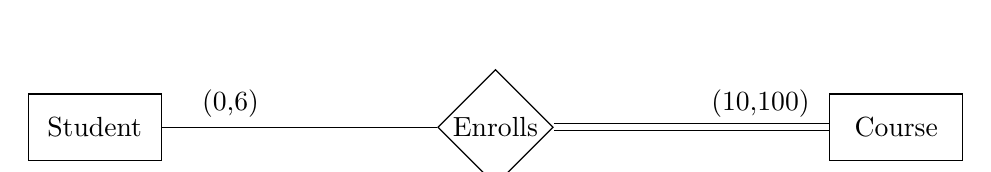
\begin{tikzpicture}[node distance=5cm]
\node[entity] (student) {Student};
\node[relationship, right=3.5cm of student] (enrolls) {Enrolls};
\node[entity, right=3.5cm of enrolls] (course) {Course};

\draw (student) -- node[above, near start] {(0,6)} (enrolls);
\draw[double, double distance=2pt] (enrolls) -- node[above, near end] {(10,100)} (course);
\end{tikzpicture}
\end{center}

Note:
\begin{itemize}
    \item Student has single line (min=0, partial participation)
    \item Course has double line (min=10, total participation)
\end{itemize}
\end{example}

\section{Relationship Attributes}

\begin{intuition}
Sometimes the relationship itself has properties!

Think: When did a student enroll in a course? What grade did they get?

These aren't properties of the student or the course alone—they're properties of the \textit{enrollment relationship}.
\end{intuition}

\begin{example}
Student enrolls in Course:
\begin{itemize}
    \item Enrollment\_Date: When did this enrollment happen?
    \item Grade: What grade did this student get in this course?
    \item Semester: Which semester was this enrollment for?
\end{itemize}

\begin{center}
\begin{tikzpicture}[node distance=3.5cm]
\node[entity] (student) {Student};
\node[relationship, right=3cm of student] (enrolls) {Enrolls};
\node[entity, right=3cm of enrolls] (course) {Course};

% Relationship attributes
\node[attribute, above=1.5cm of enrolls] (date) {Enrollment\_Date} edge (enrolls);
\node[attribute, below=1.5cm of enrolls] (grade) {Grade} edge (enrolls);

\draw (student) -- (enrolls);
\draw (enrolls) -- (course);
\end{tikzpicture}
\end{center}

Data representation:
\begin{center}
\begin{tabular}{|c|c|c|c|}
\hline
\textbf{Student} & \textbf{Course} & \textbf{Enrollment\_Date} & \textbf{Grade} \\
\hline
Alice & Math & 2024-01-15 & A \\
Alice & Physics & 2024-01-16 & B+ \\
Bob & Math & 2024-01-15 & A- \\
Bob & Chemistry & 2024-01-20 & B \\
\hline
\end{tabular}
\end{center}
\end{example}

\begin{warning}
\textbf{Common Mistake}: Putting relationship attributes on an entity

\textbf{Wrong}: Making "Grade" an attribute of Student
\begin{itemize}
    \item Problem: A student has different grades for different courses!
\end{itemize}

\textbf{Wrong}: Making "Grade" an attribute of Course
\begin{itemize}
    \item Problem: Different students get different grades in the same course!
\end{itemize}

\textbf{Correct}: Grade is an attribute of the \textit{Enrolls} relationship
\end{warning}

\section{Weak Entities: Dependent Existence}

\begin{key}
A \textbf{weak entity}:
\begin{enumerate}
    \item Cannot exist without another entity (the \textbf{owner/identifying entity})
    \item Does not have its own unique key
    \item Identified by: (partial key) + (owner's key)
\end{enumerate}
\end{key}

\begin{intuition}
Think of a hotel room. "Room 101" only makes sense if you know \textit{which hotel}. Room 101 at Hilton $\neq$ Room 101 at Marriott.

The room is a weak entity. The hotel is the owner entity.
\end{intuition}

\begin{example}
\textbf{Scenario}: Dependents of employees

\begin{itemize}
    \item Employee: John Smith (ID: E123)
    \item Dependents: Sarah (daughter), Michael (son)
\end{itemize}

Problem: "Sarah" is not unique—many employees might have dependents named Sarah.

Solution: Identify dependents by (Dependent\_Name + Employee\_ID)
\begin{itemize}
    \item (Sarah, E123): John's daughter
    \item (Sarah, E456): Mary's daughter (different person)
\end{itemize}

\begin{center}
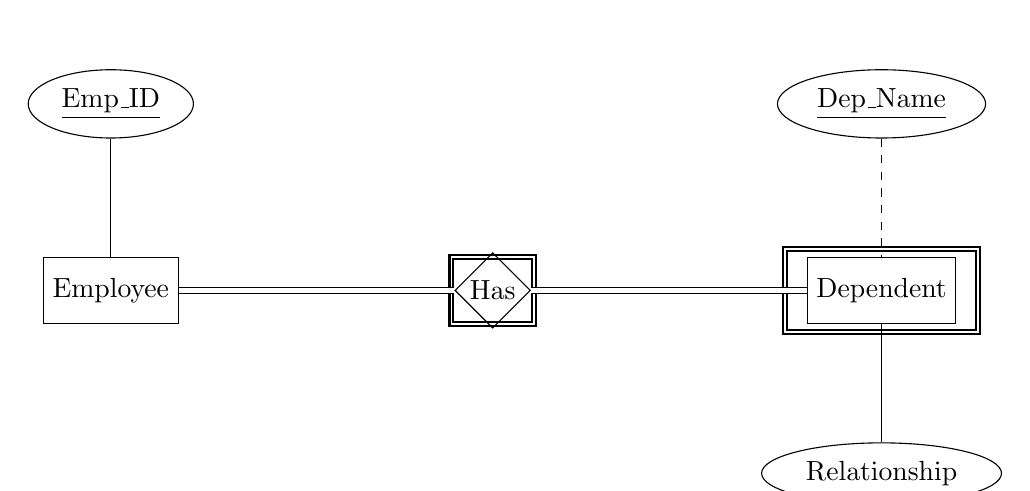
\begin{tikzpicture}[node distance=4cm]
% Owner entity (double rectangle for weak entity's owner shown differently)
\node[entity] (emp) {Employee};

% Identifying relationship (double diamond)
\node[relationship, right=3.5cm of emp] (has) {Has};
\draw[thick] (has) ++(-0.5, -0.4) rectangle ++(1, 0.8);
\draw[thick] (has) ++(-0.55, -0.45) rectangle ++(1.1, 0.9);

% Weak entity (double rectangle)
\node[entity, right=3.5cm of has] (dep) {Dependent};
\draw[thick] (dep) ++(-1.2, -0.5) rectangle ++(2.4, 1);
\draw[thick] (dep) ++(-1.25, -0.55) rectangle ++(2.5, 1.1);

% Partial key (dashed underline)
\node[attribute, above=1.5cm of dep] (name) {\underline{Dep\_Name}} edge[dashed] (dep);
\node[attribute, below=1.5cm of dep] (relation) {Relationship} edge (dep);

% Employee attributes
\node[attribute, above=1.5cm of emp] (eid) {\underline{Emp\_ID}} edge (emp);

% Total participation from weak entity
\draw[double, double distance=2pt] (emp) -- (has);
\draw[double, double distance=2pt] (has) -- (dep);
\end{tikzpicture}
\end{center}

Notation:
\begin{itemize}
    \item Weak entity: Double rectangle
    \item Identifying relationship: Double diamond
    \item Partial key: Dashed underline
    \item Always total participation from weak entity
\end{itemize}
\end{example}

\begin{example}
\textbf{Practice}: University sections

\begin{itemize}
    \item Course: "Database Systems" (CS601)
    \item Sections: Section 1 (Monday 9AM), Section 2 (Wednesday 2PM)
\end{itemize}

Analysis:
\begin{itemize}
    \item "Section 1" meaningless without knowing which course
    \item Section is weak entity, Course is owner
    \item Identify section by: (Section\_Number, Course\_ID)
\end{itemize}

\begin{center}
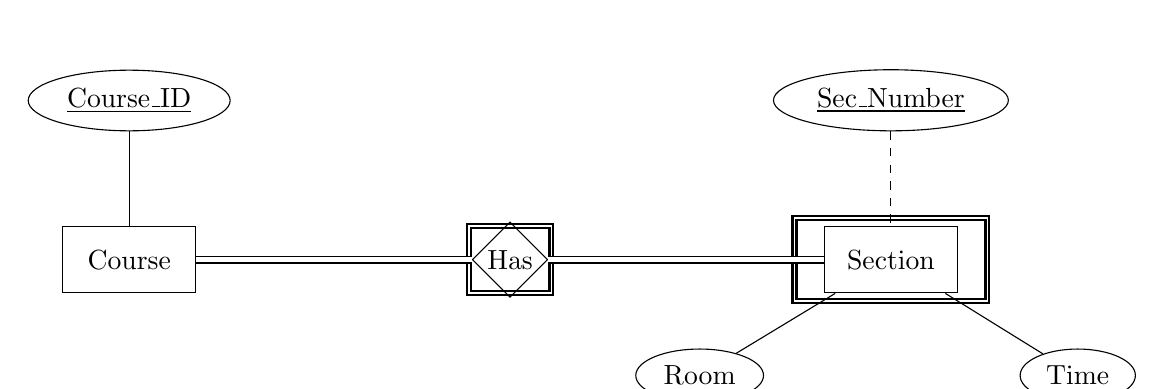
\begin{tikzpicture}[node distance=4cm]
\node[entity] (course) {Course};
\node[relationship, right=3.5cm of course] (has) {Has};
\draw[thick] (has) ++(-0.5, -0.4) rectangle ++(1, 0.8);
\draw[thick] (has) ++(-0.55, -0.45) rectangle ++(1.1, 0.9);

\node[entity, right=3.5cm of has] (section) {Section};
\draw[thick] (section) ++(-1.2, -0.5) rectangle ++(2.4, 1);
\draw[thick] (section) ++(-1.25, -0.55) rectangle ++(2.5, 1.1);

\node[attribute, above=1.2cm of section] (secnum) {\underline{Sec\_Number}} edge[dashed] (section);
\node[attribute, below right=0.8cm and 1cm of section] (time) {Time} edge (section);
\node[attribute, below left=0.8cm and 1cm of section] (room) {Room} edge (section);

\node[attribute, above=1.2cm of course] (cid) {\underline{Course\_ID}} edge (course);

\draw[double, double distance=2pt] (course) -- (has);
\draw[double, double distance=2pt] (has) -- (section);
\end{tikzpicture}
\end{center}

Data:
\begin{center}
\begin{tabular}{|c|c|c|c|}
\hline
\textbf{Course\_ID} & \textbf{Sec\_Number} & \textbf{Time} & \textbf{Room} \\
\hline
CS601 & 1 & Mon 9AM & A101 \\
CS601 & 2 & Wed 2PM & B205 \\
CS602 & 1 & Tue 10AM & A101 \\
\hline
\end{tabular}
\end{center}

Key: (Course\_ID, Sec\_Number) together uniquely identify each section.
\end{example}

\section{Advanced Relationship Types}

\subsection{Recursive Relationships (Self-Relationships)}

\begin{intuition}
An entity can have a relationship with itself!

Examples:
\begin{itemize}
    \item Employees supervise other employees
    \item Courses have prerequisite courses
    \item People are married to people
\end{itemize}
\end{intuition}

\begin{example}
\textbf{Scenario}: Employee supervision hierarchy

\begin{center}
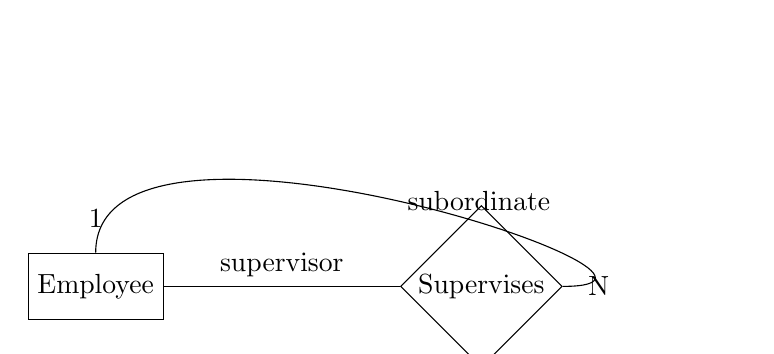
\begin{tikzpicture}[node distance=4cm]
\node[entity] (emp) {Employee};
\node[relationship, right=3cm of emp] (supervises) {Supervises};

% Recursive relationship
\draw (emp) -- node[above] {supervisor} (supervises);
\draw (supervises) to [out=0, in=90] node[right] {subordinate} (emp);

% Add role labels
\node[above=0.2cm of emp] {1};
\node[right=0.2cm of supervises] {N};
\end{tikzpicture}
\end{center}

Data representation:
\begin{center}
\begin{tabular}{|c|c|c|}
\hline
\textbf{Emp\_ID} & \textbf{Name} & \textbf{Supervisor\_ID} \\
\hline
E1 & Alice (CEO) & NULL \\
E2 & Bob & E1 \\
E3 & Carol & E1 \\
E4 & David & E2 \\
E5 & Eve & E2 \\
\hline
\end{tabular}
\end{center}

Interpretation:
\begin{itemize}
    \item Alice supervises Bob and Carol (1:N from supervisor perspective)
    \item Bob is supervised by Alice (N:1 from subordinate perspective)
    \item Alice has no supervisor (CEO)
\end{itemize}

\textbf{Role names} are crucial here to distinguish: supervisor vs. subordinate roles.
\end{example}

\subsection{Ternary Relationships (3-Way)}

\begin{intuition}
Sometimes a relationship involves THREE entities simultaneously.

Can't be broken into binary relationships without losing information!
\end{intuition}

\begin{example}
\textbf{Scenario}: Project assignment in a company

\begin{center}
Question: Who works on which project using what equipment?
\end{center}

Three entities: Employee, Project, Equipment

\begin{center}
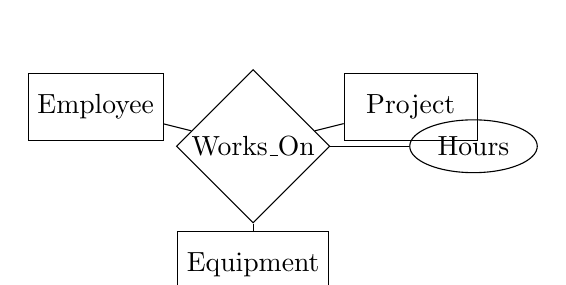
\begin{tikzpicture}[node distance=3.5cm]
\node[entity] (emp) at (0, 2) {Employee};
\node[entity] (proj) at (4, 2) {Project};
\node[entity] (equip) at (2, 0) {Equipment};

\node[relationship] (works) at (2, 1.5) {Works\_On};

\draw (emp) -- (works);
\draw (proj) -- (works);
\draw (equip) -- (works);

% Relationship attribute
\node[attribute, right=1cm of works] (hours) {Hours} edge (works);
\end{tikzpicture}
\end{center}

Example data:
\begin{center}
\begin{tabular}{|c|c|c|c|}
\hline
\textbf{Employee} & \textbf{Project} & \textbf{Equipment} & \textbf{Hours} \\
\hline
Alice & ProjectX & Laptop1 & 40 \\
Alice & ProjectX & Microscope & 20 \\
Bob & ProjectY & Laptop2 & 35 \\
Bob & ProjectZ & Laptop2 & 15 \\
\hline
\end{tabular}
\end{center}

Why ternary? 
\begin{itemize}
    \item Can't split into: (Employee-Project) + (Employee-Equipment)
    \item Because: Alice works on ProjectX with \textit{two different} equipment
    \item The combination of all three matters!
\end{itemize}
\end{example}

\begin{warning}
\textbf{When NOT to use ternary}:

If relationships are independent:
\begin{itemize}
    \item Students enroll in Courses
    \item Students use Library resources
\end{itemize}

These are TWO separate binary relationships, not one ternary!
\end{warning}

\subsection{Aggregation: Relationships on Relationships}

\begin{intuition}
What if you need a relationship that involves another relationship?

Example: Employees are assigned to (Employee works\_on Project) assignments, and managers evaluate these assignments.
\end{intuition}

\begin{example}
\textbf{Scenario}: Project evaluation

\begin{itemize}
    \item Employees work on Projects (relationship 1)
    \item Managers evaluate these work assignments (relationship 2)
\end{itemize}

Can't model with ternary because Manager doesn't directly relate to Employee and Project—they evaluate the \textit{assignment} itself.

Solution: \textbf{Aggregation} - treat (Employee works\_on Project) as a higher-level entity.

\begin{center}
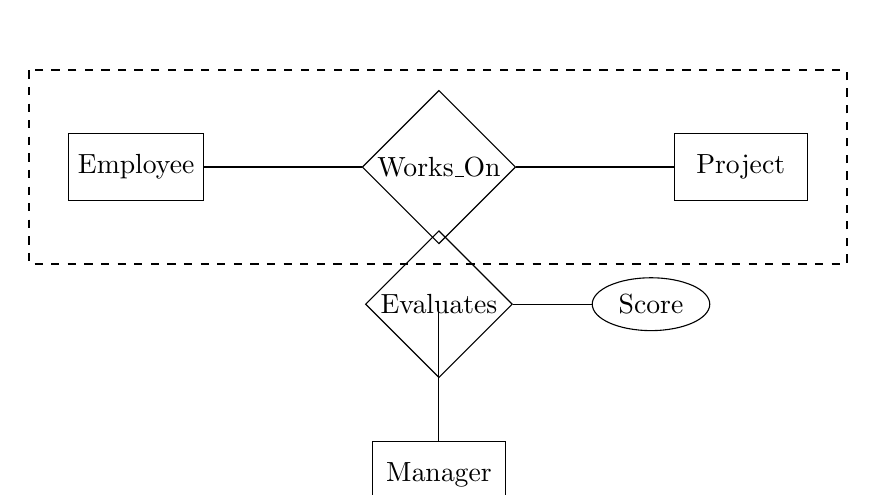
\begin{tikzpicture}[node distance=3cm]
% Inner relationship
\node[entity] (emp) {Employee};
\node[relationship, right=2cm of emp] (works) {Works\_On};
\node[entity, right=2cm of works] (proj) {Project};

\draw (emp) -- (works);
\draw (works) -- (proj);

% Aggregation box
\draw[thick, dashed] ([shift={(-0.5,0.8)}]emp.north west) rectangle ([shift={(0.5,-0.8)}]proj.south east);

% Outer relationship
\node[entity, below=2.5cm of works] (mgr) {Manager};
\node[relationship, above=0.8cm of mgr] (evaluates) {Evaluates};

\draw (evaluates) -- (mgr);
\draw (evaluates) -- ([shift={(0,-0.8)}]works.south);

% Attribute of evaluation
\node[attribute, right=1cm of evaluates] (score) {Score} edge (evaluates);
\end{tikzpicture}
\end{center}

The dashed box represents aggregation: treating the entire "Employee works on Project" as a single entity for the purpose of the Evaluates relationship.
\end{example}

\section{Complete ER Design Example}

\begin{example}
\textbf{Problem}: Design an ER model for a university with these requirements:

\begin{enumerate}
    \item Students have ID, name, email, and phone numbers (multiple possible)
    \item Courses have course code, title, and credits
    \item Professors have ID, name, department, and office
    \item Students enroll in courses with a grade and semester
    \item Professors teach courses in specific semesters
    \item Each course section has a section number, room, and time
    \item Each student has exactly one advisor (who is a professor)
    \item Each department must have at least one professor
\end{enumerate}

\textbf{Step 1}: Identify entities
\begin{itemize}
    \item Student, Course, Professor, Department, Section
\end{itemize}

\textbf{Step 2}: Identify attributes

\begin{tabular}{|l|l|}
\hline
\textbf{Entity} & \textbf{Attributes} \\
\hline
Student & \underline{Student\_ID}, Name, Email, \{Phone\} (multi-valued) \\
Course & \underline{Course\_Code}, Title, Credits \\
Professor & \underline{Prof\_ID}, Name, Office \\
Department & \underline{Dept\_Name}, Building, Office\_Room \\
Section & \underline{Sec\_Number} (partial), Room, Time \\
\hline
\end{tabular}
\pagebreak
\newline
\textbf{Step 3}: Identify relationships

\begin{enumerate}
    \item \textbf{Enrolls}: Student (M) $\leftrightarrow$ (N) Course
    \begin{itemize}
        \item Attributes: Grade, Semester
        \item Cardinality: M:N (students take many courses, courses have many students)
    \end{itemize}
    
    \item \textbf{Teaches}: Professor (M) $\leftrightarrow$ (N) Course
    \begin{itemize}
        \item Attributes: Semester, Year
        \item Cardinality: M:N (professor teaches multiple courses, course taught by multiple professors over time)
    \end{itemize}
    
    \item \textbf{Advises}: Professor (1) $\leftrightarrow$ (N) Student
    \begin{itemize}
        \item Each student has exactly 1 advisor
        \item Each professor can advise multiple students
        \item Cardinality: 1:N
    \end{itemize}
    
    \item \textbf{Belongs\_To}: Professor (N) $\leftrightarrow$ (1) Department
    \begin{itemize}
        \item Each professor belongs to one department
        \item Each department has multiple professors (at least 1)
        \item Cardinality: N:1 with total participation from both sides
    \end{itemize}
    
    \item \textbf{Has\_Section}: Course (1) $\leftrightarrow$ (N) Section
    \begin{itemize}
        \item Section is weak entity (depends on Course)
        \item Identifying relationship
    \end{itemize}
\end{enumerate}

\pagebreak
\textbf{Step 4}: Determine participation constraints

\begin{itemize}
    \item Student in Enrolls: Partial (can be registered but not enrolled yet)
    \item Course in Enrolls: Partial (course can exist before students enroll)
    \item Professor in Teaches: Partial (professor might not teach in current semester)
    \item Professor in Belongs\_To: Total (every professor must belong to a department)
    \item Department in Belongs\_To: Total (requirement: must have at least one professor)
    \item Student in Advises: Total (every student must have an advisor)
    \item Section in Has\_Section: Total (section cannot exist without a course)
\end{itemize}
\textbf{Step 5}: Complete ER Diagram

\begin{center}
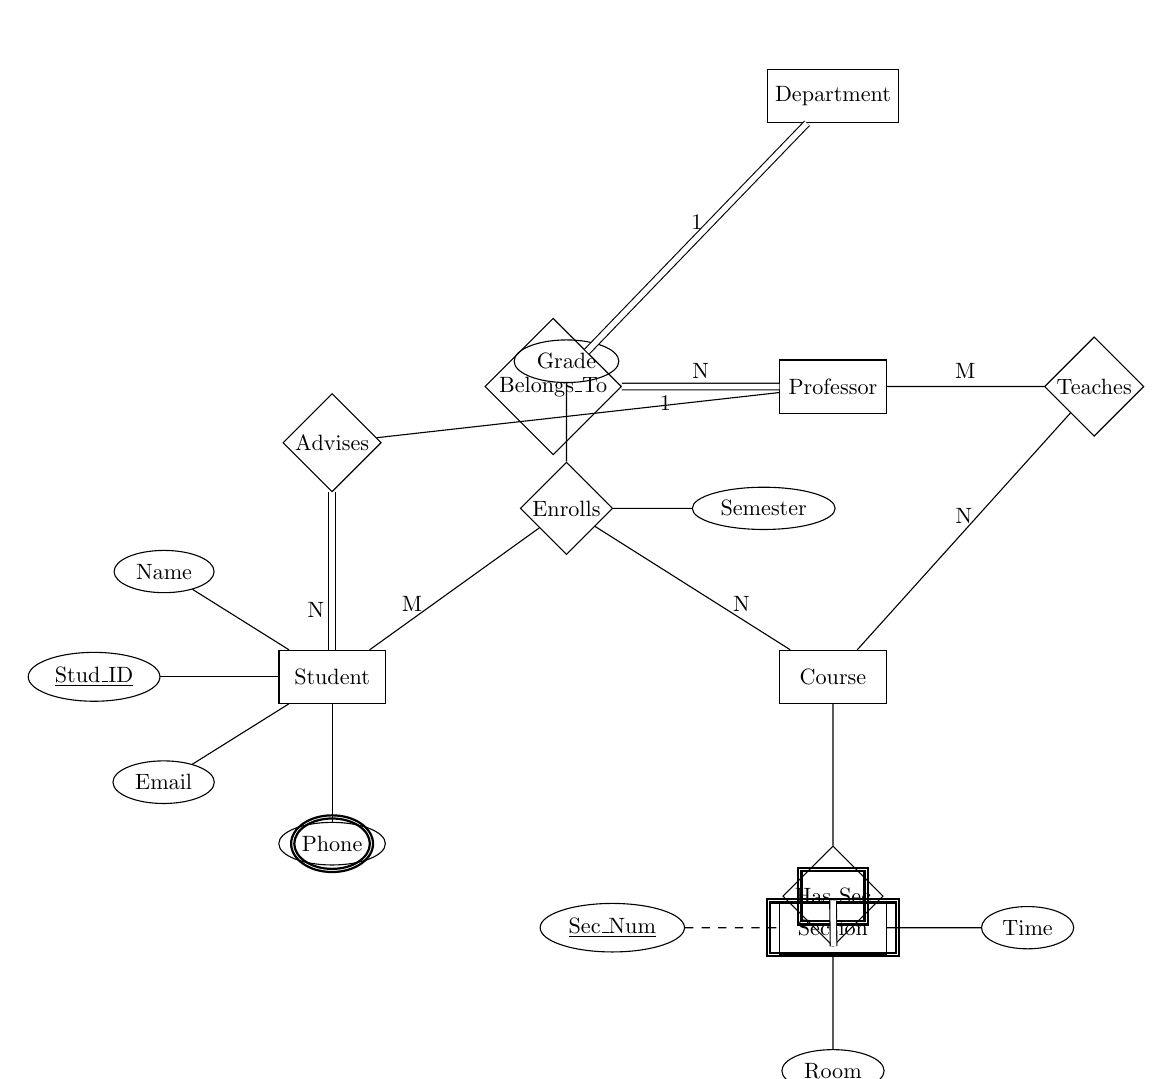
\begin{tikzpicture}[node distance=3cm, scale=0.8, every node/.style={scale=0.8}]
% Entities
\node[entity] (student) {Student};
\node[entity, right=5cm of student] (course) {Course};
\node[entity, above=3cm of course] (prof) {Professor};
\node[entity, above=3cm of prof] (dept) {Department};
\node[entity, below=2.5cm of course] (section) {Section};
\draw[thick] (section) ++(-1.0, -0.4) rectangle ++(2.0, 0.8);
\draw[thick] (section) ++(-1.05, -0.45) rectangle ++(2.1, 0.9);

% Attributes for Student
\node[attribute, left=1.5cm of student] (sid) {\underline{Stud\_ID}} edge (student);
\node[attribute, above left=0.8cm and 1cm of student] (sname) {Name} edge (student);
\node[attribute, below left=0.8cm and 1cm of student] (email) {Email} edge (student);
\node[attribute, below=1.5cm of student] (phone) {Phone} edge (student);
\draw[thick] (phone) ellipse (0.6cm and 0.4cm);
\draw[thick] (phone) ellipse (0.65cm and 0.45cm);

% Enrolls relationship
\node[relationship, above right=1.5cm and 2cm of student] (enrolls) {Enrolls};
\node[attribute, above=1cm of enrolls] (grade) {Grade} edge (enrolls);
\node[attribute, right=1cm of enrolls] (sem) {Semester} edge (enrolls);

\draw (student) -- node[above, near start] {M} (enrolls);
\draw (enrolls) -- node[above, near end] {N} (course);

% Advises relationship
\node[relationship, above=2cm of student] (advises) {Advises};
\draw (prof) -- node[left, near start] {1} (advises);
\draw[double, double distance=2pt] (advises) -- node[left, near end] {N} (student);

% Teaches relationship
\node[relationship, right=2cm of prof] (teaches) {Teaches};
\draw (prof) -- node[above] {M} (teaches);
\draw (teaches) -- node[above] {N} (course);

% Belongs_To relationship
\node[relationship, left=2cm of prof] (belongs) {Belongs\_To};
\draw[double, double distance=2pt] (prof) -- node[above] {N} (belongs);
\draw[double, double distance=2pt] (belongs) -- node[above] {1} (dept);

% Has_Section (identifying relationship)
\node[relationship, below=1.8cm of course] (hassec) {Has\_Sec};
\draw[thick] (hassec) ++(-0.5, -0.4) rectangle ++(1, 0.8);
\draw[thick] (hassec) ++(-0.55, -0.45) rectangle ++(1.1, 0.9);

\draw (course) -- (hassec);
\draw[double, double distance=2pt] (hassec) -- (section);

% Section partial key
\node[attribute, left=1.2cm of section] (secnum) {\underline{Sec\_Num}} edge[dashed] (section);
\node[attribute, below=1.2cm of section] (room) {Room} edge (section);
\node[attribute, right=1.2cm of section] (time) {Time} edge (section);

\end{tikzpicture}
\end{center}
\end{example}


\section{From ER Model to Tables: A Preview}

\begin{intuition}
The ER model is our blueprint. Eventually, we'll convert it to tables (relations). Here's a quick preview:

\textbf{Entity} $\rightarrow$ Table with entity's attributes as columns

\textbf{Relationship}:
\begin{itemize}
    \item 1:1 - Merge into one table or add foreign key
    \item 1:N - Add foreign key to the "N" side table
    \item M:N - Create a new junction table
\end{itemize}

We'll cover this in detail in the next chapter on the Relational Model.
\end{intuition}

\section{Common Design Patterns and Pitfalls}

\subsection{Design Pattern 1: Reification}

\begin{key}
\textbf{Reification}: Converting an attribute or relationship into an entity when you need to store more information about it.
\end{key}

\begin{example}
\textbf{Initial design}: Student has attribute "Major"

\textbf{Problem}: What if you need to know:
\begin{itemize}
    \item Required credits for the major?
    \item Department offering the major?
    \item When the student declared this major?
\end{itemize}

\textbf{Solution}: Make "Major" an entity!

\begin{center}
Student —— (M:N) —— Declares —— Major
\end{center}

Declares relationship has attributes: Date\_Declared, Status (Primary/Secondary)
\end{example}

\subsection{Design Pattern 2: Inheritance (ISA Hierarchy)}

\begin{key}
Use ISA (is-a) hierarchy when entities have common attributes but also specialized attributes.
\end{key}

\begin{example}
\textbf{Scenario}: University persons

\begin{itemize}
    \item All persons have: ID, Name, DOB, Address
    \item Students additionally have: GPA, Year, Major
    \item Professors additionally have: Rank, Salary, Office
    \item Staff additionally have: Position, Department
\end{itemize}

\textbf{Solution}: ISA hierarchy

\begin{center}
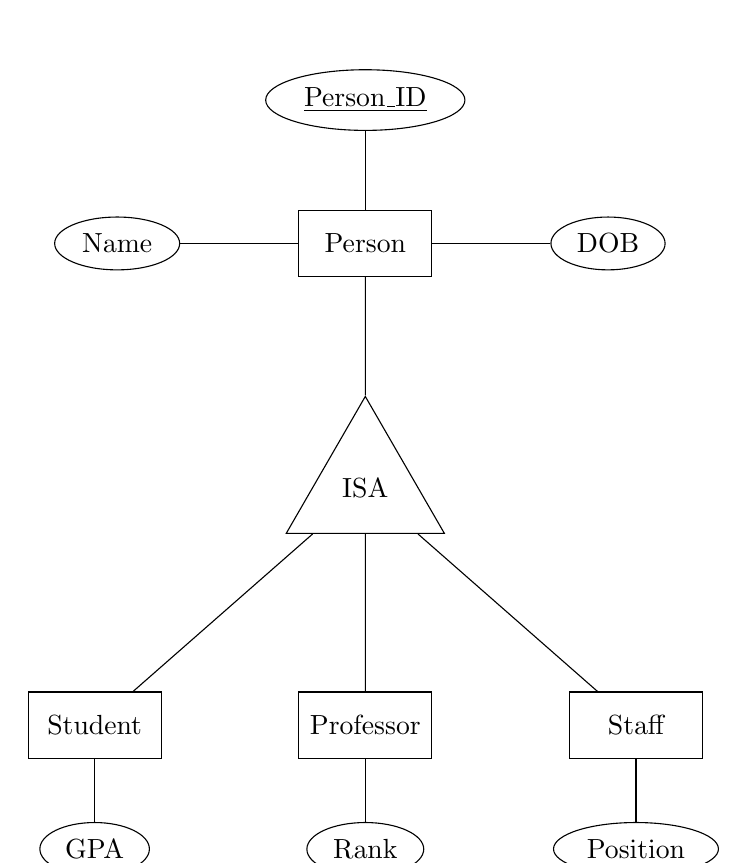
\begin{tikzpicture}[node distance=2.5cm]
% Superclass
\node[entity] (person) {Person};
\node[attribute, above=1cm of person] (pid) {\underline{Person\_ID}} edge (person);
\node[attribute, left=1.5cm of person] (name) {Name} edge (person);
\node[attribute, right=1.5cm of person] (dob) {DOB} edge (person);

% ISA triangle
\node[draw, regular polygon, regular polygon sides=3, below=1.5cm of person, minimum size=1cm] (isa) {ISA};
\draw (person) -- (isa);

% Subclasses
\node[entity, below left=2cm and 2cm of isa] (student) {Student};
\node[entity, below=2cm of isa] (prof) {Professor};
\node[entity, below right=2cm and 2cm of isa] (staff) {Staff};

\draw (isa) -- (student);
\draw (isa) -- (prof);
\draw (isa) -- (staff);

% Specialized attributes
\node[attribute, below=0.8cm of student] (gpa) {GPA} edge (student);
\node[attribute, below=0.8cm of prof] (rank) {Rank} edge (prof);
\node[attribute, below=0.8cm of staff] (pos) {Position} edge (staff);
\end{tikzpicture}
\end{center}

\textbf{Constraint options}:
\begin{enumerate}
    \item \textbf{Overlapping} vs. \textbf{Disjoint}: Can someone be both Student and Professor? (Teaching Assistant)
    \item \textbf{Total} vs. \textbf{Partial}: Must every Person be one of these subtypes?
\end{enumerate}
\end{example}

\subsection{Common Pitfall 1: Redundant Relationships}

\begin{warning}
\textbf{Problem}: Creating relationships that can be derived from existing relationships

\textbf{Example}:
\begin{itemize}
    \item Student enrolls in Course
    \item Course belongs to Department
    \item Student belongs to Department (redundant!)
\end{itemize}

The student's department can be derived from their courses. Don't create the third relationship!

\textbf{Exception}: If you need to store when the relationship was established or need different semantics (student's home department vs. course department).
\end{warning}

\subsection{Common Pitfall 2: Missing Entities}

\begin{warning}
\textbf{Problem}: Treating entities as attributes

\textbf{Wrong}:
\begin{center}
Student has attribute "Advisor\_Name"
\end{center}

\textbf{Right}:
\begin{center}
Student —— (N:1) —— Advised\_By —— Professor
\end{center}

\textbf{Why?} Because Professor is a real entity with its own attributes (ID, office, department, etc.). Don't reduce it to just a name!
\end{warning}

\subsection{Common Pitfall 3: Wrong Cardinality}

\begin{warning}
Carefully analyze real-world constraints!

\textbf{Example}: Customer-Order

\textbf{Wrong assumption}: One customer, one order (1:1)

\textbf{Reality}: One customer, many orders (1:N)

\textbf{To determine cardinality}, ask:
\begin{enumerate}
    \item Can one A relate to multiple B's? (A:many relationship)
    \item Can one B relate to multiple A's? (many:B relationship)
\end{enumerate}

Both yes $\rightarrow$ M:N\\
First yes, second no $\rightarrow$ 1:N\\
Both no $\rightarrow$ 1:1
\end{warning}

\section{Practice Problems with Solutions}

\subsection{Problem 1: Library System}

\textbf{Requirements}:
\begin{itemize}
    \item Track books, members, and loans
    \item Books have ISBN (unique), title, author, publisher
    \item Members have member\_ID, name, address, phone
    \item A book can have multiple copies (same ISBN, different copy numbers)
    \item Members can borrow multiple copies
    \item Track loan date, due date, return date for each loan
\end{itemize}

\textbf{Solution}:

\textbf{Entities}:
\begin{enumerate}
    \item Book: \underline{ISBN}, Title, Author, Publisher
    \item Copy: \underline{Copy\_Number} (partial key), Purchase\_Date, Condition
    \item Member: \underline{Member\_ID}, Name, Address, Phone
\end{enumerate}

\textbf{Relationships}:
\begin{enumerate}
    \item Has\_Copy: Book (1) $\leftrightarrow$ (N) Copy 
    [identifying relationship, Copy is weak]
    
    \item Borrows: Member (M) $\leftrightarrow$ (N) Copy
    \begin{itemize}
        \item Attributes: Loan\_Date, Due\_Date, Return\_Date
    \end{itemize}
\end{enumerate}

\textbf{Key insight}: Copy is a weak entity because ``Copy~1'' only makes sense in the context of a specific book.

\textbf{Why not Member $\leftrightarrow$ Book?} Because we need to track 
\textit{which specific copy} was borrowed!

\subsection{Problem 2: Hospital Management}

\textbf{Requirements}:
\begin{itemize}
    \item Track patients, doctors, appointments, and prescriptions
    \item Patients have patient\_ID, name, DOB, address
    \item Doctors have doctor\_ID, name, specialization, room\_number
    \item Appointments have appointment\_ID, date, time, reason
    \item Prescriptions include medicine name, dosage, duration
    \item Each appointment is between one patient and one doctor
    \item One appointment can have multiple prescriptions
\end{itemize}

\textbf{Solution}:

\textbf{Entities}:
\begin{enumerate}
    \item Patient: \underline{Patient\_ID}, Name, DOB, Address
    \item Doctor: \underline{Doctor\_ID}, Name, Specialization, Room\_Number
    \item Appointment: \underline{Appointment\_ID}, Date, Time, Reason
    \item Medicine: \underline{Medicine\_Name}, Manufacturer, Price
\end{enumerate}

\textbf{Relationships}:
\begin{enumerate}
    \item Has\_Appointment: Patient (1) $\leftrightarrow$ (N) Appointment
    \item Conducts: Doctor (1) $\leftrightarrow$ (N) Appointment
    \item Prescribes: Appointment (M) $\leftrightarrow$ (N) Medicine
    \begin{itemize}
        \item Attributes: Dosage, Duration, Instructions
    \end{itemize}
\end{enumerate}

\textbf{Design decision}: Appointment is an entity (not just a relationship) because:
\begin{itemize}
    \item It has its own unique ID
    \item It has multiple attributes (date, time, reason)
    \item Other entities (Prescription) relate to it
\end{itemize}

\subsection{Problem 3: Course Prerequisites}

\textbf{Requirements}:
\begin{itemize}
    \item Some courses require other courses as prerequisites
    \item A course can have multiple prerequisites
    \item A course can be a prerequisite for multiple courses
\end{itemize}

\textbf{Solution}:

This is a \textbf{recursive M:N relationship}!

\begin{center}
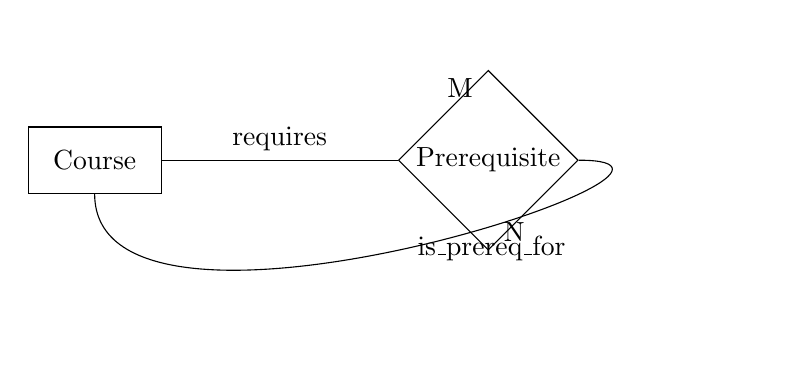
\begin{tikzpicture}[node distance=3.5cm]
\node[entity] (course) {Course};
\node[relationship, right=3cm of course] (prereq) {Prerequisite};

\draw (course) -- node[above] {requires} (prereq);
\draw (prereq) to [out=0, in=-90] node[right] {is\_prereq\_for} (course);

\node[above left=0.1cm and -0.5cm of prereq] {M};
\node[below right=0.1cm and -0.5cm of prereq] {N};
\end{tikzpicture}
\end{center}
\pagebreak
\textbf{Example data}:
\begin{center}
\begin{tabular}{|c|c|}
\hline
\textbf{Course} & \textbf{Prerequisites} \\
\hline
Data Structures & Programming-I \\
Algorithms & Data Structures, Discrete Math \\
Database Systems & Data Structures \\
Operating Systems & Data Structures, Computer Arch \\
\hline
\end{tabular}
\end{center}

\section{Summary and Key Takeaways}

\begin{key}
\textbf{ER Model Checklist}:

\begin{enumerate}
    \item \textbf{Identify Entities}: Nouns that need data stored
    \item \textbf{Identify Attributes}: Properties of each entity
    \begin{itemize}
        \item Mark key attributes
        \item Identify composite, multi-valued, derived attributes
    \end{itemize}
    \item \textbf{Identify Relationships}: How entities connect
    \begin{itemize}
        \item Determine cardinality (1:1, 1:N, M:N)
        \item Determine participation (total/partial)
        \item Add relationship attributes if needed
    \end{itemize}
    \item \textbf{Identify Weak Entities}: Entities dependent on others
    \item \textbf{Consider Special Cases}:
    \begin{itemize}
        \item Recursive relationships
        \item Ternary relationships
        \item ISA hierarchies
    \end{itemize}
\end{enumerate}
\end{key}
\pagebreak
\begin{key}
\textbf{Notation Summary}:

\begin{center}
\begin{tabular}{|l|l|}
\hline
\textbf{Concept} & \textbf{Notation} \\
\hline
Entity & Rectangle \\
Weak Entity & Double Rectangle \\
Attribute & Ellipse \\
Key Attribute & Underlined \\
Partial Key & Dashed Underline \\
Multi-valued Attribute & Double Ellipse \\
Derived Attribute & Dashed Ellipse \\
Relationship & Diamond \\
Identifying Relationship & Double Diamond \\
Total Participation & Double Line \\
Partial Participation & Single Line \\
Cardinality & Numbers (1, N, M) or (min, max) \\
ISA Hierarchy & Triangle \\
\hline
\end{tabular}
\end{center}
\end{key}

\begin{intuition}
\textbf{Mental Model for ER Design}:

Think of designing a database like organizing a filing cabinet:
\begin{enumerate}
    \item \textbf{Entities} = Types of folders (Student files, Course files)
    \item \textbf{Attributes} = Information on each document in a folder
    \item \textbf{Relationships} = Cross-references between folders
    \item \textbf{Keys} = Unique labels on each folder
    \item \textbf{Cardinality} = How many cross-references are allowed
\end{enumerate}

The goal: Design it so anyone can find any information quickly and correctly!
\end{intuition}

\section{Exercises for Practice}

\subsection{Exercise 1: E-Commerce System}

Design an ER model for an online shopping system with:
\begin{itemize}
    \item Customers place orders
    \item Orders contain multiple products
    \item Products belong to categories
    \item Each order has a shipping address
    \item Track order status (pending, shipped, delivered)
    \item Customers can review products (rating and comment)
\end{itemize}

\textbf{Hint}: Think about what should be entities vs. attributes. Should "shipping address" be an attribute or entity? Should "order status" be an attribute or entity?

\subsection{Exercise 2: Social Media Platform}

Design an ER model for a social media platform where:
\begin{itemize}
    \item Users create posts (text, images, or videos)
    \item Users can follow other users
    \item Users can like and comment on posts
    \item Posts can have hashtags
    \item Users can send direct messages to each other
\end{itemize}

\textbf{Hint}: Multiple recursive relationships! User follows User, User messages User.

\subsection{Exercise 3: School Timetable}

Design an ER model for a school timetable system with:
\begin{itemize}
    \item Classes are scheduled in specific rooms at specific times
    \item Teachers teach multiple classes
    \item Students attend multiple classes
    \item Some classes require specific equipment (lab equipment, projectors)
    \item Classes are part of different subjects (Math, Science, etc.)
    \item Track attendance for each class session
\end{itemize}

\textbf{Hint}: Think about ternary relationships. Is there a relationship between Teacher-Class-Room-Time?

\vspace{1cm}

\textit{In the next chapter, we'll learn how to convert these ER diagrams into actual database tables using the Relational Model!}

\pagebreak
\newpage
\section*{Chapter 2: Relational Model and Relational Algebra}
\addcontentsline{toc}{section}{Chapter 2: Relational Model and Relational Algebra}

\section{From ER Model to Relational Model}

\begin{intuition}
In Chapter 1, we created blueprints (ER diagrams). Now we build the actual house (database tables).

Think of it like this:
\begin{itemize}
    \item \textbf{ER Model}: Conceptual design (how humans think)
    \item \textbf{Relational Model}: Implementation (how computers store)
\end{itemize}

The relational model uses \textbf{tables} (also called \textbf{relations}) - just like Excel spreadsheets, but with strict mathematical rules.
\end{intuition}

\subsection{What is a Relation?}

\begin{key}
A \textbf{relation} is a table with:
\begin{enumerate}
    \item \textbf{Rows} (tuples): Individual records
    \item \textbf{Columns} (attributes): Properties of records
    \item \textbf{Domain}: Set of allowed values for each attribute
\end{enumerate}

Mathematical definition: $R \subseteq D_1 \times D_2 \times \ldots \times D_n$

Where $D_i$ is the domain of the $i^{th}$ attribute.
\end{key}

\begin{example}
\textbf{Student Relation}:

\begin{center}
\begin{tabular}{|c|c|c|c|}
\hline
\textbf{Student\_ID} & \textbf{Name} & \textbf{Age} & \textbf{Major} \\
\hline
S001 & Alice & 20 & CS \\
S002 & Bob & 21 & Math \\
S003 & Carol & 19 & CS \\
S004 & David & 22 & Physics \\
\hline
\end{tabular}
\end{center}

Breaking it down:
\begin{itemize}
    \item \textbf{Relation name}: Student
    \item \textbf{Attributes}: \{Student\_ID, Name, Age, Major\}
    \item \textbf{Degree}: 4 (number of attributes)
    \item \textbf{Cardinality}: 4 (number of tuples/rows)
    \item \textbf{Domains}:
    \begin{itemize}
        \item Student\_ID: Strings starting with 'S'
        \item Name: Strings
        \item Age: Integers [17, 25]
        \item Major: \{CS, Math, Physics, Chemistry\}
    \end{itemize}
\end{itemize}
\end{example}

\subsection{Properties of Relations}

\begin{key}
Relations have these CRITICAL properties:

\begin{enumerate}
    \item \textbf{No duplicate tuples}: Each row must be unique
    \item \textbf{Unordered tuples}: Row order doesn't matter
    \item \textbf{Unordered attributes}: Column order doesn't matter (theoretically)
    \item \textbf{Atomic values}: Each cell contains single, indivisible value
    \item \textbf{Same domain}: All values in a column from same domain
\end{enumerate}
\end{key}

\begin{example}
\textbf{Valid relation}:

\begin{center}
\begin{tabular}{|c|c|}
\hline
\textbf{Student\_ID} & \textbf{Name} \\
\hline
S001 & Alice \\
S002 & Bob \\
\hline
\end{tabular}
\end{center}

\textbf{Invalid relation} (duplicate tuples):

\begin{center}
\begin{tabular}{|c|c|}
\hline
\textbf{Student\_ID} & \textbf{Name} \\
\hline
S001 & Alice \\
S001 & Alice \\  % DUPLICATE!
\hline
\end{tabular}
\end{center}

\textbf{Invalid relation} (non-atomic values):

\begin{center}
\begin{tabular}{|c|c|}
\hline
\textbf{Student\_ID} & \textbf{Phone\_Numbers} \\
\hline
S001 & \{555-1234, 555-5678\} \\  % Multiple values!
\hline
\end{tabular}
\end{center}

To fix: Create separate rows or separate table.
\end{example}

\subsection{Keys in Relational Model}

\begin{key}
Different types of keys:

\begin{enumerate}
    \item \textbf{Superkey}: Any set of attributes that uniquely identifies tuples
    \item \textbf{Candidate Key}: Minimal superkey (can't remove any attribute)
    \item \textbf{Primary Key}: Chosen candidate key (underlined)
    \item \textbf{Alternate Key}: Candidate keys not chosen as primary
    \item \textbf{Foreign Key}: Attribute referencing primary key in another relation
\end{enumerate}
\end{key}

\begin{example}
Given Student(\underline{Student\_ID}, Email, Name, Age):

\textbf{Superkeys} (many possible):
\begin{itemize}
    \item \{Student\_ID\}
    \item \{Email\}
    \item \{Student\_ID, Name\}
    \item \{Student\_ID, Email, Name, Age\}
    \item \{Email, Age\}
\end{itemize}

\textbf{Candidate keys} (minimal):
\begin{itemize}
    \item \{Student\_ID\} - minimal, unique
    \item \{Email\} - minimal, unique
\end{itemize}

\textbf{Primary key}: Student\_ID (we choose this one)

\textbf{Alternate key}: Email

Why not \{Student\_ID, Name\}? Not minimal - we can remove Name and still have uniqueness.
\end{example}

\begin{example}
\textbf{Foreign Key Example}:

\textbf{Student}(\underline{Student\_ID}, Name, Dept\_Name)\\
\textbf{Department}(\underline{Dept\_Name}, Building, Budget)

Here, Dept\_Name in Student is a \textbf{foreign key} referencing Department.

\begin{center}
Student Table:
\begin{tabular}{|c|c|c|}
\hline
\textbf{Student\_ID} & \textbf{Name} & \textbf{Dept\_Name} \\
\hline
S001 & Alice & CS \\
S002 & Bob & Math \\
S003 & Carol & CS \\
\hline
\end{tabular}

\vspace{0.3cm}

Department Table:
\begin{tabular}{|c|c|c|}
\hline
\textbf{Dept\_Name} & \textbf{Building} & \textbf{Budget} \\
\hline
CS & Engineering & 500000 \\
Math & Sciences & 300000 \\
Physics & Sciences & 400000 \\
\hline
\end{tabular}
\end{center}

\textbf{Referential Integrity}: Every Dept\_Name in Student must exist in Department.

Alice's Dept\_Name = "CS" $checkmark$ (exists in Department)\\
Can't have Dept\_Name = "Music" in Student if Music doesn't exist in Department $crossmark$
\end{example}

\section{Converting ER Model to Relational Model}

\begin{key}
\textbf{Conversion Rules}:

\begin{enumerate}
    \item \textbf{Strong Entity} $\rightarrow$ Table with all attributes
    \item \textbf{Weak Entity} $\rightarrow$ Table with partial key + owner's primary key
    \item \textbf{1:1 Relationship} $\rightarrow$ Foreign key in either table (or merge)
    \item \textbf{1:N Relationship} $\rightarrow$ Foreign key in "N" side
    \item \textbf{M:N Relationship} $\rightarrow$ New junction table
    \item \textbf{Multi-valued Attribute} $\rightarrow$ Separate table
    \item \textbf{Composite Attribute} $\rightarrow$ Flatten or keep components
\end{enumerate}
\end{key}

\subsection{Rule 1: Strong Entity to Table}

\begin{example}
\textbf{ER Model}:

Student entity with attributes: \underline{Student\_ID}, Name, DOB, Email

\textbf{Relational Model}:

Student(\underline{Student\_ID}, Name, DOB, Email)

Simple! Each attribute becomes a column.
\end{example}

\subsection{Rule 2: Weak Entity to Table}

\begin{example}
\textbf{ER Model}:

Course(\underline{Course\_ID}, Title) —— Has —— Section(\underline{Sec\_Num}, Room, Time)

Section is weak, depends on Course.

\textbf{Relational Model}:

Course(\underline{Course\_ID}, Title)\\
Section(\underline{Course\_ID, Sec\_Num}, Room, Time)

Note: Section's primary key = \{Course\_ID, Sec\_Num\}
\begin{itemize}
    \item Course\_ID is foreign key referencing Course
    \item Sec\_Num alone isn't unique
    \item Together they uniquely identify each section
\end{itemize}

\begin{center}
\begin{tabular}{|c|c|c|c|}
\hline
\textbf{Course\_ID} & \textbf{Sec\_Num} & \textbf{Room} & \textbf{Time} \\
\hline
CS601 & 1 & A101 & Mon 9AM \\
CS601 & 2 & B205 & Wed 2PM \\
CS602 & 1 & A101 & Tue 10AM \\
\hline
\end{tabular}
\end{center}
\end{example}

\subsection{Rule 3: One-to-One Relationship}

\begin{example}
\textbf{ER Model}:

Person(\underline{Person\_ID}, Name) —(1:1)— Passport(\underline{Passport\_Num}, Issue\_Date)

\textbf{Option 1}: Add foreign key to either side

Person(\underline{Person\_ID}, Name, Passport\_Num*)\\
Passport(\underline{Passport\_Num}, Issue\_Date)

Or:

Person(\underline{Person\_ID}, Name)\\
Passport(\underline{Passport\_Num}, Issue\_Date, Person\_ID*)

\textbf{Option 2}: Merge into one table (if participation is total on both sides)

Person\_Passport(\underline{Person\_ID}, Name, Passport\_Num, Issue\_Date)

\textbf{Which to choose?}
\begin{itemize}
    \item If one side has total participation: Put foreign key on that side
    \item If both partial: Either side works
    \item If both total and closely related: Merge
\end{itemize}
\end{example}

\subsection{Rule 4: One-to-Many Relationship}

\begin{example}
\textbf{ER Model}:

Department(\underline{Dept\_Name}, Building) —(1:N)— Employee(\underline{Emp\_ID}, Name)

One department has many employees.

\textbf{Relational Model}:

Department(\underline{Dept\_Name}, Building)\\
Employee(\underline{Emp\_ID}, Name, Dept\_Name*)

\textbf{Why foreign key on Employee side?}
\begin{itemize}
    \item Each employee belongs to one department
    \item So one foreign key column in Employee suffices
\end{itemize}

\textbf{Wrong approach}: Putting employee IDs in Department
\begin{itemize}
    \item Would need multi-valued attribute (violates 1NF)
    \item Department(Dept\_Name, Building, \{Emp\_IDs\}) $crossmark$
\end{itemize}

\begin{center}
\begin{tabular}{|c|c|c|}
\hline
\textbf{Emp\_ID} & \textbf{Name} & \textbf{Dept\_Name} \\
\hline
E001 & Alice & CS \\
E002 & Bob & CS \\
E003 & Carol & Math \\
\hline
\end{tabular}
\end{center}
\end{example}

\subsection{Rule 5: Many-to-Many Relationship}

\begin{example}
\textbf{ER Model}:

Student(\underline{Student\_ID}, Name) —(M:N)— Enrolls[Grade, Semester] —— Course(\underline{Course\_ID}, Title)

\textbf{Relational Model}:

Student(\underline{Student\_ID}, Name)\\
Course(\underline{Course\_ID}, Title)\\
Enrolls(\underline{Student\_ID*, Course\_ID*}, Grade, Semester)

\textbf{Junction table} Enrolls:
\begin{itemize}
    \item Primary key = \{Student\_ID, Course\_ID\}
    \item Student\_ID is foreign key to Student
    \item Course\_ID is foreign key to Course
    \item Relationship attributes become regular attributes
\end{itemize}

\begin{center}
Student:
\begin{tabular}{|c|c|}
\hline
\textbf{Student\_ID} & \textbf{Name} \\
\hline
S001 & Alice \\
S002 & Bob \\
\hline
\end{tabular}

\vspace{0.3cm}

Course:
\begin{tabular}{|c|c|}
\hline
\textbf{Course\_ID} & \textbf{Title} \\
\hline
CS101 & Intro to CS \\
MATH201 & Calculus \\
\hline
\end{tabular}

\vspace{0.3cm}

Enrolls:
\begin{tabular}{|c|c|c|c|}
\hline
\textbf{Student\_ID} & \textbf{Course\_ID} & \textbf{Grade} & \textbf{Semester} \\
\hline
S001 & CS101 & A & Fall 2024 \\
S001 & MATH201 & B+ & Fall 2024 \\
S002 & CS101 & A- & Fall 2024 \\
\hline
\end{tabular}
\end{center}

This represents:
\begin{itemize}
    \item Alice takes CS101 (grade A) and MATH201 (grade B+)
    \item Bob takes CS101 (grade A-)
\end{itemize}
\end{example}

\subsection{Rule 6: Multi-valued Attributes}

\begin{example}
\textbf{ER Model}:

Student(\underline{Student\_ID}, Name, \{Phone\_Numbers\})

\textbf{Relational Model}:

Student(\underline{Student\_ID}, Name)\\
Student\_Phone(\underline{Student\_ID*, Phone\_Number})

\begin{center}
Student:
\begin{tabular}{|c|c|}
\hline
\textbf{Student\_ID} & \textbf{Name} \\
\hline
S001 & Alice \\
S002 & Bob \\
\hline
\end{tabular}

\vspace{0.3cm}

Student\_Phone:
\begin{tabular}{|c|c|}
\hline
\textbf{Student\_ID} & \textbf{Phone\_Number} \\
\hline
S001 & 555-1234 \\
S001 & 555-5678 \\
S002 & 555-9999 \\
\hline
\end{tabular}
\end{center}

Primary key of Student\_Phone:
\begin{itemize}
    \item Could be \{Student\_ID, Phone\_Number\} (if no duplicates)
    \item Or add a separate Phone\_ID if needed
\end{itemize}
\end{example}

\subsection{Complete Conversion Example}

\begin{example}
\textbf{ER Model}:

\begin{itemize}
    \item Department(\underline{Dept\_Name}, Building, Budget)
    \item Employee(\underline{Emp\_ID}, Name, Salary, \{Skills\})
    \item Project(\underline{Project\_ID}, Title, Budget)
    \item Employee works\_for Department (N:1)
    \item Employee manages Department (1:1, partial)
    \item Employee works\_on Project (M:N) with attribute Hours
\end{itemize}

\textbf{Relational Schema}:

Department(\underline{Dept\_Name}, Building, Budget, Manager\_ID*)\\
Employee(\underline{Emp\_ID}, Name, Salary, Dept\_Name*)\\
Employee\_Skills(\underline{Emp\_ID*, Skill})\\
Project(\underline{Project\_ID}, Title, Budget)\\
Works\_On(\underline{Emp\_ID*, Project\_ID*}, Hours)

Explanation:
\begin{itemize}
    \item Department: Added Manager\_ID (1:1 relationship, FK to Employee)
    \item Employee: Added Dept\_Name (N:1 relationship, FK to Department)
    \item Employee\_Skills: Separate table for multi-valued attribute
    \item Works\_On: Junction table for M:N relationship
\end{itemize}
\end{example}

\section{Relational Algebra: The Mathematical Foundation}

\begin{intuition}
Relational Algebra is the "calculator" for databases. Just like you use +, -, ×, ÷ for numbers, you use relational operators for tables.

Think of it as a way to:
\begin{itemize}
    \item Retrieve data (like asking questions)
    \item Combine tables (like merging spreadsheets)
    \item Filter rows (like using Excel filters)
    \item Select columns (like hiding columns)
\end{itemize}

SQL is based on relational algebra - learning algebra helps you understand SQL deeply!
\end{intuition}

\begin{key}
\textbf{Relational Algebra Operators} (8 fundamental):

\textbf{Basic Operators}:
\begin{enumerate}
    \item \textbf{Select} ($\sigma$): Choose rows
    \item \textbf{Project} ($\pi$): Choose columns
    \item \textbf{Union} ($\cup$): Combine rows from two tables
    \item \textbf{Set Difference} ($-$): Rows in first but not second
    \item \textbf{Cartesian Product} ($\times$): All combinations
    \item \textbf{Rename} ($\rho$): Change attribute/relation names
\end{enumerate}

\textbf{Derived Operators} (combinations of basic):
\begin{enumerate}
    \setcounter{enumi}{6}
    \item \textbf{Intersection} ($\cap$): Common rows
    \item \textbf{Join} ($\bowtie$): Combine based on condition
    \item \textbf{Division} ($\div$): "For all" queries
\end{enumerate}
\end{key}

\subsection{Operator 1: Select ($\sigma$) - Filter Rows}

\begin{key}
\textbf{Select operator}: Chooses rows that satisfy a condition

Notation: $\sigma_{condition}(R)$

Returns: Subset of tuples from R where condition is true
\end{key}

\begin{example}
Given relation Student:

\begin{center}
\begin{tabular}{|c|c|c|c|}
\hline
\textbf{Student\_ID} & \textbf{Name} & \textbf{Age} & \textbf{Major} \\
\hline
S001 & Alice & 20 & CS \\
S002 & Bob & 21 & Math \\
S003 & Carol & 19 & CS \\
S004 & David & 22 & Physics \\
S005 & Eve & 20 & CS \\
\hline
\end{tabular}
\end{center}

\textbf{Query 1}: Find all CS students

$\sigma_{Major = 'CS'}(Student)$

Result:
\begin{center}
\begin{tabular}{|c|c|c|c|}
\hline
\textbf{Student\_ID} & \textbf{Name} & \textbf{Age} & \textbf{Major} \\
\hline
S001 & Alice & 20 & CS \\
S003 & Carol & 19 & CS \\
S005 & Eve & 20 & CS \\
\hline
\end{tabular}
\end{center}

\textbf{Query 2}: Find students aged 20 or more

$\sigma_{Age \geq 20}(Student)$

Result:
\begin{center}
\begin{tabular}{|c|c|c|c|}
\hline
\textbf{Student\_ID} & \textbf{Name} & \textbf{Age} & \textbf{Major} \\
\hline
S001 & Alice & 20 & CS \\
S002 & Bob & 21 & Math \\
S004 & David & 22 & Physics \\
S005 & Eve & 20 & CS \\
\hline
\end{tabular}
\end{center}

\textbf{Query 3}: Find CS students aged 20 or more (compound condition)

$\sigma_{Major = 'CS' \land Age \geq 20}(Student)$

Result:
\begin{center}
\begin{tabular}{|c|c|c|c|}
\hline
\textbf{Student\_ID} & \textbf{Name} & \textbf{Age} & \textbf{Major} \\
\hline
S001 & Alice & 20 & CS \\
S005 & Eve & 20 & CS \\
\hline
\end{tabular}
\end{center}

Conditions can use:
\begin{itemize}
    \item Comparisons: $=, \neq, <, >, \le, \ge$
    \item Logical: $\land$ (AND), $\lor$ (OR), $\neg$ (NOT)
    \item Attributes: Age > 20, Name = 'Alice'
\end{itemize}
\end{example}

\subsection{Operator 2: Project ($\pi$) - Select Columns}

\begin{key}
\textbf{Project operator}: Chooses specific columns (and removes duplicates)

Notation: $\pi_{attribute\_list}(R)$

Returns: Relation with only specified attributes
\end{key}

\begin{example}
Given Student table (same as above):

\textbf{Query 1}: Get only names and majors

$\pi_{Name, Major}(Student)$

Result:
\begin{center}
\begin{tabular}{|c|c|}
\hline
\textbf{Name} & \textbf{Major} \\
\hline
Alice & CS \\
Bob & Math \\
Carol & CS \\
David & Physics \\
Eve & CS \\
\hline
\end{tabular}
\end{center}

\textbf{Query 2}: Get only majors (duplicates removed!)

$\pi_{Major}(Student)$

Result:
\begin{center}
\begin{tabular}{|c|}
\hline
\textbf{Major} \\
\hline
CS \\
Math \\
Physics \\
\hline
\end{tabular}
\end{center}

Note: Even though 3 students are CS majors, "CS" appears only once!

\textbf{Combining Select and Project}:

Get names of CS students:

$\pi_{Name}(\sigma_{Major = 'CS'}(Student))$

Step by step:
\begin{enumerate}
    \item $\sigma_{Major = 'CS'}(Student)$ filters CS students
    \item $\pi_{Name}(...)$ selects only Name column
\end{enumerate}
\pagebreak
Result:
\begin{center}
\begin{tabular}{|c|}
\hline
\textbf{Name} \\
\hline
Alice \\
Carol \\
Eve \\
\hline
\end{tabular}
\end{center}
\end{example}

\subsection{Operator 3: Union ($\cup$) - Combine Tables}

\begin{key}
\textbf{Union operator}: Combines tuples from two relations

Notation: $R \cup S$

\textbf{Requirements}:
\begin{itemize}
    \item R and S must be \textbf{union compatible}:
    \begin{itemize}
        \item Same number of attributes
        \item Corresponding attributes have same domains
    \end{itemize}
\end{itemize}

Returns: All tuples from R and S (duplicates removed)
\end{key}

\begin{example}
CS\_Students:
\begin{center}
\begin{tabular}{|c|c|}
\hline
\textbf{Student\_ID} & \textbf{Name} \\
\hline
S001 & Alice \\
S002 & Bob \\
S003 & Carol \\
\hline
\end{tabular}
\end{center}

Math\_Students:
\begin{center}
\begin{tabular}{|c|c|}
\hline
\textbf{Student\_ID} & \textbf{Name} \\
\hline
S002 & Bob \\
S004 & David \\
S005 & Eve \\
\hline
\end{tabular}
\end{center}

$CS\_Students \cup Math\_Students$:

\begin{center}
\begin{tabular}{|c|c|}
\hline
\textbf{Student\_ID} & \textbf{Name} \\
\hline
S001 & Alice \\
S002 & Bob \\
S003 & Carol \\
S004 & David \\
S005 & Eve \\
\hline
\end{tabular}
\end{center}

Note: Bob (S002) appears in both but listed only once in union!
\end{example}

\subsection{Operator 4: Set Difference ($-$)}

\begin{key}
\textbf{Set Difference operator}: Tuples in first relation but not in second

Notation: $R - S$

Requirements: R and S must be union compatible

Returns: Tuples in R that are not in S
\end{key}

\begin{example}
Using same tables as above:

$CS\_Students - Math\_Students$:

\begin{center}
\begin{tabular}{|c|c|}
\hline
\textbf{Student\_ID} & \textbf{Name} \\
\hline
S001 & Alice \\
S003 & Carol \\
\hline
\end{tabular}
\end{center}

Interpretation: CS students who are NOT math students

$Math\_Students - CS\_Students$:

\begin{center}
\begin{tabular}{|c|c|}
\hline
\textbf{Student\_ID} & \textbf{Name} \\
\hline
S004 & David \\
S005 & Eve \\
\hline
\end{tabular}
\end{center}

Interpretation: Math students who are NOT CS students

Note: Set difference is NOT commutative! $R - S \neq S - R$
\end{example}

\subsection{Operator 5: Cartesian Product ($\times$)}

\begin{key}
\textbf{Cartesian Product}: Combines every tuple from R with every tuple from S

Notation: $R \times S$

Returns: Relation with:
\begin{itemize}
    \item Attributes: All attributes from R and S
    \item Tuples: All possible combinations
    \item Cardinality: $|R| \times |S|$
\end{itemize}
\end{key}

\begin{example}
Student:
\begin{center}
\begin{tabular}{|c|c|}
\hline
\textbf{Student\_ID} & \textbf{Name} \\
\hline
S001 & Alice \\
S002 & Bob \\
\hline
\end{tabular}
\end{center}

Course:
\begin{center}
\begin{tabular}{|c|c|}
\hline
\textbf{Course\_ID} & \textbf{Title} \\
\hline
CS101 & Programming \\
MATH201 & Calculus \\
\hline
\end{tabular}
\end{center}

$Student \times Course$:

\begin{center}
\begin{tabular}{|c|c|c|c|}
\hline
\textbf{Student\_ID} & \textbf{Name} & \textbf{Course\_ID} & \textbf{Title} \\
\hline
S001 & Alice & CS101 & Programming \\
S001 & Alice & MATH201 & Calculus \\
S002 & Bob & CS101 & Programming \\
S002 & Bob & MATH201 & Calculus \\
\hline
\end{tabular}
\end{center}

Result has: 2 × 2 = 4 tuples

\textbf{Warning}: Cartesian product is rarely used alone! Usually filtered immediately.

Example: "All student-course pairs where student is enrolled"

$\sigma_{Student.ID = Enrolled.Stud\_ID \land Enrolled.Course\_ID = Course.ID}(Student \times Enrolled \times Course)$

Better: Use Join (next section)
\end{example}

\subsection{Operator 6: Rename ($\rho$)}

\begin{key}
\textbf{Rename operator}: Changes names of relation or attributes

Notation: 
\begin{itemize}
    \item $\rho_{S}(R)$ - Rename relation R to S
    \item $\rho_{(A_1, A_2, ...)}(R)$ - Rename attributes
    \item $\rho_{S(A_1, A_2, ...)}(R)$ - Rename both
\end{itemize}
\end{key}

\begin{example}
Student:
\begin{center}
\begin{tabular}{|c|c|}
\hline
\textbf{Student\_ID} & \textbf{Name} \\
\hline
S001 & Alice \\
S002 & Bob \\
\hline
\end{tabular}
\end{center}

$\rho_{Pupil}(Student)$ - Relation now called "Pupil"

$\rho_{(ID, Full\_Name)}(Student)$ - Attributes now "ID" and "Full\_Name"

Result:
\begin{center}
\begin{tabular}{|c|c|}
\hline
\textbf{ID} & \textbf{Full\_Name} \\
\hline
S001 & Alice \\
S002 & Bob \\
\hline
\end{tabular}
\end{center}

\textbf{Why rename?} Essential for:
\begin{itemize}
    \item Self-joins (joining table with itself)
    \item Avoiding attribute name conflicts
    \item Making queries more readable
\end{itemize}
\end{example}

\subsection{Operator 7: Intersection ($\cap$) - Derived}

\begin{key}
\textbf{Intersection}: Tuples common to both relations

Notation: $R \cap S$

Derived from: $R \cap S = R - (R - S)$

Or: $R \cap S = (R \cup S) - ((R - S) \cup (S - R))$

Requirements: Union compatible
\end{key}

\begin{example}
CS\_Students:
\begin{center}
\begin{tabular}{|c|c|}
\hline
\textbf{Student\_ID} & \textbf{Name} \\
\hline
S001 & Alice \\
S002 & Bob \\
S003 & Carol \\
\hline
\end{tabular}
\end{center}

Math\_Students:
\begin{center}
\begin{tabular}{|c|c|}
\hline
\textbf{Student\_ID} & \textbf{Name} \\
\hline
S002 & Bob \\
S004 & David \\
\hline
\end{tabular}
\end{center}

$CS\_Students \cap Math\_Students$:

\begin{center}
\begin{tabular}{|c|c|}
\hline
\textbf{Student\_ID} & \textbf{Name} \\
\hline
S002 & Bob \\
\hline
\end{tabular}
\end{center}

Interpretation: Students who are in BOTH CS and Math
\end{example}

\subsection{Operator 8: Join ($\bowtie$) - The Most Important!}

\begin{intuition}
Join is THE most important operation in relational databases!

Think: "Combine tables based on related information"

Like: Matching students with their enrolled courses, employees with their departments, orders with customers.
\end{intuition}

\subsubsection{Theta Join ($\bowtie_\theta$)}

\begin{key}
\textbf{Theta Join}: Cartesian product followed by selection

Notation: $R \bowtie_\theta S$ where $\theta$ is a condition

Equivalent to: $\sigma_\theta(R \times S)$

The condition typically compares attributes from R and S.
\end{key}

\begin{example}
Employee:
\begin{center}
\begin{tabular}{|c|c|c|}
\hline
\textbf{Emp\_ID} & \textbf{Name} & \textbf{Dept\_Name} \\
\hline
E001 & Alice & CS \\
E002 & Bob & Math \\
E003 & Carol & CS \\
\hline
\end{tabular}
\end{center}

Department:
\begin{center}
\begin{tabular}{|c|c|}
\hline
\textbf{Dept\_Name} & \textbf{Building} \\
\hline
CS & Engineering \\
Math & Sciences \\
Physics & Sciences \\
\hline
\end{tabular}
\end{center}

$Employee \bowtie_{Employee.Dept\_Name = Department.Dept\_Name} Department$:

\begin{center}
\small
\setlength{\tabcolsep}{3pt}   % tighter than before
\renewcommand{\arraystretch}{1.05}

\begin{tabular}{|c|c|c|c|c|}
\hline
\textbf{Emp\_ID} & \textbf{Name} & \textbf{Employee.Dept\_Name} & \textbf{Department.Dept\_Name} & \textbf{Building} \\
\hline
E001 & Alice & CS & CS & Engineering \\
E002 & Bob & Math & Math & Sciences \\
E003 & Carol & CS & CS & Engineering \\
\hline
\end{tabular}
\end{center}


Note: Dept\_Name appears twice (from both tables)
\end{example}

\subsubsection{Equi Join}

\begin{key}
\textbf{Equi Join}: Theta join where condition uses only equality (=)

Special case of theta join that's very common!
\end{key}

\subsubsection{Natural Join ($\bowtie$)}

\begin{key}
\textbf{Natural Join}: Equi join on all common attributes, removing duplicates

Notation: $R \bowtie S$

Process:
\begin{enumerate}
    \item Find attributes with same name in R and S
    \item Join on equality of those attributes
    \item Remove duplicate columns
\end{enumerate}
\end{key}

\begin{example}
Same Employee and Department tables:

$Employee \bowtie Department$ (natural join on Dept\_Name):

\begin{center}
\begin{tabular}{|c|c|c|c|}
\hline
\textbf{Emp\_ID} & \textbf{Name} & \textbf{Dept\_Name} & \textbf{Building} \\
\hline
E001 & Alice & CS & Engineering \\
E002 & Bob & Math & Sciences \\
E003 & Carol & CS & Engineering \\
\hline
\end{tabular}
\end{center}

Note: Only ONE Dept\_Name column (duplicates removed)

\textbf{Why Physics department missing?} No employees in Physics!
\end{example}

\subsubsection{Outer Joins - Preserving Unmatched Tuples}

\begin{key}
\textbf{Problem with natural join}: Loses tuples that don't match

\textbf{Solution}: Outer joins preserve unmatched tuples with NULL values

Types:
\begin{enumerate}
    \item \textbf{Left Outer Join} (LEFT JOIN): Keep all tuples from left relation
    \item \textbf{Right Outer Join} (RIGHT JOIN): Keep all tuples from right relation
    \item \textbf{Full Outer Join} (FULL OUTER JOIN): Keep all tuples from both relations
\end{enumerate}

\end{key}

\begin{example}
Employee:
\begin{center}
\begin{tabular}{|c|c|c|}
\hline
\textbf{Emp\_ID} & \textbf{Name} & \textbf{Dept\_Name} \\
\hline
E001 & Alice & CS \\
E002 & Bob & Math \\
E003 & Carol & Biology \\
\hline
\end{tabular}
\end{center}

Department:
\begin{center}
\begin{tabular}{|c|c|}
\hline
\textbf{Dept\_Name} & \textbf{Building} \\
\hline
CS & Engineering \\
Math & Sciences \\
Physics & Sciences \\
\hline
\end{tabular}
\end{center}

Note: Carol works in Biology (not in Department table), Physics has no employees.
\pagebreak
\newline
\textbf{Natural Join} (loses both):
\begin{center}
\begin{tabular}{|c|c|c|c|}
\hline
\textbf{Emp\_ID} & \textbf{Name} & \textbf{Dept\_Name} & \textbf{Building} \\
\hline
E001 & Alice & CS & Engineering \\
E002 & Bob & Math & Sciences \\
\hline
\end{tabular}
\end{center}

\textbf{Left Outer Join} (keeps all employees):
\begin{center}
\begin{tabular}{|c|c|c|c|}
\hline
\textbf{Emp\_ID} & \textbf{Name} & \textbf{Dept\_Name} & \textbf{Building} \\
\hline
E001 & Alice & CS & Engineering \\
E002 & Bob & Math & Sciences \\
E003 & Carol & Biology & NULL \\
\hline
\end{tabular}
\end{center}

\textbf{Right Outer Join} (keeps all departments):
\begin{center}
\begin{tabular}{|c|c|c|c|}
\hline
\textbf{Emp\_ID} & \textbf{Name} & \textbf{Dept\_Name} & \textbf{Building} \\
\hline
E001 & Alice & CS & Engineering \\
E002 & Bob & Math & Sciences \\
NULL & NULL & Physics & Sciences \\
\hline
\end{tabular}
\end{center}

\textbf{Full Outer Join} (keeps both):
\begin{center}
\begin{tabular}{|c|c|c|c|}
\hline
\textbf{Emp\_ID} & \textbf{Name} & \textbf{Dept\_Name} & \textbf{Building} \\
\hline
E001 & Alice & CS & Engineering \\
E002 & Bob & Math & Sciences \\
E003 & Carol & Biology & NULL \\
NULL & NULL & Physics & Sciences \\
\hline
\end{tabular}
\end{center}
\end{example}

\subsection{Operator 9: Division ($\div$) - "For All" Queries}

\begin{key}
\textbf{Division}: Answers "for all" queries

Notation: $R \div S$

Given: $R(X, Y)$ and $S(Y)$

Returns: All X values in R that are associated with ALL Y values in S

Think: "Find X that relates to every Y"
\end{key}

\begin{example}
\textbf{Query}: "Find students enrolled in ALL courses"

Enrolled(Student\_ID, Course\_ID):
\begin{center}
\begin{tabular}{|c|c|}
\hline
\textbf{Student\_ID} & \textbf{Course\_ID} \\
\hline
S001 & CS101 \\
S001 & MATH201 \\
S001 & PHY301 \\
S002 & CS101 \\
S002 & MATH201 \\
S003 & CS101 \\
\hline
\end{tabular}
\end{center}

All\_Courses(Course\_ID):
\begin{center}
\begin{tabular}{|c|}
\hline
\textbf{Course\_ID} \\
\hline
CS101 \\
MATH201 \\
PHY301 \\
\hline
\end{tabular}
\end{center}

$Enrolled \div All\_Courses$:

\begin{center}
\begin{tabular}{|c|}
\hline
\textbf{Student\_ID} \\
\hline
S001 \\
\hline
\end{tabular}
\end{center}

Why?
\begin{itemize}
    \item S001 enrolled in \{CS101, MATH201, PHY301\} - all 3 courses $checkmark$
    \item S002 enrolled in \{CS101, MATH201\} - missing PHY301 $crossmark$
    \item S003 enrolled in \{CS101\} - missing others $crossmark$
\end{itemize}

\textbf{Division Algorithm}:

$R \div S = \pi_X(R) - \pi_X((\pi_X(R) \times S) - R)$

Step by step:
\begin{enumerate}
    \item Get all X values: $\pi_X(R)$ = \{S001, S002, S003\}
    \item Create all possible (X, Y) pairs: $\pi_X(R) \times S$
    \item Find missing pairs: $(\pi_X(R) \times S) - R$
    \item Get X values with missing pairs: $\pi_X(missing)$
    \item Remove them: $\pi_X(R) - \pi_X(missing)$
\end{enumerate}
\end{example}

\begin{example}
\textbf{Practice}: "Find employees who work on ALL projects in department D1"

Works\_On(Emp\_ID, Project\_ID):
\begin{center}
\begin{tabular}{|c|c|}
\hline
\textbf{Emp\_ID} & \textbf{Project\_ID} \\
\hline
E001 & P1 \\
E001 & P2 \\
E001 & P3 \\
E002 & P1 \\
E002 & P2 \\
E003 & P1 \\
\hline
\end{tabular}
\end{center}

D1\_Projects(Project\_ID):
\begin{center}
\begin{tabular}{|c|}
\hline
\textbf{Project\_ID} \\
\hline
P1 \\
P2 \\
P3 \\
\hline
\end{tabular}
\end{center}

$Works\_On \div D1\_Projects = \{E001\}$

Only E001 works on all three projects!
\end{example}

\section{Complex Query Examples}

\begin{example}
\textbf{Database Schema}:

Student(\underline{Stud\_ID}, Name, Age, Major)\\
Course(\underline{Course\_ID}, Title, Credits)\\
Enrolls(\underline{Stud\_ID*, Course\_ID*}, Grade, Semester)

\textbf{Query 1}: Find names of students enrolled in 'CS101'

Solution:
\begin{align*}
&\text{Step 1: Get enrollments in CS101} \\
&Temp1 = \sigma_{Course\_ID = 'CS101'}(Enrolls) \\
&\text{Step 2: Join with Student to get names} \\
&Temp2 = Temp1 \bowtie Student \\
&\text{Step 3: Project only names} \\
&Result = \pi_{Name}(Temp2)
\end{align*}

Or in one expression:
$$\pi_{Name}(\sigma_{Course\_ID = 'CS101'}(Enrolls) \bowtie Student)$$

\textbf{Query 2}: Find students who got grade 'A' in any course

$$\pi_{Stud\_ID, Name}(\sigma_{Grade = 'A'}(Enrolls) \bowtie Student)$$

\textbf{Query 3}: Find CS major students enrolled in 3-credit courses

\begin{align*}
&CS\_Students = \sigma_{Major = 'CS'}(Student) \\
&Three\_Credit\_Courses = \sigma_{Credits = 3}(Course) \\
&CS\_Enrollments = Enrolls \bowtie CS\_Students \\
&Result = \pi_{Name, Title}(CS\_Enrollments \bowtie Three\_Credit\_Courses)
\end{align*}

\textbf{Query 4}: Find students NOT enrolled in any course

\begin{align*}
&All\_Students = \pi_{Stud\_ID}(Student) \\
&Enrolled\_Students = \pi_{Stud\_ID}(Enrolls) \\
&Not\_Enrolled = All\_Students - Enrolled\_Students \\
&Result = \pi_{Name}(Not\_Enrolled \bowtie Student)
\end{align*}

\textbf{Query 5}: Find students enrolled in both 'CS101' AND 'MATH201'

\begin{align*}
&CS101\_Students = \pi_{Stud\_ID}(\sigma_{Course\_ID = 'CS101'}(Enrolls)) \\
&MATH201\_Students = \pi_{Stud\_ID}(\sigma_{Course\_ID = 'MATH201'}(Enrolls)) \\
&Both = CS101\_Students \cap MATH201\_Students \\
&Result = \pi_{Name}(Both \bowtie Student)
\end{align*}
\end{example}

\section{Query Optimization and Equivalences}

\begin{intuition}
Just like in arithmetic where $2 \times 3 + 2 \times 4 = 2 \times (3 + 4)$, relational algebra has equivalent expressions.

Some are faster than others! Database optimizers use these rules.
\end{intuition}

\subsection{Important Equivalence Rules}

\begin{key}
\textbf{Rule 1 - Cascade of Selections}:

$\sigma_{c_1 \land c_2}(R) = \sigma_{c_1}(\sigma_{c_2}(R))$

Can break compound conditions into sequence.

\textbf{Rule 2 - Commutativity of Selection}:

$\sigma_{c_1}(\sigma_{c_2}(R)) = \sigma_{c_2}(\sigma_{c_1}(R))$

Order doesn't matter!

\textbf{Rule 3 - Cascade of Projections}:

$\pi_{L_1}(\pi_{L_2}(...\pi_{L_n}(R))) = \pi_{L_1}(R)$

Only the outermost projection matters (if $L_1 \subseteq L_2 \subseteq ... \subseteq L_n$).

\textbf{Rule 4 - Commutativity of Selection and Projection}:

If condition only involves attributes in projection:

$\pi_A(\sigma_c(R)) = \sigma_c(\pi_A(R))$ (when possible)

\textbf{Rule 5 - Commutativity of Join}:

$R \bowtie S = S \bowtie R$

Join order doesn't affect result!

\textbf{Rule 6 - Associativity of Join}:

$(R \bowtie S) \bowtie T = R \bowtie (S \bowtie T)$

Can regroup joins!

\textbf{Rule 7 - Pushing Selection through Join}:

$\sigma_c(R \bowtie S) = \sigma_c(R) \bowtie S$ (if c only involves R's attributes)

$\sigma_c(R \bowtie S) = R \bowtie \sigma_c(S)$ (if c only involves S's attributes)

$\sigma_{c_1 \land c_2}(R \bowtie S) = \sigma_{c_1}(R) \bowtie \sigma_{c_2}(S)$ (if $c_1$ for R, $c_2$ for S)
\end{key}

\begin{example}
\textbf{Query}: Find names of CS students enrolled in CS101

\textbf{Inefficient}:

$$\pi_{Name}(\sigma_{Major='CS' \land Course\_ID='CS101'}(Student \bowtie Enrolls))$$

This computes full join first, then filters!

\textbf{Efficient} (push selections down):

\begin{align*}
&CS\_Students = \sigma_{Major='CS'}(Student) \\
&CS101\_Enrolls = \sigma_{Course\_ID='CS101'}(Enrolls) \\
&Result = \pi_{Name}(CS\_Students \bowtie CS101\_Enrolls)
\end{align*}

Why better?
\begin{itemize}
    \item Filters reduce table sizes before expensive join
    \item Smaller tables $\rightarrow$ faster join
    \item Principle: \textbf{Select early, project late}
\end{itemize}
\end{example}

\subsection{Optimization Strategies}

\begin{key}
\textbf{General Optimization Principles}:

\begin{enumerate}
    \item \textbf{Select early}: Apply selections as soon as possible
    \item \textbf{Project early}: Remove unnecessary columns early
    \item \textbf{Combine selections}: $\sigma_{c_1}(\sigma_{c_2}(R)) = \sigma_{c_1 \land c_2}(R)$
    \item \textbf{Avoid Cartesian products}: Use joins instead
    \item \textbf{Order joins wisely}: Join smaller tables first
    \item \textbf{Use indexes}: When available (covered in later chapters)
\end{enumerate}
\end{key}

\begin{example}
\textbf{Bad Query}:

$$\pi_{Name}(\sigma_{Age>20}(Student \times Course \times Enrolls))$$

Problems:
\begin{itemize}
    \item Cartesian product creates huge intermediate table
    \item Selection applied after expensive operation
\end{itemize}

If: 1000 students, 100 courses, 5000 enrollments
\begin{itemize}
    \item $Student \times Course$: 1000 × 100 = 100,000 rows
    \item × Enrolls: 100,000 × 5000 = 500,000,000 rows!
\end{itemize}

\textbf{Good Query}:

\begin{align*}
&Old\_Students = \sigma_{Age>20}(Student) \\
&Student\_Courses = Old\_Students \bowtie Enrolls \bowtie Course \\
&Result = \pi_{Name}(Student\_Courses)
\end{align*}

Much better:
\begin{itemize}
    \item Filter students first (maybe 400 left)
    \item Join with enrollments (maybe 2000 rows)
    \item Join with courses (still ~2000 rows)
    \item Total operations: 2400 vs. 500,000,000!
\end{itemize}
\end{example}

\section{Extended Relational Algebra}

\subsection{Aggregate Functions}

\begin{key}
\textbf{Aggregate operations}: Compute summary values

Notation: $_{GroupBy}G_{AggFunc(Attr)}(R)$

Functions:
\begin{itemize}
    \item SUM: Total of values
    \item AVG: Average of values
    \item COUNT: Number of tuples
    \item MAX: Maximum value
    \item MIN: Minimum value
\end{itemize}
\end{key}

\begin{example}
Enrolls:
\begin{center}
\begin{tabular}{|c|c|c|}
\hline
\textbf{Stud\_ID} & \textbf{Course\_ID} & \textbf{Grade\_Points} \\
\hline
S001 & CS101 & 4.0 \\
S001 & MATH201 & 3.5 \\
S002 & CS101 & 3.7 \\
S002 & MATH201 & 4.0 \\
S002 & PHY301 & 3.3 \\
\hline
\end{tabular}
\end{center}

\textbf{Query 1}: Total enrollments

$$G_{COUNT(*)}(Enrolls) = 5$$

\textbf{Query 2}: Average grade points

$$G_{AVG(Grade\_Points)}(Enrolls) = 3.7$$

\textbf{Query 3}: Number of courses per student (grouping!)

$$_{Stud\_ID}G_{COUNT(Course\_ID)}(Enrolls)$$

Result:
\begin{center}
\begin{tabular}{|c|c|}
\hline
\textbf{Stud\_ID} & \textbf{COUNT} \\
\hline
S001 & 2 \\
S002 & 3 \\
\hline
\end{tabular}
\end{center}

\textbf{Query 4}: Average grade points per student

$$_{Stud\_ID}G_{AVG(Grade\_Points)}(Enrolls)$$

Result:
\begin{center}
\begin{tabular}{|c|c|}
\hline
\textbf{Stud\_ID} & \textbf{AVG\_GPA} \\
\hline
S001 & 3.75 \\
S002 & 3.67 \\
\hline
\end{tabular}
\end{center}

Calculation:
\begin{itemize}
    \item S001: (4.0 + 3.5) / 2 = 3.75
    \item S002: (3.7 + 4.0 + 3.3) / 3 = 3.67
\end{itemize}
\end{example}

\section{Practice Problems with Detailed Solutions}

\begin{example}
\textbf{Database Schema}:

Employee(\underline{Emp\_ID}, Name, Salary, Dept\_ID*)\\
Department(\underline{Dept\_ID}, Dept\_Name, Manager\_ID*)\\
Project(\underline{Proj\_ID}, Proj\_Name, Budget)\\
Works\_On(\underline{Emp\_ID*, Proj\_ID*}, Hours)

\textbf{Problem 1}: Find names of employees earning more than 50000

\textbf{Solution}:
$$\pi_{Name}(\sigma_{Salary > 50000}(Employee))$$

\textbf{Problem 2}: Find employees working in the 'Sales' department

\textbf{Solution}:
\begin{align*}
&Sales\_Dept = \sigma_{Dept\_Name = 'Sales'}(Department) \\
&Result = \pi_{Name}(Employee \bowtie Sales\_Dept)
\end{align*}

Or in one expression:
$$\pi_{Name}(Employee \bowtie \sigma_{Dept\_Name = 'Sales'}(Department))$$

\textbf{Problem 3}: Find employees who don't work on any project

\textbf{Solution}:
\begin{align*}
&All\_Employees = \pi_{Emp\_ID}(Employee) \\
&Working\_Employees = \pi_{Emp\_ID}(Works\_On) \\
&Not\_Working = All\_Employees - Working\_Employees \\
&Result = \pi_{Name}(Not\_Working \bowtie Employee)
\end{align*}

\textbf{Problem 4}: Find projects with budget > 100000 that have at least one employee working on them

\textbf{Solution}:
\begin{align*}
&High\_Budget\_Proj = \sigma_{Budget > 100000}(Project) \\
&Projects\_With\_Emp = \pi_{Proj\_ID}(Works\_On) \\
&Result = \pi_{Proj\_Name}(High\_Budget\_Proj \bowtie Projects\_With\_Emp)
\end{align*}

Or more directly:
$$\pi_{Proj\_Name}(\sigma_{Budget > 100000}(Project) \bowtie Works\_On)$$

\textbf{Problem 5}: Find total hours worked by each employee

\textbf{Solution}:
$$_{Emp\_ID}G_{SUM(Hours)}(Works\_On)$$

\textbf{Problem 6}: Find departments with average salary > 60000

\textbf{Solution}:
\begin{align*}
&Dept\_Avg\_Sal = _{Dept\_ID}G_{AVG(Salary)}(Employee) \\
&High\_Sal\_Depts = \sigma_{AVG(Salary) > 60000}(Dept\_Avg\_Sal) \\
&Result = \pi_{Dept\_Name}(High\_Sal\_Depts \bowtie Department)
\end{align*}

\textbf{Problem 7}: Find employees who work on ALL projects

\textbf{Solution}:
\begin{align*}
&All\_Projects = \pi_{Proj\_ID}(Project) \\
&Emp\_Projects = \pi_{Emp\_ID, Proj\_ID}(Works\_On) \\
&Universal\_Emp = Emp\_Projects \div All\_Projects \\
&Result = \pi_{Name}(Universal\_Emp \bowtie Employee)
\end{align*}

\textbf{Problem 8}: Find pairs of employees working in the same department

\textbf{Solution}:
\begin{align*}
&E1 = \rho_{(EID1, Name1, Sal1, DeptID1)}(Employee) \\
&E2 = \rho_{(EID2, Name2, Sal2, DeptID2)}(Employee) \\
&Pairs = E1 \bowtie_{DeptID1=DeptID2 \land EID1<EID2} E2 \\
&Result = \pi_{Name1, Name2}(Pairs)
\end{align*}

Note: $EID1 < EID2$ avoids duplicates and self-pairs.
\end{example}

\section{Summary and Key Takeaways}

\begin{key}
\textbf{Relational Model Essentials}:

\begin{enumerate}
    \item Relations are tables with unique rows
    \item Keys ensure uniqueness and relationships
    \item Foreign keys enforce referential integrity
    \item ER $\rightarrow$ Relations follows systematic rules
\end{enumerate}

\textbf{Relational Algebra Operations}:

\begin{tabular}{|l|l|l|}
\hline
\textbf{Operation} & \textbf{Symbol} & \textbf{Purpose} \\
\hline
Select & $\sigma$ & Filter rows \\
Project & $\pi$ & Choose columns \\
Union & $\cup$ & Combine tables \\
Difference & $-$ & Remove rows \\
Product & $\times$ & All combinations \\
Rename & $\rho$ & Change names \\
Join & $\bowtie$ & Combine related data \\
Division & $\div$ & "For all" queries \\
\hline
\end{tabular}

\textbf{Optimization Rules}:
\begin{itemize}
    \item Select early, project late
    \item Push selections through joins
    \item Avoid Cartesian products
    \item Order joins by size (smallest first)
\end{itemize}
\end{key}

\section{Exercises for Practice}

\textbf{Given Schema}:

Book(\underline{ISBN}, Title, Author, Price)\\
Publisher(\underline{Pub\_ID}, Pub\_Name, City)\\
Published\_By(\underline{ISBN*, Pub\_ID*}, Year)\\
Customer(\underline{Cust\_ID}, Name, Email)\\
Orders(\underline{Order\_ID}, Cust\_ID*, Order\_Date)\\
Order\_Items(\underline{Order\_ID*, ISBN*}, Quantity, Price)

Write relational algebra for:

\begin{enumerate}
    \item Find titles of books priced under \$20
    \item Find books published by 'Penguin' publisher
    \item Find customers who have never placed an order
    \item Find books published in both 2023 and 2024
    \item Find customers who ordered 'Database Systems' book
    \item Find publishers who published more than 10 books
    \item Find total revenue from each book
    \item Find customers who ordered all books by 'John Smith'
    \item Find pairs of books with the same price
    \item Find the most expensive book
\end{enumerate}
\newpage
\section*{Chapter 3: Tuple Relational Calculus and SQL}
\addcontentsline{toc}{section}{Chapter 3: Tuple Relational Calculus and SQL}

\section{Introduction: Three Ways to Query Databases}

\begin{intuition}
Imagine you want to find "all students who are CS majors". You can express this in three equivalent ways:

\begin{enumerate}
    \item \textbf{Relational Algebra} (procedural): "Take the Student table, filter where Major='CS', project the names" - You tell \textit{how} to get the answer
    
    \item \textbf{Tuple Calculus} (declarative): "Give me students such that the student's major is CS" - You say \textit{what} you want
    
    \item \textbf{SQL} (practical): \texttt{SELECT * FROM Student WHERE Major='CS'} - Industry standard implementation
\end{enumerate}

All three are equivalent in power! Today we learn calculus and SQL.
\end{intuition}

\begin{key}
\textbf{Key Difference}:

\textbf{Relational Algebra}: Procedural - specify operations step by step\\
\textbf{Tuple Calculus}: Declarative - describe the desired result\\
\textbf{SQL}: Mix of both, based on calculus
\end{key}

\section{Tuple Relational Calculus (TRC)}

\subsection{Basic Notation and Syntax}

\begin{key}
\textbf{Tuple Calculus Expression}:

$$\{t \mid P(t)\}$$

Read as: "The set of all tuples $t$ such that predicate $P(t)$ is true"

Where:
\begin{itemize}
    \item $t$ = tuple variable (represents a row)
    \item $P(t)$ = predicate (condition that must be true)
    \item Result = set of tuples satisfying $P(t)$
\end{itemize}
\end{key}

\begin{example}
\textbf{Simple example}:

Given Student(\underline{Student\_ID}, Name, Age, Major)

\textbf{Query}: "Find all students"

$$\{t \mid Student(t)\}$$

Read: "All tuples $t$ such that $t$ is in the Student relation"

This returns the entire Student table.
\end{example}

\subsection{Predicates and Conditions}

\begin{key}
\textbf{Atomic Formulas} (basic building blocks):

\begin{enumerate}
    \item \textbf{Relation membership}: $R(t)$ - "$t$ is in relation $R$"
    \item \textbf{Attribute comparison}: $t.A \theta c$ where $\theta \in \{=, \neq, <, >, \leq, \geq\}$
    \item \textbf{Attribute-to-attribute}: $t.A \theta s.B$
\end{enumerate}

\textbf{Complex Formulas} (combining atomic formulas):

\begin{itemize}
    \item \textbf{AND}: $P \land Q$ (both must be true)
    \item \textbf{OR}: $P \lor Q$ (at least one true)
    \item \textbf{NOT}: $\neg P$ (P is false)
    \item \textbf{Existential quantifier}: $\exists t (P(t))$ - "There exists a $t$ such that $P(t)$"
    \item \textbf{Universal quantifier}: $\forall t (P(t))$ - "For all $t$, $P(t)$ is true"
\end{itemize}
\end{key}

\subsection{Basic Queries in TRC}

\begin{example}
Given Student(\underline{Student\_ID}, Name, Age, Major)

\textbf{Query 1}: Find all CS students

$$\{t \mid Student(t) \land t.Major = 'CS'\}$$

Read: "All tuples $t$ from Student where major is CS"

\textbf{Query 2}: Find students older than 20

$$\{t \mid Student(t) \land t.Age > 20\}$$

\textbf{Query 3}: Find CS students older than 20

$$\{t \mid Student(t) \land t.Major = 'CS' \land t.Age > 20\}$$

\textbf{Query 4}: Find names (only) of CS students

$$\{t \mid \exists s (Student(s) \land s.Major = 'CS' \land t.Name = s.Name)\}$$

Breaking it down:
\begin{itemize}
    \item $\exists s$: There exists some tuple $s$
    \item $Student(s)$: $s$ is in Student relation
    \item $s.Major = 'CS'$: $s$ is a CS student
    \item $t.Name = s.Name$: Result tuple $t$ has only the name from $s$
\end{itemize}

Note: $t$ here is a single-attribute tuple containing just the name!
\end{example}

\subsection{Quantifiers: EXISTS ($\exists$) and FORALL ($\forall$)}

\begin{intuition}
\textbf{EXISTS} ($\exists$): "At least one..."
\begin{itemize}
    \item "There exists a student named Alice"
    \item "There exists a course with 3 credits"
\end{itemize}

\textbf{FORALL} ($\forall$): "Every single one..."
\begin{itemize}
    \item "All students are younger than 30"
    \item "Every course has at least one student"
\end{itemize}
\end{intuition}

\begin{example}
\textbf{Schema}:

Student(\underline{Stud\_ID}, Name, Age)\\
Enrolls(\underline{Stud\_ID*, Course\_ID*}, Grade)\\
Course(\underline{Course\_ID}, Title, Credits)

\textbf{Query 1}: Find students enrolled in at least one course

$$\{t \mid Student(t) \land \exists e (Enrolls(e) \land e.Stud\_ID = t.Stud\_ID)\}$$

Read: "Students $t$ such that there exists an enrollment $e$ with their ID"

\textbf{Query 2}: Find students NOT enrolled in any course

$$\{t \mid Student(t) \land \neg \exists e (Enrolls(e) \land e.Stud\_ID = t.Stud\_ID)\}$$

Read: "Students $t$ such that there does NOT exist any enrollment with their ID"

\textbf{Query 3}: Find students enrolled in 'CS101'

$$\{t \mid Student(t) \land \exists e (Enrolls(e) \land e.Stud\_ID = t.Stud\_ID \land e.Course\_ID = 'CS101')\}$$

\textbf{Query 4}: Find courses with at least one student enrolled

$$\{t \mid Course(t) \land \exists e (Enrolls(e) \land e.Course\_ID = t.Course\_ID)\}$$
\end{example}

\subsection{Universal Quantifier and "For All" Queries}

\begin{key}
\textbf{Universal Quantifier Pattern}:

"Find X that relates to ALL Y"

Formula: $\forall y (Y(y) \rightarrow \exists x (R(x,y)))$

Read: "For all $y$, if $y$ exists, then there's a relationship"

\textbf{Important Identity}:

$$\forall x (P(x)) \equiv \neg \exists x (\neg P(x))$$

"All X satisfy P" $\equiv$ "There does NOT exist an X that violates P"
\end{key}

\begin{example}
\textbf{Query}: Find students enrolled in ALL courses

\textbf{Approach 1} (using $\forall$):

$$\{s \mid Student(s) \land \forall c (Course(c) \rightarrow \exists e (Enrolls(e) \land e.Stud\_ID = s.Stud\_ID \land e.Course\_ID = c.Course\_ID))\}$$

Read: "Students $s$ such that for every course $c$, there exists an enrollment of $s$ in $c$"

\textbf{Approach 2} (using $\neg \exists$):

$$\{s \mid Student(s) \land \neg \exists c (Course(c) \land \neg \exists e (Enrolls(e) \land e.Stud\_ID = s.Stud\_ID \land e.Course\_ID = c.Course\_ID))\}$$

Read: "Students $s$ such that there does NOT exist a course $c$ for which $s$ is NOT enrolled"

Both are equivalent! Second form often easier to understand.
\end{example}

\begin{example}
\textbf{More "For All" Examples}:

\textbf{Query 1}: Find courses that every student is enrolled in

$$\{c \mid Course(c) \land \forall s (Student(s) \rightarrow \exists e (Enrolls(e) \land e.Stud\_ID = s.Stud\_ID \land e.Course\_ID = c.Course\_ID))\}$$

\textbf{Query 2}: Find students who got grade 'A' in all their courses

$$\{s \mid Student(s) \land \forall e (Enrolls(e) \land e.Stud\_ID = s.Stud\_ID \rightarrow e.Grade = 'A')\}$$

Read: "Students $s$ such that for all enrollments $e$ of $s$, the grade is A"

\textbf{Query 3}: Find students enrolled in all CS courses

$$\{s \mid Student(s) \land \forall c (Course(c) \land c.Course\_ID \text{ LIKE 'CS\%'} \rightarrow \exists e (Enrolls(e) \land e.Stud\_ID = s.Stud\_ID \land e.Course\_ID = c.Course\_ID))\}$$
\end{example}

\subsection{Safety in TRC}

\begin{warning}
\textbf{Problem}: Some TRC expressions are "unsafe" - they have infinite results!

\textbf{Unsafe expression}:

$$\{t \mid \neg Student(t)\}$$

"All tuples that are NOT in Student" - includes infinite tuples!

\textbf{Safe expression rules}:
\begin{enumerate}
    \item All values in result must come from relations in the query (domain independence)
    \item Cannot have unbounded results
\end{enumerate}

\textbf{Making it safe}:

$$\{t \mid Student(t) \land \neg (t.Major = 'CS')\}$$

Now $t$ must come from Student relation - finite!
\end{warning}

\subsection{TRC vs Relational Algebra Equivalences}

\begin{key}
\textbf{Translation Guide}:

\begin{tabular}{|l|l|}
\hline
\textbf{Relational Algebra} & \textbf{Tuple Calculus} \\
\hline
$\sigma_{condition}(R)$ & $\{t \mid R(t) \land condition\}$ \\
$\pi_{A,B}(R)$ & $\{t \mid \exists r (R(r) \land t.A=r.A \land t.B=r.B)\}$ \\
$R \cup S$ & $\{t \mid R(t) \lor S(t)\}$ \\
$R \cap S$ & $\{t \mid R(t) \land S(t)\}$ \\
$R - S$ & $\{t \mid R(t) \land \neg S(t)\}$ \\
$R \times S$ & $\{t \mid \exists r \exists s (R(r) \land S(s) \land t=r \circ s)\}$ \\
$R \bowtie S$ & $\{t \mid \exists r \exists s (R(r) \land S(s) \land join\_cond \land t=r \circ s)\}$ \\
\hline
\end{tabular}
\end{key}

\begin{example}
\textbf{Relational Algebra}:

$$\pi_{Name}(\sigma_{Major='CS'}(Student))$$

\textbf{Equivalent TRC}:

$$\{t \mid \exists s (Student(s) \land s.Major='CS' \land t.Name = s.Name)\}$$

\textbf{Relational Algebra}:

$$Student \bowtie Enrolls$$

\textbf{Equivalent TRC}:

$$\{t \mid \exists s \exists e (Student(s) \land Enrolls(e) \land s.Stud\_ID = e.Stud\_ID \land t = s \circ e)\}$$

where $s \circ e$ means concatenating all attributes from both tuples.
\end{example}

\section{SQL: Structured Query Language}

\begin{intuition}
SQL is the real-world implementation of relational calculus!

Think of SQL as:
\begin{itemize}
    \item \textbf{DDL} (Data Definition Language): Creating tables, defining structure
    \item \textbf{DML} (Data Manipulation Language): Querying and modifying data
    \item \textbf{DCL} (Data Control Language): Permissions and access control
\end{itemize}

We'll focus heavily on DML (queries) as it's most important for GATE.
\end{intuition}

\subsection{SQL Basics: Data Definition Language (DDL)}

\subsubsection{Creating Tables}

\begin{key}
\textbf{CREATE TABLE Syntax}:

\begin{verbatim}
CREATE TABLE table_name (
    column1 datatype constraints,
    column2 datatype constraints,
    ...
    table_constraints
);
\end{verbatim}
\end{key}

\begin{example}
\textbf{Creating Student table}:

\begin{verbatim}
CREATE TABLE Student (
    Student_ID VARCHAR(10) PRIMARY KEY,
    Name VARCHAR(50) NOT NULL,
    Age INT CHECK (Age >= 17 AND Age <= 25),
    Major VARCHAR(30),
    Email VARCHAR(50) UNIQUE,
    GPA DECIMAL(3,2) DEFAULT 0.0
);
\end{verbatim}

Breaking it down:
\begin{itemize}
    \item \texttt{Student\_ID}: String, up to 10 chars, primary key
    \item \texttt{Name}: String, cannot be NULL
    \item \texttt{Age}: Integer, must be between 17 and 25
    \item \texttt{Major}: String, can be NULL
    \item \texttt{Email}: String, must be unique
    \item \texttt{GPA}: Decimal with 3 total digits, 2 after decimal, default 0.0
\end{itemize}

\textbf{Creating Enrolls table with foreign keys}:

\begin{verbatim}
CREATE TABLE Enrolls (
    Student_ID VARCHAR(10),
    Course_ID VARCHAR(10),
    Grade CHAR(2),
    Semester VARCHAR(20),
    PRIMARY KEY (Student_ID, Course_ID),
    FOREIGN KEY (Student_ID) REFERENCES Student(Student_ID)
        ON DELETE CASCADE
        ON UPDATE CASCADE,
    FOREIGN KEY (Course_ID) REFERENCES Course(Course_ID)
        ON DELETE RESTRICT
);
\end{verbatim}

Key points:
\begin{itemize}
    \item Composite primary key: (Student\_ID, Course\_ID)
    \item Foreign keys reference Student and Course tables
    \item \texttt{ON DELETE CASCADE}: If student deleted, delete their enrollments
    \item \texttt{ON DELETE RESTRICT}: Cannot delete course if enrollments exist
\end{itemize}
\end{example}

\subsubsection{Common Data Types}

\begin{key}
\textbf{Numeric Types}:
\begin{itemize}
    \item \texttt{INT} / \texttt{INTEGER}: Whole numbers
    \item \texttt{SMALLINT}: Small integers (-32768 to 32767)
    \item \texttt{BIGINT}: Large integers
    \item \texttt{DECIMAL(p,s)} / \texttt{NUMERIC(p,s)}: Fixed precision (p digits, s after decimal)
    \item \texttt{REAL} / \texttt{FLOAT}: Floating point
\end{itemize}

\textbf{String Types}:
\begin{itemize}
    \item \texttt{CHAR(n)}: Fixed length string (padded with spaces)
    \item \texttt{VARCHAR(n)}: Variable length string (up to n characters)
    \item \texttt{TEXT}: Unlimited length text
\end{itemize}

\textbf{Date/Time Types}:
\begin{itemize}
    \item \texttt{DATE}: Date (YYYY-MM-DD)
    \item \texttt{TIME}: Time (HH:MM:SS)
    \item \texttt{TIMESTAMP}: Date and time
\end{itemize}

\textbf{Boolean}:
\begin{itemize}
    \item \texttt{BOOLEAN}: TRUE / FALSE
\end{itemize}
\end{key}

\subsubsection{Constraints}

\begin{key}
\textbf{Column Constraints}:
\begin{itemize}
    \item \texttt{PRIMARY KEY}: Uniquely identifies row
    \item \texttt{UNIQUE}: No duplicates allowed
    \item \texttt{NOT NULL}: Must have a value
    \item \texttt{CHECK (condition)}: Custom validation
    \item \texttt{DEFAULT value}: Default value if not specified
    \item \texttt{FOREIGN KEY}: References another table
\end{itemize}

\textbf{Referential Actions}:
\begin{itemize}
    \item \texttt{ON DELETE CASCADE}: Delete dependent rows
    \item \texttt{ON DELETE SET NULL}: Set FK to NULL
    \item \texttt{ON DELETE RESTRICT}: Prevent deletion
    \item \texttt{ON UPDATE CASCADE}: Update dependent rows
\end{itemize}
\end{key}

\subsubsection{Altering and Dropping Tables}

\begin{example}
\textbf{Add a column}:

\begin{verbatim}
ALTER TABLE Student
ADD COLUMN Phone VARCHAR(15);
\end{verbatim}

\textbf{Modify a column}:

\begin{verbatim}
ALTER TABLE Student
MODIFY COLUMN Name VARCHAR(100);
\end{verbatim}

\textbf{Drop a column}:

\begin{verbatim}
ALTER TABLE Student
DROP COLUMN Phone;
\end{verbatim}

\textbf{Add constraint}:

\begin{verbatim}
ALTER TABLE Student
ADD CONSTRAINT chk_age CHECK (Age >= 18);
\end{verbatim}

\textbf{Drop table}:

\begin{verbatim}
DROP TABLE Enrolls;  -- Delete entire table and data
\end{verbatim}
\end{example}

\subsection{SQL Queries: The SELECT Statement}

\begin{key}
\textbf{Basic SELECT Syntax}:

\begin{verbatim}
SELECT [DISTINCT] column_list
FROM table_list
[WHERE condition]
[GROUP BY columns]
[HAVING group_condition]
[ORDER BY columns [ASC|DESC]]
[LIMIT number];
\end{verbatim}

\textbf{Execution Order} (important!):
\begin{enumerate}
    \item FROM: Get tables
    \item WHERE: Filter rows
    \item GROUP BY: Group rows
    \item HAVING: Filter groups
    \item SELECT: Choose columns
    \item ORDER BY: Sort results
    \item LIMIT: Limit number of rows
\end{enumerate}
\end{key}

\subsubsection{Basic SELECT Queries}

\begin{example}
Given Student(\underline{Stud\_ID}, Name, Age, Major, GPA):

\begin{center}
\begin{tabular}{|c|c|c|c|c|}
\hline
\textbf{Stud\_ID} & \textbf{Name} & \textbf{Age} & \textbf{Major} & \textbf{GPA} \\
\hline
S001 & Alice & 20 & CS & 3.8 \\
S002 & Bob & 21 & Math & 3.5 \\
S003 & Carol & 19 & CS & 3.9 \\
S004 & David & 22 & Physics & 3.2 \\
S005 & Eve & 20 & CS & 3.7 \\
\hline
\end{tabular}
\end{center}

\textbf{Query 1}: Select all students

\begin{verbatim}
SELECT * FROM Student;
\end{verbatim}

Returns all 5 rows with all columns.

\textbf{Query 2}: Select only names and majors

\begin{verbatim}
SELECT Name, Major FROM Student;
\end{verbatim}

Result:
\begin{center}
\begin{tabular}{|c|c|}
\hline
\textbf{Name} & \textbf{Major} \\
\hline
Alice & CS \\
Bob & Math \\
Carol & CS \\
David & Physics \\
Eve & CS \\
\hline
\end{tabular}
\end{center}

\textbf{Query 3}: Get unique majors (remove duplicates)

\begin{verbatim}
SELECT DISTINCT Major FROM Student;
\end{verbatim}

Result:
\begin{center}
\begin{tabular}{|c|}
\hline
\textbf{Major} \\
\hline
CS \\
Math \\
Physics \\
\hline
\end{tabular}
\end{center}

\textbf{Query 4}: Find CS students

\begin{verbatim}
SELECT * FROM Student
WHERE Major = 'CS';
\end{verbatim}

Result: Alice, Carol, Eve (3 rows)

\textbf{Query 5}: Find students with GPA > 3.5

\begin{verbatim}
SELECT Name, GPA FROM Student
WHERE GPA > 3.5;
\end{verbatim}

Result:
\begin{center}
\begin{tabular}{|c|c|}
\hline
\textbf{Name} & \textbf{GPA} \\
\hline
Alice & 3.8 \\
Carol & 3.9 \\
Eve & 3.7 \\
\hline
\end{tabular}
\end{center}

\textbf{Query 6}: Find CS students with GPA > 3.5

\begin{verbatim}
SELECT Name, GPA FROM Student
WHERE Major = 'CS' AND GPA > 3.5;
\end{verbatim}

Result: Alice (3.8), Carol (3.9), Eve (3.7)
\end{example}

\subsubsection{WHERE Clause Conditions}

\begin{key}
\textbf{Comparison Operators}:
\begin{itemize}
    \item \texttt{=}: Equal
    \item \texttt{<>} or \texttt{!=}: Not equal
    \item \texttt{<}, \texttt{>}, \texttt{<=}, \texttt{>=}: Comparisons
    \item \texttt{BETWEEN a AND b}: Range (inclusive)
    \item \texttt{IN (list)}: Match any value in list
    \item \texttt{LIKE pattern}: String pattern matching
    \item \texttt{IS NULL} / \texttt{IS NOT NULL}: NULL checking
\end{itemize}

\textbf{Logical Operators}:
\begin{itemize}
    \item \texttt{AND}: Both conditions true
    \item \texttt{OR}: At least one true
    \item \texttt{NOT}: Negation
\end{itemize}

\textbf{LIKE Patterns}:
\begin{itemize}
    \item \texttt{\%}: Zero or more characters
    \item \texttt{\_}: Exactly one character
\end{itemize}
\end{key}

\begin{example}
\textbf{BETWEEN}:

\begin{verbatim}
SELECT Name FROM Student
WHERE Age BETWEEN 19 AND 21;
\end{verbatim}

Equivalent to: \texttt{WHERE Age >= 19 AND Age <= 21}

\textbf{IN}:

\begin{verbatim}
SELECT Name FROM Student
WHERE Major IN ('CS', 'Math', 'Physics');
\end{verbatim}

\textbf{LIKE}:

\begin{verbatim}
-- Names starting with 'A'
SELECT Name FROM Student
WHERE Name LIKE 'A%';

-- Names with exactly 5 characters
SELECT Name FROM Student
WHERE Name LIKE '_____';

-- Names containing 'ar'
SELECT Name FROM Student
WHERE Name LIKE '%ar%';
\end{verbatim}

Result: Carol (contains 'ar')

\textbf{IS NULL}:

\begin{verbatim}
SELECT Name FROM Student
WHERE Email IS NULL;
\end{verbatim}

Note: Cannot use \texttt{= NULL}! Must use \texttt{IS NULL}
\end{example}

\subsubsection{Sorting Results: ORDER BY}

\begin{example}
\textbf{Sort by GPA descending}:

\begin{verbatim}
SELECT Name, GPA FROM Student
ORDER BY GPA DESC;
\end{verbatim}

Result:
\begin{center}
\begin{tabular}{|c|c|}
\hline
\textbf{Name} & \textbf{GPA} \\
\hline
Carol & 3.9 \\
Alice & 3.8 \\
Eve & 3.7 \\
Bob & 3.5 \\
David & 3.2 \\
\hline
\end{tabular}
\end{center}

\textbf{Sort by major, then GPA}:

\begin{verbatim}
SELECT Name, Major, GPA FROM Student
ORDER BY Major ASC, GPA DESC;
\end{verbatim}

First sorts by Major alphabetically, then within each major by GPA descending.

\textbf{LIMIT (top N)}:

\begin{verbatim}
SELECT Name, GPA FROM Student
ORDER BY GPA DESC
LIMIT 3;
\end{verbatim}

Returns top 3 students by GPA.
\end{example}

\subsection{Aggregate Functions}

\begin{key}
\textbf{Built-in Aggregate Functions}:

\begin{itemize}
    \item \texttt{COUNT(*)}: Count all rows
    \item \texttt{COUNT(column)}: Count non-NULL values
    \item \texttt{COUNT(DISTINCT column)}: Count unique values
    \item \texttt{SUM(column)}: Sum of values
    \item \texttt{AVG(column)}: Average of values
    \item \texttt{MAX(column)}: Maximum value
    \item \texttt{MIN(column)}: Minimum value
\end{itemize}
\end{key}

\begin{example}
Given Student table:

\textbf{Query 1}: Total number of students

\begin{verbatim}
SELECT COUNT(*) AS Total_Students
FROM Student;
\end{verbatim}

Result: 5

\textbf{Query 2}: Number of different majors

\begin{verbatim}
SELECT COUNT(DISTINCT Major) AS Num_Majors
FROM Student;
\end{verbatim}

Result: 3 (CS, Math, Physics)

\textbf{Query 3}: Average GPA

\begin{verbatim}
SELECT AVG(GPA) AS Average_GPA
FROM Student;
\end{verbatim}

Result: (3.8 + 3.5 + 3.9 + 3.2 + 3.7) / 5 = 3.62

\textbf{Query 4}: Highest and lowest GPA

\begin{verbatim}
SELECT MAX(GPA) AS Highest, MIN(GPA) AS Lowest
FROM Student;
\end{verbatim}

Result: Highest = 3.9, Lowest = 3.2

\textbf{Query 5}: Average GPA of CS students

\begin{verbatim}
SELECT AVG(GPA) AS CS_Average
FROM Student
WHERE Major = 'CS';
\end{verbatim}

Result: (3.8 + 3.9 + 3.7) / 3 = 3.8
\end{example}

\subsection{GROUP BY: Grouping Data}

\begin{key}
\textbf{GROUP BY} creates groups of rows with same values in specified columns.

Aggregate functions then operate on each group separately.

\textbf{Rule}: If using GROUP BY, SELECT can only contain:
\begin{itemize}
    \item Columns in GROUP BY clause
    \item Aggregate functions
\end{itemize}
\end{key}

\begin{example}
\textbf{Query 1}: Count students in each major

\begin{verbatim}
SELECT Major, COUNT(*) AS Num_Students
FROM Student
GROUP BY Major;
\end{verbatim}

Result:
\begin{center}
\begin{tabular}{|c|c|}
\hline
\textbf{Major} & \textbf{Num\_Students} \\
\hline
CS & 3 \\
Math & 1 \\
Physics & 1 \\
\hline
\end{tabular}
\end{center}

\textbf{Query 2}: Average GPA by major

\begin{verbatim}
SELECT Major, AVG(GPA) AS Avg_GPA
FROM Student
GROUP BY Major;
\end{verbatim}

Result:
\begin{center}
\begin{tabular}{|c|c|}
\hline
\textbf{Major} & \textbf{Avg\_GPA} \\
\hline
CS & 3.80 \\
Math & 3.50 \\
Physics & 3.20 \\
\hline
\end{tabular}
\end{center}

\textbf{Query 3}: Count and average by major, sorted by count

\begin{verbatim}
SELECT Major, COUNT(*) AS Count, AVG(GPA) AS Avg_GPA
FROM Student
GROUP BY Major
ORDER BY Count DESC;
\end{verbatim}
\end{example}

\subsection{HAVING: Filtering Groups}

\begin{key}
\textbf{WHERE vs HAVING}:

\begin{itemize}
    \item \texttt{WHERE}: Filters individual rows BEFORE grouping
    \item \texttt{HAVING}: Filters groups AFTER grouping
\end{itemize}

\textbf{HAVING} can use aggregate functions, \textbf{WHERE} cannot!
\end{key}

\begin{example}
\textbf{Query 1}: Majors with more than 1 student

\begin{verbatim}
SELECT Major, COUNT(*) AS Num_Students
FROM Student
GROUP BY Major
HAVING COUNT(*) > 1;
\end{verbatim}

Result:
\begin{center}
\begin{tabular}{|c|c|}
\hline
\textbf{Major} & \textbf{Num\_Students} \\
\hline
CS & 3 \\
\hline
\end{tabular}
\end{center}

\textbf{Query 2}: Majors with average GPA > 3.5

\begin{verbatim}
SELECT Major, AVG(GPA) AS Avg_GPA
FROM Student
GROUP BY Major
HAVING AVG(GPA) > 3.5;
\end{verbatim}

Result: CS (3.80)

\textbf{Query 3}: Combining WHERE and HAVING

Find majors where students aged > 19 have average GPA > 3.5

\begin{verbatim}
SELECT Major, AVG(GPA) AS Avg_GPA
FROM Student
WHERE Age > 19
GROUP BY Major
HAVING AVG(GPA) > 3.5;
\end{verbatim}

Process:
\begin{enumerate}
    \item WHERE filters: Keep students with Age > 19 (Alice, Bob, David, Eve)
    \item GROUP BY: Group by major
    \item Calculate AVG(GPA) for each group
    \item HAVING filters: Keep groups with AVG(GPA) > 3.5
\end{enumerate}
\end{example}

\subsection{Joins in SQL}

\begin{intuition}
Joins combine data from multiple tables based on relationships.

Think: Matching students with their courses, employees with departments, orders with customers.
\end{intuition}

\subsubsection{INNER JOIN (Natural Join)}

\begin{key}
\textbf{INNER JOIN}: Returns only matching rows from both tables

Syntax options:
\begin{verbatim}
-- Explicit JOIN syntax (preferred)
SELECT columns
FROM table1
INNER JOIN table2 ON join_condition;

-- Implicit JOIN (older style)
SELECT columns
FROM table1, table2
WHERE join_condition;
\end{verbatim}
\end{key}

\begin{example}
\textbf{Schema}:

Student(\underline{Stud\_ID}, Name, Major)\\
Enrolls(\underline{Stud\_ID*, Course\_ID*}, Grade)\\
Course(\underline{Course\_ID}, Title, Credits)

\textbf{Data}:

Student:
\begin{center}
\begin{tabular}{|c|c|c|}
\hline
\textbf{Stud\_ID} & \textbf{Name} & \textbf{Major} \\
\hline
S001 & Alice & CS \\
S002 & Bob & Math \\
S003 & Carol & CS \\
\hline
\end{tabular}
\end{center}

Enrolls:
\begin{center}
\begin{tabular}{|c|c|c|}
\hline
\textbf{Stud\_ID} & \textbf{Course\_ID} & \textbf{Grade} \\
\hline
S001 & CS101 & A \\
S001 & MATH201 & B+ \\
S002 & CS101 & A- \\
\hline
\end{tabular}
\end{center}

Course:
\begin{center}
\begin{tabular}{|c|c|c|}
\hline
\textbf{Course\_ID} & \textbf{Title} & \textbf{Credits} \\
\hline
CS101 & Programming & 3 \\
MATH201 & Calculus & 4 \\
PHY301 & Physics & 3 \\
\hline
\end{tabular}
\end{center}

\textbf{Query 1}: Student names with their enrollment grades

\begin{verbatim}
SELECT Student.Name, Enrolls.Course_ID, Enrolls.Grade
FROM Student
INNER JOIN Enrolls ON Student.Stud_ID = Enrolls.Stud_ID;
\end{verbatim}

Result:
\begin{center}
\begin{tabular}{|c|c|c|}
\hline
\textbf{Name} & \textbf{Course\_ID} & \textbf{Grade} \\
\hline
Alice & CS101 & A \\
Alice & MATH201 & B+ \\
Bob & CS101 & A- \\
\hline
\end{tabular}
\end{center}

Note: Carol doesn't appear (not enrolled in any course)

\textbf{Query 2}: Student names with course titles and grades

\begin{verbatim}
SELECT Student.Name, Course.Title, Enrolls.Grade
FROM Student
INNER JOIN Enrolls ON Student.Stud_ID = Enrolls.Stud_ID
INNER JOIN Course ON Enrolls.Course_ID = Course.Course_ID;
\end{verbatim}

Result:
\begin{center}
\begin{tabular}{|c|c|c|}
\hline
\textbf{Name} & \textbf{Title} & \textbf{Grade} \\
\hline
Alice & Programming & A \\
Alice & Calculus & B+ \\
Bob & Programming & A- \\
\hline
\end{tabular}
\end{center}

\textbf{Using table aliases}:

\begin{verbatim}
SELECT S.Name, C.Title, E.Grade
FROM Student S
INNER JOIN Enrolls E ON S.Stud_ID = E.Stud_ID
INNER JOIN Course C ON E.Course_ID = C.Course_ID;
\end{verbatim}

Aliases make queries shorter and more readable!
\end{example}

\subsubsection{LEFT OUTER JOIN}

\begin{key}
\textbf{LEFT OUTER JOIN}: Returns all rows from left table, matching rows from right table (NULL if no match)

Use when: You want to keep all rows from the first table even if no matches exist.
\end{key}

\begin{example}
\textbf{Query}: All students and their enrollments (including students not enrolled)

\begin{verbatim}
SELECT S.Name, E.Course_ID, E.Grade
FROM Student S
LEFT OUTER JOIN Enrolls E ON S.Stud_ID = E.Stud_ID;
\end{verbatim}

Result:
\begin{center}
\begin{tabular}{|c|c|c|}
\hline
\textbf{Name} & \textbf{Course\_ID} & \textbf{Grade} \\
\hline
Alice & CS101 & A \\
Alice & MATH201 & B+ \\
Bob & CS101 & A- \\
Carol & NULL & NULL \\
\hline
\end{tabular}
\end{center}

Carol appears with NULL values (not enrolled anywhere)

\textbf{Finding students NOT enrolled}:

\begin{verbatim}
SELECT S.Name
FROM Student S
LEFT OUTER JOIN Enrolls E ON S.Stud_ID = E.Stud_ID
WHERE E.Stud_ID IS NULL;
\end{verbatim}

Result: Carol
\end{example}

\subsubsection{RIGHT OUTER JOIN}

\begin{key}
\textbf{RIGHT OUTER JOIN}: Returns all rows from right table, matching rows from left table (NULL if no match)

\texttt{A RIGHT JOIN B} $\equiv$ \texttt{B LEFT JOIN A}
\end{key}

\begin{example}
\textbf{Query}: All courses and their enrollments (including courses with no students)

\begin{verbatim}
SELECT C.Title, E.Stud_ID, E.Grade
FROM Enrolls E
RIGHT OUTER JOIN Course C ON E.Course_ID = C.Course_ID;
\end{verbatim}

Result:
\begin{center}
\begin{tabular}{|c|c|c|}
\hline
\textbf{Title} & \textbf{Stud\_ID} & \textbf{Grade} \\
\hline
Programming & S001 & A \\
Programming & S002 & A- \\
Calculus & S001 & B+ \\
Physics & NULL & NULL \\
\hline
\end{tabular}
\end{center}

PHY301 appears with NULL (no enrollments)
\end{example}

\subsubsection{FULL OUTER JOIN}

\begin{key}
\textbf{FULL OUTER JOIN}: Returns all rows from both tables (NULL where no match)

Combines LEFT and RIGHT outer joins.
\end{key}

\begin{example}
\begin{verbatim}
SELECT S.Name, E.Course_ID
FROM Student S
FULL OUTER JOIN Enrolls E ON S.Stud_ID = E.Stud_ID;
\end{verbatim}

Returns: All students (even unenrolled) AND all enrollments (even if student deleted)
\end{example}

\subsubsection{Self Join}

\begin{key}
\textbf{Self Join}: Joining a table with itself

Essential for recursive relationships (employee-supervisor, course prerequisites, etc.)
\end{key}

\begin{example}
Employee(\underline{Emp\_ID}, Name, Supervisor\_ID*):

\begin{center}
\begin{tabular}{|c|c|c|}
\hline
\textbf{Emp\_ID} & \textbf{Name} & \textbf{Supervisor\_ID} \\
\hline
E001 & Alice & NULL \\
E002 & Bob & E001 \\
E003 & Carol & E001 \\
E004 & David & E002 \\
\hline
\end{tabular}
\end{center}

\textbf{Query}: Employee names with their supervisor names

\begin{verbatim}
SELECT E.Name AS Employee, S.Name AS Supervisor
FROM Employee E
LEFT JOIN Employee S ON E.Supervisor_ID = S.Emp_ID;
\end{verbatim}

Result:
\begin{center}
\begin{tabular}{|c|c|}
\hline
\textbf{Employee} & \textbf{Supervisor} \\
\hline
Alice & NULL \\
Bob & Alice \\
Carol & Alice \\
David & Bob \\
\hline
\end{tabular}
\end{center}

Alice has no supervisor (CEO). Others show their supervisor names.
\end{example}

\subsection{Subqueries (Nested Queries)}

\begin{intuition}
A subquery is a query inside another query.

Think: "First find X, then use X to find Y"

Like: "Find students enrolled in courses taught by Prof. Smith"
\begin{enumerate}
    \item Inner query: Find courses taught by Prof. Smith
    \item Outer query: Find students in those courses
\end{enumerate}
\end{intuition}

\subsubsection{Subqueries in WHERE Clause}

\begin{example}
\textbf{Schema}:

Student(\underline{Stud\_ID}, Name, Major)\\
Enrolls(\underline{Stud\_ID*, Course\_ID*}, Grade)\\
Course(\underline{Course\_ID}, Title, Instructor)

\textbf{Query 1}: Find students enrolled in 'CS101'

\textbf{Without subquery}:

\begin{verbatim}
SELECT S.Name
FROM Student S
INNER JOIN Enrolls E ON S.Stud_ID = E.Stud_ID
WHERE E.Course_ID = 'CS101';
\end{verbatim}

\textbf{With subquery}:

\begin{verbatim}
SELECT Name
FROM Student
WHERE Stud_ID IN (
    SELECT Stud_ID
    FROM Enrolls
    WHERE Course_ID = 'CS101'
);
\end{verbatim}

Process:
\begin{enumerate}
    \item Inner query returns: \{S001, S002\}
    \item Outer query: SELECT Name WHERE Stud\_ID IN \{S001, S002\}
\end{enumerate}

\textbf{Query 2}: Students enrolled in courses taught by 'Prof. Smith'

\begin{verbatim}
SELECT Name
FROM Student
WHERE Stud_ID IN (
    SELECT Stud_ID
    FROM Enrolls
    WHERE Course_ID IN (
        SELECT Course_ID
        FROM Course
        WHERE Instructor = 'Prof. Smith'
    )
);
\end{verbatim}

Nested subqueries! Innermost executes first.
\end{example}

\subsubsection{Subquery Operators}

\begin{key}
\textbf{IN / NOT IN}:

\begin{verbatim}
WHERE column IN (subquery)
WHERE column NOT IN (subquery)
\end{verbatim}

\textbf{EXISTS / NOT EXISTS}:

\begin{verbatim}
WHERE EXISTS (subquery)
WHERE NOT EXISTS (subquery)
\end{verbatim}

Returns TRUE if subquery returns any rows.

\textbf{Comparison with ANY/ALL}:

\begin{verbatim}
WHERE column > ANY (subquery)  -- Greater than at least one
WHERE column > ALL (subquery)  -- Greater than all values
WHERE column = ANY (subquery)  -- Same as IN
\end{verbatim}
\end{key}

\begin{example}
\textbf{Query 1}: Students NOT enrolled in any course

\begin{verbatim}
SELECT Name
FROM Student S
WHERE NOT EXISTS (
    SELECT *
    FROM Enrolls E
    WHERE E.Stud_ID = S.Stud_ID
);
\end{verbatim}

For each student, checks if any enrollment exists. Returns students with no enrollments.

\textbf{Query 2}: Students with GPA higher than all Math majors

\begin{verbatim}
SELECT Name, GPA
FROM Student
WHERE GPA > ALL (
    SELECT GPA
    FROM Student
    WHERE Major = 'Math'
);
\end{verbatim}

Inner query: GPAs of Math students\\
Outer query: Students with GPA greater than maximum Math GPA

\textbf{Query 3}: Students with GPA higher than at least one Math major

\begin{verbatim}
SELECT Name, GPA
FROM Student
WHERE GPA > ANY (
    SELECT GPA
    FROM Student
    WHERE Major = 'Math'
);
\end{verbatim}

Returns students with GPA higher than minimum Math GPA.
\end{example}

\subsubsection{Correlated Subqueries}

\begin{key}
\textbf{Correlated Subquery}: Inner query references outer query

Executes once for each row in outer query (can be slow!)

\textbf{Non-correlated}: Inner query independent, executes once
\end{key}

\begin{example}
\textbf{Query}: Students enrolled in more than 2 courses

\textbf{Correlated subquery}:

\begin{verbatim}
SELECT S.Name
FROM Student S
WHERE (
    SELECT COUNT(*)
    FROM Enrolls E
    WHERE E.Stud_ID = S.Stud_ID
) > 2;
\end{verbatim}

For each student, count their enrollments. Keep if count > 2.

\textbf{Query 2}: Students with above-average GPA in their major

\begin{verbatim}
SELECT S1.Name, S1.Major, S1.GPA
FROM Student S1
WHERE S1.GPA > (
    SELECT AVG(S2.GPA)
    FROM Student S2
    WHERE S2.Major = S1.Major
);
\end{verbatim}

For each student, computes average GPA of their major, checks if they're above it.
\end{example}

\subsubsection{Subqueries in FROM Clause (Derived Tables)}

\begin{example}
\textbf{Query}: Majors with average GPA > 3.5

\textbf{Using HAVING}:

\begin{verbatim}
SELECT Major, AVG(GPA) AS Avg_GPA
FROM Student
GROUP BY Major
HAVING AVG(GPA) > 3.5;
\end{verbatim}

\textbf{Using subquery in FROM}:

\begin{verbatim}
SELECT *
FROM (
    SELECT Major, AVG(GPA) AS Avg_GPA
    FROM Student
    GROUP BY Major
) AS MajorAvgs
WHERE Avg_GPA > 3.5;
\end{verbatim}

The subquery creates a temporary "table" (derived table) that the outer query uses.
\end{example}

\subsection{Set Operations}

\begin{key}
SQL supports set operations (tables must be union-compatible):

\begin{itemize}
    \item \texttt{UNION}: Combines results, removes duplicates
    \item \texttt{UNION ALL}: Combines results, keeps duplicates
    \item \texttt{INTERSECT}: Common rows only
    \item \texttt{EXCEPT}: Rows in first but not second (MINUS in Oracle)
\end{itemize}
\end{key}

\begin{example}
CS\_Students:
\begin{center}
\begin{tabular}{|c|c|}
\hline
\textbf{Stud\_ID} & \textbf{Name} \\
\hline
S001 & Alice \\
S002 & Bob \\
S003 & Carol \\
\hline
\end{tabular}
\end{center}

Math\_Students:
\begin{center}
\begin{tabular}{|c|c|}
\hline
\textbf{Stud\_ID} & \textbf{Name} \\
\hline
S002 & Bob \\
S004 & David \\
\hline
\end{tabular}
\end{center}

\textbf{UNION}:

\begin{verbatim}
SELECT Stud_ID, Name FROM CS_Students
UNION
SELECT Stud_ID, Name FROM Math_Students;
\end{verbatim}

Result: S001-Alice, S002-Bob, S003-Carol, S004-David (4 rows, Bob once)

\textbf{INTERSECT}:

\begin{verbatim}
SELECT Stud_ID, Name FROM CS_Students
INTERSECT
SELECT Stud_ID, Name FROM Math_Students;
\end{verbatim}

Result: S002-Bob (students in both)

\textbf{EXCEPT}:

\begin{verbatim}
SELECT Stud_ID, Name FROM CS_Students
EXCEPT
SELECT Stud_ID, Name FROM Math_Students;
\end{verbatim}

Result: S001-Alice, S003-Carol (CS students not in Math)
\end{example}

\subsection{Data Manipulation: INSERT, UPDATE, DELETE}

\subsubsection{INSERT}

\begin{example}
\textbf{Insert single row}:

\begin{verbatim}
INSERT INTO Student (Stud_ID, Name, Age, Major, GPA)
VALUES ('S006', 'Frank', 21, 'CS', 3.6);
\end{verbatim}

\textbf{Insert without specifying columns} (if providing all values in order):

\begin{verbatim}
INSERT INTO Student
VALUES ('S007', 'Grace', 20, 'Math', 3.8);
\end{verbatim}

\textbf{Insert multiple rows}:

\begin{verbatim}
INSERT INTO Student (Stud_ID, Name, Age, Major, GPA)
VALUES 
    ('S008', 'Henry', 22, 'Physics', 3.4),
    ('S009', 'Ivy', 19, 'CS', 3.9),
    ('S010', 'Jack', 21, 'Math', 3.5);
\end{verbatim}

\textbf{Insert from query result}:

\begin{verbatim}
INSERT INTO High_GPA_Students (Stud_ID, Name, GPA)
SELECT Stud_ID, Name, GPA
FROM Student
WHERE GPA > 3.7;
\end{verbatim}
\end{example}
\pagebreak
\subsubsection{UPDATE}

\begin{example}
\textbf{Update single row}:

\begin{verbatim}
UPDATE Student
SET GPA = 3.9
WHERE Stud_ID = 'S001';
\end{verbatim}

\textbf{Update multiple columns}:

\begin{verbatim}
UPDATE Student
SET Major = 'Computer Science', GPA = 4.0
WHERE Stud_ID = 'S003';
\end{verbatim}

\textbf{Update multiple rows}:

\begin{verbatim}
UPDATE Student
SET GPA = GPA + 0.1
WHERE Major = 'CS';
\end{verbatim}

Increases GPA by 0.1 for all CS students.

\textbf{Update based on condition}:

\begin{verbatim}
UPDATE Student
SET GPA = CASE
    WHEN GPA + 0.2 <= 4.0 THEN GPA + 0.2
    ELSE 4.0
END
WHERE Major = 'Math';
\end{verbatim}

\textbf{Warning}: Always use WHERE! Without it, ALL rows get updated!

\begin{verbatim}
UPDATE Student SET GPA = 4.0;  -- DANGER! Updates everyone!
\end{verbatim}
\end{example}

\subsubsection{DELETE}

\begin{example}
\textbf{Delete specific row}:

\begin{verbatim}
DELETE FROM Student
WHERE Stud_ID = 'S001';
\end{verbatim}

\textbf{Delete multiple rows}:

\begin{verbatim}
DELETE FROM Student
WHERE GPA < 2.0;
\end{verbatim}

\textbf{Delete with subquery}:

\begin{verbatim}
DELETE FROM Student
WHERE Stud_ID NOT IN (
    SELECT Stud_ID FROM Enrolls
);
\end{verbatim}

Deletes students not enrolled in any course.

\textbf{Delete all rows} (structure remains):

\begin{verbatim}
DELETE FROM Student;  -- DANGER! Deletes all data!
\end{verbatim}

\textbf{Alternative - TRUNCATE} (faster for large tables):

\begin{verbatim}
TRUNCATE TABLE Student;
\end{verbatim}
\end{example}

\subsection{Views: Virtual Tables}

\begin{key}
\textbf{View}: A saved query that acts like a table

Benefits:
\begin{itemize}
    \item Simplify complex queries
    \item Security (hide sensitive columns)
    \item Data independence
\end{itemize}

Views don't store data - they execute the query when accessed!
\end{key}

\begin{example}
\textbf{Create view}:

\begin{verbatim}
CREATE VIEW CS_Students AS
SELECT Stud_ID, Name, GPA
FROM Student
WHERE Major = 'CS';
\end{verbatim}

\textbf{Use view like a table}:

\begin{verbatim}
SELECT * FROM CS_Students;

SELECT Name, GPA
FROM CS_Students
WHERE GPA > 3.5;
\end{verbatim}

\textbf{Complex view with joins}:

\begin{verbatim}
CREATE VIEW Student_Enrollments AS
SELECT S.Stud_ID, S.Name, C.Title, E.Grade
FROM Student S
JOIN Enrolls E ON S.Stud_ID = E.Stud_ID
JOIN Course C ON E.Course_ID = C.Course_ID;
\end{verbatim}

Now can query easily:

\begin{verbatim}
SELECT Name, Title, Grade
FROM Student_Enrollments
WHERE Grade = 'A';
\end{verbatim}

\textbf{Drop view}:

\begin{verbatim}
DROP VIEW CS_Students;
\end{verbatim}
\end{example}

\section{Complex SQL Query Examples}

\begin{example}
\textbf{Schema}:

Student(\underline{Stud\_ID}, Name, Major, GPA)\\
Course(\underline{Course\_ID}, Title, Credits, Dept)\\
Enrolls(\underline{Stud\_ID*, Course\_ID*}, Semester, Grade)\\
Prerequisites(\underline{Course\_ID*, Prereq\_ID*})

\textbf{Problem 1}: Find students who took all courses in the CS department

\begin{verbatim}
SELECT S.Name
FROM Student S
WHERE NOT EXISTS (
    SELECT C.Course_ID
    FROM Course C
    WHERE C.Dept = 'CS'
    AND NOT EXISTS (
        SELECT E.Course_ID
        FROM Enrolls E
        WHERE E.Stud_ID = S.Stud_ID
        AND E.Course_ID = C.Course_ID
    )
);
\end{verbatim}

Logic: "Students for which there does NOT exist a CS course that they did NOT take"

\textbf{Problem 2}: Find courses with no prerequisites

\begin{verbatim}
SELECT C.Course_ID, C.Title
FROM Course C
WHERE C.Course_ID NOT IN (
    SELECT Course_ID
    FROM Prerequisites
);
\end{verbatim}

\textbf{Problem 3}: Find students with higher GPA than all students in their major

\begin{verbatim}
SELECT S1.Name, S1.Major, S1.GPA
FROM Student S1
WHERE S1.GPA > ALL (
    SELECT S2.GPA
    FROM Student S2
    WHERE S2.Major = S1.Major
    AND S2.Stud_ID <> S1.Stud_ID
);
\end{verbatim}

This finds the top student in each major!

\textbf{Problem 4}: Find pairs of students enrolled in the same courses

\begin{verbatim}
SELECT DISTINCT E1.Stud_ID AS Student1, E2.Stud_ID AS Student2
FROM Enrolls E1
JOIN Enrolls E2 ON E1.Course_ID = E2.Course_ID
WHERE E1.Stud_ID < E2.Stud_ID;
\end{verbatim}

\textbf{Problem 5}: Find average number of courses per student

\begin{verbatim}
SELECT AVG(Course_Count) AS Avg_Courses
FROM (
    SELECT COUNT(*) AS Course_Count
    FROM Enrolls
    GROUP BY Stud_ID
) AS Student_Counts;
\end{verbatim}

\textbf{Problem 6}: Find students enrolled in more courses than average

\begin{verbatim}
SELECT S.Name, COUNT(*) AS Num_Courses
FROM Student S
JOIN Enrolls E ON S.Stud_ID = E.Stud_ID
GROUP BY S.Stud_ID, S.Name
HAVING COUNT(*) > (
    SELECT AVG(Course_Count)
    FROM (
        SELECT COUNT(*) AS Course_Count
        FROM Enrolls
        GROUP BY Stud_ID
    ) AS Avg_Table
);
\end{verbatim}

\textbf{Problem 7}: Rank students by GPA within their major

\begin{verbatim}
SELECT 
    Name, 
    Major, 
    GPA,
    RANK() OVER (PARTITION BY Major ORDER BY GPA DESC) AS Rank
FROM Student;
\end{verbatim}

Uses window function (advanced SQL feature).
\end{example}

\section{Translation: TRC $\leftrightarrow$ SQL}

\begin{example}
\textbf{TRC to SQL translations}:

\textbf{TRC 1}:
$$\{t \mid Student(t) \land t.Major = 'CS'\}$$

\textbf{SQL}:
\begin{verbatim}
SELECT * FROM Student WHERE Major = 'CS';
\end{verbatim}

\textbf{TRC 2}:
$$\{t \mid \exists s (Student(s) \land s.Major='CS' \land t.Name=s.Name)\}$$

\textbf{SQL}:
\begin{verbatim}
SELECT Name FROM Student WHERE Major = 'CS';
\end{verbatim}

\textbf{TRC 3}:
$$\{t \mid Student(t) \land \exists e (Enrolls(e) \land e.Stud\_ID = t.Stud\_ID \land e.Course\_ID = 'CS101')\}$$

\textbf{SQL}:
\begin{verbatim}
SELECT S.*
FROM Student S
WHERE EXISTS (
    SELECT * FROM Enrolls E
    WHERE E.Stud_ID = S.Stud_ID
    AND E.Course_ID = 'CS101'
);
\end{verbatim}

Or with join:
\begin{verbatim}
SELECT DISTINCT S.*
FROM Student S
JOIN Enrolls E ON S.Stud_ID = E.Stud_ID
WHERE E.Course_ID = 'CS101';
\end{verbatim}

\textbf{TRC 4} ("for all"):
$$\{s \mid Student(s) \land \forall c (Course(c) \rightarrow \exists e (Enrolls(e) \land e.Stud\_ID=s.Stud\_ID \land e.Course\_ID=c.Course\_ID))\}$$

\textbf{SQL}:
\begin{verbatim}
SELECT S.*
FROM Student S
WHERE NOT EXISTS (
    SELECT * FROM Course C
    WHERE NOT EXISTS (
        SELECT * FROM Enrolls E
        WHERE E.Stud_ID = S.Stud_ID
        AND E.Course_ID = C.Course_ID
    )
);
\end{verbatim}
\end{example}

\section{Summary and Key Takeaways}

\begin{key}
\textbf{Tuple Relational Calculus}:
\begin{itemize}
    \item Declarative: Specify WHAT you want, not HOW
    \item Notation: $\{t \mid P(t)\}$
    \item Quantifiers: $\exists$ (exists), $\forall$ (for all)
    \item Equivalent power to relational algebra
\end{itemize}

\textbf{SQL Essentials}:

\textbf{DDL}:
\begin{itemize}
    \item CREATE TABLE, ALTER TABLE, DROP TABLE
    \item Constraints: PRIMARY KEY, FOREIGN KEY, UNIQUE, NOT NULL, CHECK
\end{itemize}

\textbf{DML - Query}:
\begin{itemize}
    \item SELECT: Retrieve data
    \item WHERE: Filter rows
    \item GROUP BY: Group rows
    \item HAVING: Filter groups
    \item ORDER BY: Sort results
    \item Joins: INNER, LEFT, RIGHT, FULL OUTER
    \item Subqueries: IN, EXISTS, ANY, ALL
    \item Set operations: UNION, INTERSECT, EXCEPT
\end{itemize}

\textbf{DML - Modify}:
\begin{itemize}
    \item INSERT: Add data
    \item UPDATE: Modify data
    \item DELETE: Remove data
\end{itemize}

\textbf{Query Execution Order}:
\begin{enumerate}
    \item FROM (including JOINs)
    \item WHERE
    \item GROUP BY
    \item HAVING
    \item SELECT
    \item ORDER BY
    \item LIMIT
\end{enumerate}
\end{key}

\section{Practice Problems}

\textbf{Schema}:

Employee(\underline{Emp\_ID}, Name, Salary, Dept\_ID*, Manager\_ID*)\\
Department(\underline{Dept\_ID}, Dept\_Name, Location)\\
Project(\underline{Proj\_ID}, Proj\_Name, Budget)\\
Works\_On(\underline{Emp\_ID*, Proj\_ID*}, Hours)

Write SQL queries for:

\begin{enumerate}
    \item Find employees earning more than their manager
    \item Find departments with average salary > 50000
    \item Find employees working on all projects
    \item Find projects with no employees assigned
    \item Find the 2nd highest salary in each department
    \item Find employees working on more than 3 projects
    \item Find pairs of employees working on the same project
    \item Find total hours worked on each project
    \item Find employees not working on any project
    \item Find departments where all employees earn > 40000
\end{enumerate}

Write TRC expressions for:
\begin{enumerate}
    \item Find all CS students
    \item Find students enrolled in 'CS101'
    \item Find students not enrolled in any course
    \item Find courses with all students enrolled
\end{enumerate}

\textit{Practice these to master SQL for GATE!}
\newpage
\section*{Chapter 4: Integrity Constraints and Normalization}
\addcontentsline{toc}{section}{Chapter 4: Integrity Constraints and Normalization}

\section{Introduction: Why Database Design Matters}

\begin{intuition}
Imagine storing student data like this:

\begin{center}
\begin{tabular}{|c|c|c|c|}
\hline
\textbf{Student} & \textbf{Courses} & \textbf{Instructor} & \textbf{Dept} \\
\hline
Alice & CS101, MATH201 & Smith, Jones & CS, Math \\
Bob & CS101 & Smith & CS \\
\hline
\end{tabular}
\end{center}

\textbf{Problems}:
\begin{itemize}
    \item \textbf{Redundancy}: "CS101" and "Smith" repeated
    \item \textbf{Update anomaly}: Change Smith's name? Update multiple rows!
    \item \textbf{Insert anomaly}: Can't add a course without a student!
    \item \textbf{Delete anomaly}: Delete Bob? Lose info that Smith teaches CS101!
    \item \textbf{Multiple values}: Violates atomic rule
\end{itemize}

\textbf{Solution}: Normalization - systematically decompose tables to eliminate these problems!
\end{intuition}

\section{Integrity Constraints: Rules for Valid Data}

\begin{key}
\textbf{Integrity Constraints} ensure data correctness and consistency.

Four main types:
\begin{enumerate}
    \item \textbf{Domain Constraints}: Valid values for attributes
    \item \textbf{Key Constraints}: Uniqueness requirements
    \item \textbf{Entity Integrity}: Primary key rules
    \item \textbf{Referential Integrity}: Foreign key rules
\end{enumerate}
\end{key}

\subsection{Domain Constraints}

\begin{key}
\textbf{Domain Constraint}: Restricts the set of allowed values for an attribute.

Think: Data type + additional rules
\end{key}

\begin{example}
\textbf{Examples of domain constraints}:

\textbf{1. Data Type Constraints}:
\begin{verbatim}
Age INT  -- Must be integer
Name VARCHAR(50)  -- Must be string, max 50 chars
GPA DECIMAL(3,2)  -- Must be decimal, format X.XX
\end{verbatim}

\textbf{2. Range Constraints}:
\begin{verbatim}
Age INT CHECK (Age >= 17 AND Age <= 25)
GPA DECIMAL(3,2) CHECK (GPA >= 0.0 AND GPA <= 4.0)
Semester VARCHAR(10) CHECK (Semester IN ('Fall', 'Spring', 'Summer'))
\end{verbatim}

\textbf{3. NOT NULL Constraints}:
\begin{verbatim}
Student_ID VARCHAR(10) NOT NULL
Name VARCHAR(50) NOT NULL
-- These fields must have values
\end{verbatim}

\textbf{4. Default Values}:
\begin{verbatim}
Status VARCHAR(20) DEFAULT 'Active'
Enrollment_Date DATE DEFAULT CURRENT_DATE
\end{verbatim}

\textbf{Invalid data examples}:
\begin{itemize}
    \item Age = 150 (violates range)
    \item GPA = 4.5 (violates max)
    \item Semester = 'Winter' (not in allowed list)
    \item Student\_ID = NULL (violates NOT NULL)
\end{itemize}
\end{example}

\subsection{Key Constraints}

\begin{key}
\textbf{Key Constraint}: Ensures uniqueness of tuples

\textbf{Types}:
\begin{itemize}
    \item \textbf{Superkey}: Any set of attributes that uniquely identifies tuples
    \item \textbf{Candidate Key}: Minimal superkey
    \item \textbf{Primary Key}: Chosen candidate key
    \item \textbf{Alternate Key}: Other candidate keys
    \item \textbf{Composite Key}: Key with multiple attributes
\end{itemize}
\end{key}

\begin{example}
Student(\underline{Student\_ID}, Email, SSN, Name, Age):

\textbf{Candidate Keys}:
\begin{itemize}
    \item \{Student\_ID\} - unique ID assigned by university
    \item \{Email\} - each student has unique email
    \item \{SSN\} - Social Security Number (unique)
\end{itemize}

\textbf{Choose Primary Key}: Student\_ID (most stable, never changes)

\textbf{Alternate Keys}: Email, SSN (also unique but not chosen as primary)

\textbf{Why not Name?} Not unique - multiple students can have same name!

\textbf{Composite Key Example}:

Enrolls(\underline{Student\_ID, Course\_ID}, Grade, Semester)

Primary key = \{Student\_ID, Course\_ID\} - both needed for uniqueness
\begin{itemize}
    \item Student\_ID alone: Not unique (student takes multiple courses)
    \item Course\_ID alone: Not unique (course has multiple students)
    \item Together: Unique (specific student in specific course)
\end{itemize}
\end{example}

\subsection{Entity Integrity Constraint}

\begin{key}
\textbf{Entity Integrity}: Primary key cannot be NULL

\textbf{Reason}: Primary key identifies the entity - NULL means "unknown entity" which is meaningless!

\textbf{Rule}: If primary key is composite, NO part can be NULL
\end{key}

\begin{example}
\textbf{Valid}:
\begin{verbatim}
INSERT INTO Student (Student_ID, Name, Age)
VALUES ('S001', 'Alice', 20);
\end{verbatim}

\textbf{Invalid}:
\begin{verbatim}
INSERT INTO Student (Student_ID, Name, Age)
VALUES (NULL, 'Alice', 20);  -- ERROR: Primary key cannot be NULL
\end{verbatim}

\textbf{Composite key example}:

Enrolls(\underline{Student\_ID, Course\_ID}, Grade):

\textbf{Invalid}:
\begin{verbatim}
INSERT INTO Enrolls VALUES ('S001', NULL, 'A');  -- ERROR
INSERT INTO Enrolls VALUES (NULL, 'CS101', 'A');  -- ERROR
INSERT INTO Enrolls VALUES (NULL, NULL, 'A');  -- ERROR
\end{verbatim}

Both parts of composite key must be non-NULL!
\end{example}

\subsection{Referential Integrity Constraint}

\begin{key}
\textbf{Referential Integrity}: Foreign key value must either:
\begin{itemize}
    \item Exist in the referenced table (as a primary key value), OR
    \item Be NULL (if allowed)
\end{itemize}

Ensures relationships are valid - can't reference non-existent entities!
\end{key}

\begin{example}
Student(\underline{Student\_ID}, Name, Dept\_ID*)\\
Department(\underline{Dept\_ID}, Dept\_Name)

\textbf{Rule}: Every Dept\_ID in Student must exist in Department (or be NULL)

\textbf{Valid data}:

Department:
\begin{center}
\begin{tabular}{|c|c|}
\hline
\textbf{Dept\_ID} & \textbf{Dept\_Name} \\
\hline
D1 & CS \\
D2 & Math \\
\hline
\end{tabular}
\end{center}

Student:
\begin{center}
\begin{tabular}{|c|c|c|}
\hline
\textbf{Student\_ID} & \textbf{Name} & \textbf{Dept\_ID} \\
\hline
S001 & Alice & D1 \\
S002 & Bob & D2 \\
S003 & Carol & NULL \\
\hline
\end{tabular}
\end{center}

All valid: D1 exists, D2 exists, NULL allowed (Carol hasn't declared major)

\textbf{Invalid insertion}:
\begin{verbatim}
INSERT INTO Student VALUES ('S004', 'David', 'D3');
-- ERROR: D3 doesn't exist in Department!
\end{verbatim}

\textbf{Invalid deletion}:
\begin{verbatim}
DELETE FROM Department WHERE Dept_ID = 'D1';
-- ERROR: Students reference D1!
\end{verbatim}
\end{example}

\subsubsection{Referential Integrity Actions}

\begin{key}
What happens when referenced row is deleted or updated?

\textbf{ON DELETE options}:
\begin{itemize}
    \item \textbf{CASCADE}: Delete dependent rows automatically
    \item \textbf{SET NULL}: Set foreign key to NULL
    \item \textbf{SET DEFAULT}: Set foreign key to default value
    \item \textbf{RESTRICT/NO ACTION}: Reject deletion if dependencies exist
\end{itemize}

\textbf{ON UPDATE options}: Same as above, for updates
\end{key}

\begin{example}
\begin{verbatim}
CREATE TABLE Student (
    Student_ID VARCHAR(10) PRIMARY KEY,
    Name VARCHAR(50),
    Dept_ID VARCHAR(10),
    FOREIGN KEY (Dept_ID) REFERENCES Department(Dept_ID)
        ON DELETE SET NULL
        ON UPDATE CASCADE
);
\end{verbatim}

\textbf{Scenario 1 - DELETE with SET NULL}:

Initial:
\begin{center}
\begin{tabular}{|c|c|c|}
\hline
\textbf{Student\_ID} & \textbf{Name} & \textbf{Dept\_ID} \\
\hline
S001 & Alice & D1 \\
S002 & Bob & D1 \\
\hline
\end{tabular}
\end{center}

\begin{verbatim}
DELETE FROM Department WHERE Dept_ID = 'D1';
\end{verbatim}

After:
\begin{center}
\begin{tabular}{|c|c|c|}
\hline
\textbf{Student\_ID} & \textbf{Name} & \textbf{Dept\_ID} \\
\hline
S001 & Alice & NULL \\
S002 & Bob & NULL \\
\hline
\end{tabular}
\end{center}

\textbf{Scenario 2 - UPDATE with CASCADE}:

\begin{verbatim}
UPDATE Department SET Dept_ID = 'D10' WHERE Dept_ID = 'D1';
\end{verbatim}

Student table automatically updated:
\begin{center}
\begin{tabular}{|c|c|c|}
\hline
\textbf{Student\_ID} & \textbf{Name} & \textbf{Dept\_ID} \\
\hline
S001 & Alice & D10 \\
S002 & Bob & D10 \\
\hline
\end{tabular}
\end{center}

\textbf{Scenario 3 - DELETE with RESTRICT}:

\begin{verbatim}
FOREIGN KEY (Dept_ID) REFERENCES Department(Dept_ID)
    ON DELETE RESTRICT
\end{verbatim}

\begin{verbatim}
DELETE FROM Department WHERE Dept_ID = 'D1';
-- ERROR: Cannot delete - students reference this department!
\end{verbatim}
\end{example}

\section{Functional Dependencies: The Foundation of Normalization}

\begin{intuition}
\textbf{Functional Dependency} (FD): One attribute determines another

Think: "If I know X, I can uniquely determine Y"

Examples:
\begin{itemize}
    \item Student\_ID $\rightarrow$ Name (ID determines name)
    \item SSN $\rightarrow$ Person's details (SSN determines everything about a person)
    \item Course\_ID $\rightarrow$ Course\_Title (course ID determines title)
\end{itemize}

NOT functional dependencies:
\begin{itemize}
    \item Name $\not\rightarrow$ Student\_ID (many students can have same name)
    \item Age $\not\rightarrow$ GPA (students of same age can have different GPAs)
\end{itemize}
\end{intuition}

\subsection{Formal Definition}

\begin{key}
\textbf{Functional Dependency}: $X \rightarrow Y$

Read: "X functionally determines Y" or "Y is functionally dependent on X"

\textbf{Meaning}: For any two tuples $t_1$ and $t_2$:
$$\text{If } t_1[X] = t_2[X] \text{, then } t_1[Y] = t_2[Y]$$

In other words: Same X values $\Rightarrow$ same Y values

\textbf{Properties}:
\begin{itemize}
    \item $X$ = \textbf{determinant} (left side)
    \item $Y$ = \textbf{dependent} (right side)
    \item Both X and Y can be sets of attributes
\end{itemize}
\end{key}

\begin{example}
Given: Employee(\underline{Emp\_ID}, SSN, Name, Dept\_ID, Dept\_Name, Manager)

\textbf{Functional Dependencies}:

\textbf{1.} Emp\_ID $\rightarrow$ SSN, Name, Dept\_ID, Dept\_Name, Manager

Knowing employee ID, we can determine all their details.

\textbf{2.} SSN $\rightarrow$ Emp\_ID, Name, Dept\_ID, Dept\_Name, Manager

SSN is unique to each person.

\textbf{3.} Dept\_ID $\rightarrow$ Dept\_Name, Manager

Each department has one name and one manager.

\textbf{Verification}:

\begin{center}
\begin{tabular}{|c|c|c|c|c|c|}
\hline
\textbf{Emp\_ID} & \textbf{SSN} & \textbf{Name} & \textbf{Dept\_ID} & \textbf{Dept\_Name} & \textbf{Manager} \\
\hline
E001 & 111-11-1111 & Alice & D1 & CS & Smith \\
E002 & 222-22-2222 & Bob & D1 & CS & Smith \\
E003 & 333-33-3333 & Carol & D2 & Math & Jones \\
\hline
\end{tabular}
\end{center}

Check Dept\_ID $\rightarrow$ Dept\_Name:
\begin{itemize}
    \item E001 and E002 have same Dept\_ID (D1) $\Rightarrow$ same Dept\_Name (CS) $checkmark$
    \item E003 has different Dept\_ID (D2) $\Rightarrow$ different Dept\_Name (Math) $checkmark$
\end{itemize}

\textbf{Not an FD}: Name $\not\rightarrow$ Dept\_ID

Multiple employees can have the same name in different departments!
\end{example}

\subsection{Types of Functional Dependencies}

\subsubsection{Trivial vs Non-Trivial FDs}

\begin{key}
\textbf{Trivial FD}: $X \rightarrow Y$ where $Y \subseteq X$

These are always true but provide no information.

Examples:
\begin{itemize}
    \item Student\_ID $\rightarrow$ Student\_ID (always true!)
    \item \{Student\_ID, Name\} $\rightarrow$ Name (Y is subset of X)
\end{itemize}

\textbf{Non-Trivial FD}: $X \rightarrow Y$ where $Y \not\subseteq X$

These provide actual information.

Examples:
\begin{itemize}
    \item Student\_ID $\rightarrow$ Name
    \item \{Student\_ID, Course\_ID\} $\rightarrow$ Grade
\end{itemize}
\end{key}

\subsubsection{Partial vs Full Functional Dependencies}

\begin{key}
Given $X \rightarrow Y$ where $X$ is a composite (multiple attributes):

\textbf{Full FD}: Need ALL attributes in $X$ to determine $Y$

Cannot remove any attribute from $X$ and still determine $Y$.

\textbf{Partial FD}: $Y$ depends on only PART of $X$

Can remove some attributes from $X$ and still determine $Y$.
\end{key}

\begin{example}
Enrolls(\underline{Student\_ID, Course\_ID}, Student\_Name, Grade, Course\_Title)

\textbf{Full FD}:
$$\{\text{Student\_ID, Course\_ID}\} \rightarrow \text{Grade}$$

Need BOTH Student\_ID AND Course\_ID to determine Grade.
\begin{itemize}
    \item Student\_ID alone: Can't determine grade (which course?)
    \item Course\_ID alone: Can't determine grade (which student?)
    \item Both together: Unique grade
\end{itemize}

\textbf{Partial FD}:
$$\{\text{Student\_ID, Course\_ID}\} \rightarrow \text{Student\_Name}$$

This is partial because:
$$\text{Student\_ID} \rightarrow \text{Student\_Name}$$

Don't need Course\_ID! Student\_Name depends on only PART of the key.

Similarly:
$$\{\text{Student\_ID, Course\_ID}\} \rightarrow \text{Course\_Title}$$

is partial because:
$$\text{Course\_ID} \rightarrow \text{Course\_Title}$$

\textbf{Why is this bad?} Leads to redundancy and anomalies (covered in normalization)!
\end{example}

\subsubsection{Transitive Functional Dependencies}

\begin{key}
\textbf{Transitive FD}: If $X \rightarrow Y$ and $Y \rightarrow Z$, then $X \rightarrow Z$

But $Z$ is transitively dependent if:
\begin{itemize}
    \item $Y$ is not a candidate key
    \item $Z$ is not in $X$
\end{itemize}

Think: $X$ determines $Z$ indirectly through $Y$
\end{key}

\begin{example}
Student(\underline{Student\_ID}, Dept\_ID, Dept\_Name, Dept\_Building)

\textbf{FDs}:
\begin{enumerate}
    \item Student\_ID $\rightarrow$ Dept\_ID
    \item Dept\_ID $\rightarrow$ Dept\_Name, Dept\_Building
    \item Therefore: Student\_ID $\rightarrow$ Dept\_Name, Dept\_Building (transitive!)
\end{enumerate}

\textbf{Transitive dependency}:

Student\_ID $\rightarrow$ Dept\_Building is transitive because:
\begin{itemize}
    \item Student\_ID $\rightarrow$ Dept\_ID (direct)
    \item Dept\_ID $\rightarrow$ Dept\_Building (direct)
    \item Student\_ID $\rightarrow$ Dept\_Building (indirect/transitive)
\end{itemize}

\textbf{Problems}:
\begin{center}
\begin{tabular}{|c|c|c|c|}
\hline
\textbf{Student\_ID} & \textbf{Dept\_ID} & \textbf{Dept\_Name} & \textbf{Dept\_Building} \\
\hline
S001 & D1 & CS & Engineering \\
S002 & D1 & CS & Engineering \\
S003 & D1 & CS & Engineering \\
\hline
\end{tabular}
\end{center}

\begin{itemize}
    \item \textbf{Redundancy}: "CS" and "Engineering" repeated for each CS student
    \item \textbf{Update anomaly}: Change CS building? Update all CS students!
    \item \textbf{Delete anomaly}: Delete all CS students? Lose department info!
\end{itemize}

\textbf{Solution}: Normalization (remove transitive dependencies)
\end{example}

\subsection{Armstrong's Axioms}

\begin{key}
\textbf{Armstrong's Axioms}: Rules to infer new FDs from existing ones

\textbf{Primary Rules} (sound and complete):

\textbf{1. Reflexivity}: If $Y \subseteq X$, then $X \rightarrow Y$

Example: $\{\text{Student\_ID, Name}\} \rightarrow \text{Name}$

\textbf{2. Augmentation}: If $X \rightarrow Y$, then $XZ \rightarrow YZ$

Example: If Student\_ID $\rightarrow$ Name, then \\
\{Student\_ID, Course\_ID\} $\rightarrow$ \{Name, Course\_ID\}

\textbf{3. Transitivity}: If $X \rightarrow Y$ and $Y \rightarrow Z$, then $X \rightarrow Z$

Example: If Student\_ID $\rightarrow$ Dept\_ID and Dept\_ID $\rightarrow$ Dept\_Name,\\
then Student\_ID $\rightarrow$ Dept\_Name

\textbf{Derived Rules}:

\textbf{4. Union}: If $X \rightarrow Y$ and $X \rightarrow Z$, then $X \rightarrow YZ$

\textbf{5. Decomposition}: If $X \rightarrow YZ$, then $X \rightarrow Y$ and $X \rightarrow Z$

\textbf{6. Pseudotransitivity}: If $X \rightarrow Y$ and $WY \rightarrow Z$, then $WX \rightarrow Z$
\end{key}

\begin{example}
\textbf{Given FDs}:
\begin{enumerate}
    \item A $\rightarrow$ B
    \item B $\rightarrow$ C
    \item CD $\rightarrow$ E
\end{enumerate}

\textbf{Derive}: A $\rightarrow$ E

\textbf{Solution}:
\begin{enumerate}
    \item A $\rightarrow$ B (given)
    \item B $\rightarrow$ C (given)
    \item A $\rightarrow$ C (transitivity on 1,2)
    \item A $\rightarrow$ AC (union of A $\rightarrow$ A and A $\rightarrow$ C)
    \item AC $\rightarrow$ BC (augmentation of 1 with C)
    \item AC $\rightarrow$ C (decomposition of 5)
    \item A $\rightarrow$ BC (transitivity on 1 and B $\rightarrow$ C)
    \item CD $\rightarrow$ E (given)
    \item AC $\rightarrow$ E (pseudotransitivity: A $\rightarrow$ C and CD $\rightarrow$ E)
    \item A $\rightarrow$ E (since AC can be reduced to A using A $\rightarrow$ C)
\end{enumerate}

Actually simpler path:
\begin{enumerate}
    \item A $\rightarrow$ B (given)
    \item A $\rightarrow$ C (transitivity: A $\rightarrow$ B $\rightarrow$ C)
    \item A $\rightarrow$ AC (augmentation)
    \item AC $\rightarrow$ CD (augmentation of A $\rightarrow$ C with D)
    \item Actually: A $\rightarrow$ C, augment with D: AD $\rightarrow$ CD
    \item CD $\rightarrow$ E (given)
    \item AD $\rightarrow$ E (transitivity)
\end{enumerate}

Hmm, let's use closure (easier method)...
\end{example}

\subsection{Closure of Attributes}

\begin{key}
\textbf{Closure of X} (denoted $X^+$): Set of all attributes functionally determined by $X$

\textbf{Algorithm to find} $X^+$:
\begin{enumerate}
    \item Start: $X^+ = X$
    \item Repeat: For each FD $Y \rightarrow Z$, if $Y \subseteq X^+$, add $Z$ to $X^+$
    \item Stop: When no more attributes can be added
\end{enumerate}

\textbf{Uses}:
\begin{itemize}
    \item Check if $X \rightarrow Y$: Compute $X^+$, check if $Y \subseteq X^+$
    \item Find candidate keys: $X$ is a key if $X^+$ = all attributes
\end{itemize}
\end{key}

\begin{example}
\textbf{Given}:

Relation R(A, B, C, D, E)

FDs:
\begin{enumerate}
    \item A $\rightarrow$ B
    \item B $\rightarrow$ C
    \item CD $\rightarrow$ E
\end{enumerate}

\textbf{Find}: $\{A, D\}^+$

\textbf{Solution}:

\textbf{Step 1}: Start with $\{A, D\}^+ = \{A, D\}$

\textbf{Step 2}: Check each FD:
\begin{itemize}
    \item FD1: A $\rightarrow$ B. Is $A \subseteq \{A, D\}$? YES! Add B.\\
    $\{A, D\}^+ = \{A, D, B\}$
    
    \item FD2: B $\rightarrow$ C. Is $B \subseteq \{A, D, B\}$? YES! Add C.\\
    $\{A, D\}^+ = \{A, D, B, C\}$
    
    \item FD3: CD $\rightarrow$ E. Is $\{C, D\} \subseteq \{A, D, B, C\}$? YES! Add E.\\
    $\{A, D\}^+ = \{A, D, B, C, E\}$
\end{itemize}

\textbf{Step 3}: No more attributes to add. Done!

\textbf{Result}: $\{A, D\}^+ = \{A, B, C, D, E\}$ = All attributes

Therefore: \{A, D\} is a candidate key!

\textbf{Check FD}: Is AD $\rightarrow$ E?

Since $E \in \{AD\}^+$, YES! AD $\rightarrow$ E
\end{example}

\begin{example}
\textbf{Practice}: Find all candidate keys

R(A, B, C, D, E)

FDs:
\begin{enumerate}
    \item AB $\rightarrow$ C
    \item C $\rightarrow$ D
    \item D $\rightarrow$ E
    \item E $\rightarrow$ A
\end{enumerate}

\textbf{Solution}:

Notice: B appears only on the left side, never on right side.\\
$\Rightarrow$ B must be part of any candidate key!

Try \{A, B\}:
\begin{itemize}
    \item $\{AB\}^+$: Start with \{A, B\}
    \item AB $\rightarrow$ C: Add C $\rightarrow$ \{A, B, C\}
    \item C $\rightarrow$ D: Add D $\rightarrow$ \{A, B, C, D\}
    \item D $\rightarrow$ E: Add E $\rightarrow$ \{A, B, C, D, E\}
\end{itemize}

$\{AB\}^+ = $ all attributes! So \{A, B\} is a candidate key.

Try \{B, C\}:
\begin{itemize}
    \item $\{BC\}^+$: Start with \{B, C\}
    \item C $\rightarrow$ D: Add D $\rightarrow$ \{B, C, D\}
    \item D $\rightarrow$ E: Add E $\rightarrow$ \{B, C, D, E\}
    \item E $\rightarrow$ A: Add A $\rightarrow$ \{B, C, D, E, A\}
\end{itemize}

$\{BC\}^+ = $ all attributes! So \{B, C\} is also a candidate key.

Similarly: \{B, D\}, \{B, E\} are also candidate keys.

\textbf{All candidate keys}: \{AB\}, \{BC\}, \{BD\}, \{BE\}
\end{example}

\section{Normal Forms: Step-by-Step Database Refinement}

\begin{intuition}
Normal forms are like levels in a video game - each level removes specific types of problems.

\begin{center}
\textbf{Unnormalized} $\rightarrow$ \textbf{1NF} $\rightarrow$ \textbf{2NF} $\rightarrow$ \textbf{3NF} $\rightarrow$ \textbf{BCNF} $\rightarrow$ \textbf{4NF} $\rightarrow$ \textbf{5NF}
\end{center}

\begin{itemize}
    \item \textbf{1NF}: Eliminate multi-valued attributes
    \item \textbf{2NF}: Eliminate partial dependencies
    \item \textbf{3NF}: Eliminate transitive dependencies
    \item \textbf{BCNF}: Stricter version of 3NF
    \item \textbf{4NF}: Eliminate multi-valued dependencies
    \item \textbf{5NF}: Eliminate join dependencies
\end{itemize}

Each level is "more normalized" than the previous - fewer anomalies!
\end{intuition}

\subsection{First Normal Form (1NF)}

\begin{key}
\textbf{1NF Rule}: All attribute values must be \textbf{atomic} (indivisible)

\textbf{Violations}:
\begin{itemize}
    \item Multi-valued attributes (e.g., \{Phone1, Phone2, Phone3\})
    \item Composite attributes stored together (e.g., "Alice Smith" instead of separate First/Last)
    \item Nested tables
\end{itemize}

\textbf{To fix}: Create separate rows or separate tables
\end{key}

\begin{example}
\textbf{Unnormalized table}:

\begin{center}
\begin{tabular}{|c|c|c|}
\hline
\textbf{Student\_ID} & \textbf{Name} & \textbf{Phones} \\
\hline
S001 & Alice & \{555-1234, 555-5678\} \\
S002 & Bob & \{555-9999\} \\
\hline
\end{tabular}
\end{center}

Violates 1NF: Phones has multiple values!

\textbf{Method 1 - Separate Rows}:

\begin{center}
\begin{tabular}{|c|c|c|}
\hline
\textbf{Student\_ID} & \textbf{Name} & \textbf{Phone} \\
\hline
S001 & Alice & 555-1234 \\
S001 & Alice & 555-5678 \\
S002 & Bob & 555-9999 \\
\hline
\end{tabular}
\end{center}

Problem: Redundancy (Alice's name repeated)

\textbf{Method 2 - Separate Table} (better):

Student(\underline{Student\_ID}, Name):
\begin{center}
\begin{tabular}{|c|c|}
\hline
\textbf{Student\_ID} & \textbf{Name} \\
\hline
S001 & Alice \\
S002 & Bob \\
\hline
\end{tabular}
\end{center}

Student\_Phone(\underline{Student\_ID*, Phone}):
\begin{center}
\begin{tabular}{|c|c|}
\hline
\textbf{Student\_ID} & \textbf{Phone} \\
\hline
S001 & 555-1234 \\
S001 & 555-5678 \\
S002 & 555-9999 \\
\hline
\end{tabular}
\end{center}

Now in 1NF! All values atomic.
\end{example}

\begin{example}
\textbf{Another 1NF violation - Nested relations}:

\begin{center}
\begin{tabular}{|c|c|c|}
\hline
\textbf{Student\_ID} & \textbf{Name} & \textbf{Courses} \\
\hline
S001 & Alice & 
\begin{tabular}{|c|c|}
Course\_ID & Grade \\
\hline
CS101 & A \\
MATH201 & B \\
\end{tabular} \\
\hline
\end{tabular}
\end{center}

\textbf{Fix}: Flatten into separate tables

Student(\underline{Student\_ID}, Name)\\
Enrolls(\underline{Student\_ID*, Course\_ID*}, Grade)
\end{example}

\subsection{Second Normal Form (2NF)}

\begin{key}
\textbf{2NF Rules}:
\begin{enumerate}
    \item Must be in 1NF
    \item No partial dependencies (non-key attributes must depend on ENTIRE primary key)
\end{enumerate}

\textbf{Applies only to}: Tables with composite primary keys

\textbf{To fix}: Decompose table - move partially dependent attributes to separate table
\end{key}

\begin{example}
\textbf{Relation NOT in 2NF}:

Enrolls(\underline{Student\_ID, Course\_ID}, Student\_Name, Course\_Title, Grade, Instructor)

\textbf{FDs}:
\begin{enumerate}
    \item \{Student\_ID, Course\_ID\} $\rightarrow$ Grade (full dependency $checkmark$)
    \item Student\_ID $\rightarrow$ Student\_Name (partial! $crossmark$)
    \item Course\_ID $\rightarrow$ Course\_Title, Instructor (partial! $crossmark$)
\end{enumerate}

\textbf{Data}:
\begin{center}
\begin{tabular}{|c|c|c|c|c|c|}
\hline
\textbf{Stud\_ID} & \textbf{Course\_ID} & \textbf{Stud\_Name} & \textbf{Course\_Title} & \textbf{Grade} & \textbf{Instructor} \\
\hline
S001 & CS101 & Alice & Programming & A & Smith \\
S001 & MATH201 & Alice & Calculus & B & Jones \\
S002 & CS101 & Bob & Programming & A- & Smith \\
\hline
\end{tabular}
\end{center}

\textbf{Problems}:
\begin{itemize}
    \item \textbf{Redundancy}: "Alice" repeated, "Programming" and "Smith" repeated
    \item \textbf{Update anomaly}: Change Alice's name? Update multiple rows
    \item \textbf{Insert anomaly}: Can't add student without enrollment
    \item \textbf{Delete anomaly}: Delete S002's enrollment? Lose that Bob exists
\end{itemize}

\textbf{Decomposition to 2NF}:

\textbf{Step 1}: Identify partial dependencies
\begin{itemize}
    \item Student\_ID $\rightarrow$ Student\_Name
    \item Course\_ID $\rightarrow$ Course\_Title, Instructor
\end{itemize}

\textbf{Step 2}: Create separate tables

Student(\underline{Student\_ID}, Student\_Name):
\begin{center}
\begin{tabular}{|c|c|}
\hline
\textbf{Student\_ID} & \textbf{Student\_Name} \\
\hline
S001 & Alice \\
S002 & Bob \\
\hline
\end{tabular}
\end{center}

Course(\underline{Course\_ID}, Course\_Title, Instructor):
\begin{center}
\begin{tabular}{|c|c|c|}
\hline
\textbf{Course\_ID} & \textbf{Course\_Title} & \textbf{Instructor} \\
\hline
CS101 & Programming & Smith \\
MATH201 & Calculus & Jones \\
\hline
\end{tabular}
\end{center}

Enrolls(\underline{Student\_ID*, Course\_ID*}, Grade):
\begin{center}
\begin{tabular}{|c|c|c|}
\hline
\textbf{Student\_ID} & \textbf{Course\_ID} & \textbf{Grade} \\
\hline
S001 & CS101 & A \\
S001 & MATH201 & B \\
S002 & CS101 & A- \\
\hline
\end{tabular}
\end{center}

Now in 2NF! No partial dependencies. All non-key attributes depend on entire key.
\end{example}

\subsection{Third Normal Form (3NF)}

\begin{key}
\textbf{3NF Rules}:
\begin{enumerate}
    \item Must be in 2NF
    \item No transitive dependencies (non-key attributes must depend ONLY on primary key, not on other non-key attributes)
\end{enumerate}

\textbf{To fix}: Decompose - move transitively dependent attributes to separate table
\end{key}

\begin{example}
\textbf{Relation NOT in 3NF}:

Student(\underline{Student\_ID}, Name, Dept\_ID, Dept\_Name, Dept\_Building)

\textbf{FDs}:
\begin{enumerate}
    \item Student\_ID $\rightarrow$ Name, Dept\_ID, Dept\_Name, Dept\_Building
    \item Dept\_ID $\rightarrow$ Dept\_Name, Dept\_Building
\end{enumerate}

\textbf{Transitive dependency}:
$$\text{Student\_ID} \rightarrow \text{Dept\_ID} \rightarrow \text{Dept\_Name, Dept\_Building}$$

Dept\_Name and Dept\_Building depend on Student\_ID through Dept\_ID!

\textbf{Data}:
\begin{center}
\begin{tabular}{|c|c|c|c|c|}
\hline
\textbf{Stud\_ID} & \textbf{Name} & \textbf{Dept\_ID} & \textbf{Dept\_Name} & \textbf{Dept\_Building} \\
\hline
S001 & Alice & D1 & CS & Engineering \\
S002 & Bob & D1 & CS & Engineering \\
S003 & Carol & D2 & Math & Sciences \\
S004 & David & D1 & CS & Engineering \\
\hline
\end{tabular}
\end{center}

\textbf{Problems}:
\begin{itemize}
    \item \textbf{Redundancy}: "CS" and "Engineering" repeated for each CS student
    \item \textbf{Update anomaly}: CS moves to new building? Update all CS students!
    \item \textbf{Insert anomaly}: Can't add a department without students
    \item \textbf{Delete anomaly}: Delete all Math students? Lose Math department info
\end{itemize}

\textbf{Decomposition to 3NF}:

Student(\underline{Student\_ID}, Name, Dept\_ID*):
\begin{center}
\begin{tabular}{|c|c|c|}
\hline
\textbf{Student\_ID} & \textbf{Name} & \textbf{Dept\_ID} \\
\hline
S001 & Alice & D1 \\
S002 & Bob & D1 \\
S003 & Carol & D2 \\
S004 & David & D1 \\
\hline
\end{tabular}
\end{center}

Department(\underline{Dept\_ID}, Dept\_Name, Dept\_Building):
\begin{center}
\begin{tabular}{|c|c|c|}
\hline
\textbf{Dept\_ID} & \textbf{Dept\_Name} & \textbf{Dept\_Building} \\
\hline
D1 & CS & Engineering \\
D2 & Math & Sciences \\
\hline
\end{tabular}
\end{center}

Now in 3NF! No transitive dependencies.
\end{example}

\subsection{Boyce-Codd Normal Form (BCNF)}

\begin{key}
\textbf{BCNF} is a stricter version of 3NF.

\textbf{BCNF Rule}: For every non-trivial FD $X \rightarrow Y$:
$$X \text{ must be a superkey}$$

In other words: Only keys can determine other attributes!

\textbf{Difference from 3NF}:
\begin{itemize}
    \item 3NF allows some exceptions (if right side is part of a candidate key)
    \item BCNF has no exceptions
\end{itemize}

\textbf{Note}: Every relation in BCNF is also in 3NF, but not vice versa.
\end{key}

\begin{example}
\textbf{Relation in 3NF but NOT in BCNF}:

Course\_Instructor(\underline{Course\_ID, Instructor}, Room)

\textbf{Constraints}:
\begin{itemize}
    \item Each course has multiple instructors
    \item Each instructor teaches each course in only one room
    \item Different instructors of same course may use different rooms
\end{itemize}

\textbf{FDs}:
\begin{enumerate}
    \item \{Course\_ID, Instructor\} $\rightarrow$ Room (full dependency)
    \item Instructor $\rightarrow$ Room (each instructor always uses same room)
\end{enumerate}

\textbf{Is this 3NF?} YES
\begin{itemize}
    \item No partial dependency (only one composite key)
    \item No transitive dependency
\end{itemize}

\textbf{Is this BCNF?} NO!

FD: Instructor $\rightarrow$ Room violates BCNF because:
\begin{itemize}
    \item Instructor is not a superkey
    \item But it determines Room
\end{itemize}

\textbf{Data}:
\begin{center}
\begin{tabular}{|c|c|c|}
\hline
\textbf{Course\_ID} & \textbf{Instructor} & \textbf{Room} \\
\hline
CS101 & Smith & A101 \\
CS101 & Jones & B205 \\
MATH201 & Smith & A101 \\
PHY301 & Jones & B205 \\
\hline
\end{tabular}
\end{center}

\textbf{Problem}: Redundancy! Smith always teaches in A101 (repeated)

\textbf{Decomposition to BCNF}:

Course\_Instructor(\underline{Course\_ID, Instructor*}):
\begin{center}
\begin{tabular}{|c|c|}
\hline
\textbf{Course\_ID} & \textbf{Instructor} \\
\hline
CS101 & Smith \\
CS101 & Jones \\
MATH201 & Smith \\
PHY301 & Jones \\
\hline
\end{tabular}
\end{center}

Instructor\_Room(\underline{Instructor}, Room):
\begin{center}
\begin{tabular}{|c|c|}
\hline
\textbf{Instructor} & \textbf{Room} \\
\hline
Smith & A101 \\
Jones & B205 \\
\hline
\end{tabular}
\end{center}

Now in BCNF! Every determinant is a superkey.
\end{example}

\begin{example}
\textbf{Practice}: Check if relation is in BCNF

R(\underline{A, B}, C, D)

FDs:
\begin{enumerate}
    \item AB $\rightarrow$ C
    \item AB $\rightarrow$ D
    \item C $\rightarrow$ D
\end{enumerate}

\textbf{Candidate keys}: \{A, B\} (only key)

\textbf{Check BCNF}:
\begin{itemize}
    \item FD1: AB $\rightarrow$ C. Is AB a superkey? YES $checkmark$
    \item FD2: AB $\rightarrow$ D. Is AB a superkey? YES $checkmark$
    \item FD3: C $\rightarrow$ D. Is C a superkey? NO $crossmark$
\end{itemize}

NOT in BCNF! C determines D but C is not a superkey.

\textbf{Decompose}:

R1(\underline{C}, D) - satisfies C $\rightarrow$ D\\
R2(\underline{A, B}, C*) - satisfies AB $\rightarrow$ C

Both relations now in BCNF!
\end{example}

\subsection{Fourth Normal Form (4NF)}

\begin{key}
\textbf{Multi-Valued Dependency} (MVD): $X \twoheadrightarrow Y$

Read: "X multi-determines Y"

\textbf{Meaning}: For each X value, there's a set of Y values independent of other attributes.

\textbf{4NF Rule}: For every non-trivial MVD $X \twoheadrightarrow Y$:
$$X \text{ must be a superkey}$$
\end{key}

\begin{example}
\textbf{Relation NOT in 4NF}:

Professor\_Skills\_Courses(\underline{Prof\_ID, Skill, Course})

\textbf{Constraints}:
\begin{itemize}
    \item Each professor has multiple skills (e.g., Java, Python, SQL)
    \item Each professor teaches multiple courses (e.g., CS101, CS102)
    \item Skills and courses are independent!
\end{itemize}

\textbf{MVDs}:
\begin{enumerate}
    \item Prof\_ID $\twoheadrightarrow$ Skill
    \item Prof\_ID $\twoheadrightarrow$ Course
\end{enumerate}

\textbf{Data}:
\begin{center}
\begin{tabular}{|c|c|c|}
\hline
\textbf{Prof\_ID} & \textbf{Skill} & \textbf{Course} \\
\hline
P1 & Java & CS101 \\
P1 & Java & CS102 \\
P1 & Python & CS101 \\
P1 & Python & CS102 \\
\hline
\end{tabular}
\end{center}

Professor P1 has 2 skills and teaches 2 courses, so we need 2×2 = 4 rows!

\textbf{Problem}: Massive redundancy! If P1 learns a new skill, must add row for each course!

\textbf{Is this BCNF?} YES (no FDs violate BCNF)

\textbf{Is this 4NF?} NO! MVDs violate 4NF.

\textbf{Decomposition to 4NF}:

Professor\_Skills(\underline{Prof\_ID, Skill}):
\begin{center}
\begin{tabular}{|c|c|}
\hline
\textbf{Prof\_ID} & \textbf{Skill} \\
\hline
P1 & Java \\
P1 & Python \\
\hline
\end{tabular}
\end{center}

Professor\_Courses(\underline{Prof\_ID, Course}):
\begin{center}
\begin{tabular}{|c|c|}
\hline
\textbf{Prof\_ID} & \textbf{Course} \\
\hline
P1 & CS101 \\
P1 & CS102 \\
\hline
\end{tabular}
\end{center}

Now in 4NF! Only 4 total rows instead of 4, and no redundancy.

New skill? Add 1 row. New course? Add 1 row. Much better!
\end{example}

\subsection{Fifth Normal Form (5NF)}

\begin{key}
\textbf{Join Dependency}: A relation has a join dependency if it can be decomposed into smaller relations that can be joined back without loss of information.

\textbf{5NF Rule}: Every join dependency must be implied by candidate keys.

\textbf{In practice}: Very rare! Only needed for complex many-to-many-to-many relationships.
\end{key}

\begin{example}
\textbf{Scenario}: Supplier-Part-Project relationship

Supplier\_Part\_Project(\underline{Supplier, Part, Project})

\textbf{Constraints}:
\begin{itemize}
    \item If supplier S supplies part P, and project J uses part P, and supplier S supplies to project J,\\
    then tuple (S, P, J) must exist
\end{itemize}

This is a join dependency that may require decomposition to 5NF.

\textbf{Decomposition}:
\begin{itemize}
    \item Supplier\_Part(\underline{Supplier, Part})
    \item Part\_Project(\underline{Part, Project})
    \item Supplier\_Project(\underline{Supplier, Project})
\end{itemize}

Original relation can be reconstructed by joining all three without loss.

\textbf{Note}: 5NF is rarely needed in practice. Most databases stop at BCNF or 4NF.
\end{example}

\section{Normalization Process Summary}

\begin{key}
\textbf{Step-by-Step Normalization}:

\textbf{Step 1 - Identify all FDs} in the relation

\textbf{Step 2 - Find candidate keys} using closure

\textbf{Step 3 - Check 1NF}:
\begin{itemize}
    \item All values atomic? If NO, decompose
\end{itemize}

\textbf{Step 4 - Check 2NF}:
\begin{itemize}
    \item Any partial dependencies? If YES, decompose
\end{itemize}

\textbf{Step 5 - Check 3NF}:
\begin{itemize}
    \item Any transitive dependencies? If YES, decompose
\end{itemize}

\textbf{Step 6 - Check BCNF}:
\begin{itemize}
    \item Any non-superkey determinants? If YES, decompose
\end{itemize}

\textbf{Step 7 - Check 4NF}:
\begin{itemize}
    \item Any MVDs with non-superkey determinants? If YES, decompose
\end{itemize}
\end{key}

\section{Denormalization: When to Break the Rules}

\begin{warning}
\textbf{Normalization trade-off}: Less redundancy BUT more joins!

\textbf{When to denormalize}:
\begin{itemize}
    \item Read-heavy applications (many queries, few updates)
    \item Performance critical queries
    \item Data warehouse applications
\end{itemize}

\textbf{Example}:

Normalized (3NF):
\begin{verbatim}
SELECT S.Name, D.Dept_Name
FROM Student S
JOIN Department D ON S.Dept_ID = D.Dept_ID
WHERE S.Student_ID = 'S001';
\end{verbatim}

Denormalized:
\begin{verbatim}
SELECT Name, Dept_Name
FROM Student
WHERE Student_ID = 'S001';
\end{verbatim}

Denormalized is faster (no join) but has redundancy!

\textbf{Rule of thumb}: Normalize during design, denormalize for performance only when needed.
\end{warning}

\section{Complete Normalization Example}

\begin{example}
\textbf{Given}: Unnormalized Employee relation

\begin{center}
\begin{tabular}{|c|c|c|c|c|}
\hline
\textbf{Emp\_ID} & \textbf{Name} & \textbf{Skills} & \textbf{Dept\_ID} & \textbf{Dept\_Name} \\
\hline
E001 & Alice & Java,Python & D1 & CS \\
E002 & Bob & SQL & D1 & CS \\
E003 & Carol & Python,C++ & D2 & Math \\
\hline
\end{tabular}
\end{center}

\textbf{Step 1 - Convert to 1NF} (remove multi-valued attributes):

\begin{center}
\begin{tabular}{|c|c|c|c|c|}
\hline
\textbf{Emp\_ID} & \textbf{Name} & \textbf{Skill} & \textbf{Dept\_ID} & \textbf{Dept\_Name} \\
\hline
E001 & Alice & Java & D1 & CS \\
E001 & Alice & Python & D1 & CS \\
E002 & Bob & SQL & D1 & CS \\
E003 & Carol & Python & D2 & Math \\
E003 & Carol & C++ & D2 & Math \\
\hline
\end{tabular}
\end{center}

Primary key: \{Emp\_ID, Skill\}

FDs:
\begin{enumerate}
    \item \{Emp\_ID, Skill\} $\rightarrow$ Name, Dept\_ID, Dept\_Name
    \item Emp\_ID $\rightarrow$ Name, Dept\_ID, Dept\_Name (partial!)
    \item Dept\_ID $\rightarrow$ Dept\_Name
\end{enumerate}

\textbf{Step 2 - Convert to 2NF} (remove partial dependencies):

Employee(\underline{Emp\_ID}, Name, Dept\_ID):
\begin{center}
\begin{tabular}{|c|c|c|}
\hline
\textbf{Emp\_ID} & \textbf{Name} & \textbf{Dept\_ID} \\
\hline
E001 & Alice & D1 \\
E002 & Bob & D1 \\
E003 & Carol & D2 \\
\hline
\end{tabular}
\end{center}

Employee\_Skills(\underline{Emp\_ID*, Skill}):
\begin{center}
\begin{tabular}{|c|c|}
\hline
\textbf{Emp\_ID} & \textbf{Skill} \\
\hline
E001 & Java \\
E001 & Python \\
E002 & SQL \\
E003 & Python \\
E003 & C++ \\
\hline
\end{tabular}
\end{center}

But Employee still has transitive dependency: Emp\_ID $\rightarrow$ Dept\_ID $\rightarrow$ Dept\_Name

\textbf{Step 3 - Convert to 3NF} (remove transitive dependencies):

Employee(\underline{Emp\_ID}, Name, Dept\_ID*):
\begin{center}
\begin{tabular}{|c|c|c|}
\hline
\textbf{Emp\_ID} & \textbf{Name} & \textbf{Dept\_ID} \\
\hline
E001 & Alice & D1 \\
E002 & Bob & D1 \\
E003 & Carol & D2 \\
\hline
\end{tabular}
\end{center}

Department(\underline{Dept\_ID}, Dept\_Name):
\begin{center}
\begin{tabular}{|c|c|}
\hline
\textbf{Dept\_ID} & \textbf{Dept\_Name} \\
\hline
D1 & CS \\
D2 & Math \\
\hline
\end{tabular}
\end{center}

Employee\_Skills(\underline{Emp\_ID*, Skill}):
\begin{center}
\begin{tabular}{|c|c|}
\hline
\textbf{Emp\_ID} & \textbf{Skill} \\
\hline
E001 & Java \\
E001 & Python \\
E002 & SQL \\
E003 & Python \\
E003 & C++ \\
\hline
\end{tabular}
\end{center}

\textbf{Final schema in 3NF and BCNF}:
\begin{itemize}
    \item Employee(\underline{Emp\_ID}, Name, Dept\_ID*)
    \item Department(\underline{Dept\_ID}, Dept\_Name)
    \item Employee\_Skills(\underline{Emp\_ID*, Skill})
\end{itemize}

All FDs satisfied, no redundancy, no anomalies!
\end{example}

\section{Summary and Key Takeaways}

\begin{key}
\textbf{Integrity Constraints}:
\begin{itemize}
    \item \textbf{Domain}: Valid values for attributes
    \item \textbf{Key}: Uniqueness of tuples
    \item \textbf{Entity}: Primary key cannot be NULL
    \item \textbf{Referential}: Foreign key must reference existing values
\end{itemize}

\textbf{Functional Dependencies}:
\begin{itemize}
    \item $X \rightarrow Y$: X determines Y
    \item Partial: Depends on part of key
    \item Transitive: A $\rightarrow$ B $\rightarrow$ C
    \item Armstrong's axioms: Reflexivity, Augmentation, Transitivity
    \item Closure $X^+$: All attributes determined by X
\end{itemize}

\textbf{Normal Forms}:

\begin{tabular}{|l|l|l|}
\hline
\textbf{NF} & \textbf{Eliminates} & \textbf{Requirement} \\
\hline
1NF & Multi-valued attributes & Atomic values \\
2NF & Partial dependencies & Full FD on key \\
3NF & Transitive dependencies & No A→B→C \\
BCNF & All non-key determinants & Only keys determine \\
4NF & Multi-valued dependencies & No independent MVDs \\
5NF & Join dependencies & Lossless decomposition \\
\hline
\end{tabular}

\textbf{Normalization Benefits}:
\begin{itemize}
    \item Eliminates redundancy
    \item Prevents update anomalies
    \item Prevents insert anomalies
    \item Prevents delete anomalies
    \item Ensures data consistency
\end{itemize}
\end{key}

\section{Practice Problems}

\textbf{Problem 1}: Given R(A, B, C, D, E) with FDs:
\begin{itemize}
    \item A $\rightarrow$ BC
    \item CD $\rightarrow$ E
    \item B $\rightarrow$ D
    \item E $\rightarrow$ A
\end{itemize}

a) Find all candidate keys\\
b) What is $\{C, D\}^+$?\\
c) Is R in 3NF? BCNF?\\
d) Decompose to BCNF if needed

\textbf{Problem 2}: Identify the highest normal form:

R(\underline{Student\_ID, Course\_ID}, Student\_Name, Credits, Grade)

FDs:
\begin{itemize}
    \item Student\_ID $\rightarrow$ Student\_Name
    \item Course\_ID $\rightarrow$ Credits
    \item \{Student\_ID, Course\_ID\} $\rightarrow$ Grade
\end{itemize}

\textbf{Problem 3}: Normalize the following to BCNF:

Project\_Assignment(\underline{Emp\_ID, Project\_ID}, Emp\_Name, Dept, Manager, Hours)

FDs:
\begin{itemize}
    \item Emp\_ID $\rightarrow$ Emp\_Name, Dept
    \item Dept $\rightarrow$ Manager
    \item \{Emp\_ID, Project\_ID\} $\rightarrow$ Hours
\end{itemize}

\newpage
\section*{Chapter 5: File Organization and Indexing}
\addcontentsline{toc}{section}{Chapter 5: File Organization and Indexing}

\section{Introduction: How Databases Store Data Physically}

\begin{intuition}
So far we've learned the \textit{logical} view of databases (tables, relations, queries). Now we learn the \textit{physical} view: How is data actually stored on disk?

Imagine a library:
\begin{itemize}
    \item \textbf{Books} = Records/Tuples
    \item \textbf{Pages} = Disk blocks
    \item \textbf{Shelves} = Files
    \item \textbf{Catalog/Index} = Database index
\end{itemize}

Questions we'll answer:
\begin{enumerate}
    \item How should we arrange books on shelves? (File organization)
    \item How do we find a book quickly? (Indexing)
    \item What if we want books sorted by author? (Ordered files)
    \item How to handle additions/deletions efficiently? (Dynamic structures)
\end{enumerate}
\end{intuition}

\subsection{Storage Hierarchy}

\begin{key}
\textbf{Memory Hierarchy} (fastest to slowest):

\begin{center}
\begin{tabular}{|l|l|l|l|}
\hline
\textbf{Level} & \textbf{Size} & \textbf{Speed} & \textbf{Cost/GB} \\
\hline
CPU Registers & Bytes & 1 ns & - \\
Cache (L1, L2, L3) & KB - MB & 2-10 ns & Very High \\
Main Memory (RAM) & GB & 50-100 ns & High \\
SSD & GB - TB & 0.1 ms & Medium \\
Hard Disk (HDD) & TB & 5-10 ms & Low \\
Tape/Archive & PB & seconds & Very Low \\
\hline
\end{tabular}
\end{center}

\textbf{Key insight}: Disk access is 100,000× slower than RAM!

Database optimization focuses on minimizing disk I/O.
\end{key}

\subsection{Blocks and Records}

\begin{key}
\textbf{Block (Page)}: Smallest unit of data transfer between disk and memory

\begin{itemize}
    \item Typical size: 4 KB, 8 KB, or 16 KB
    \item Disk reads/writes entire blocks, not individual bytes
\end{itemize}

\textbf{Record}: A single row/tuple in a table

\textbf{File}: Collection of blocks storing records

\textbf{Block Factor}: Number of records per block
$$\text{Blocking Factor (bfr)} = \lfloor \frac{\text{Block Size}}{\text{Record Size}} \rfloor$$
\end{key}

\begin{example}
\textbf{Calculate blocks needed}:

Given:
\begin{itemize}
    \item Student record size: 200 bytes
    \item Block size: 4096 bytes (4 KB)
    \item Number of students: 10,000
\end{itemize}

\textbf{Step 1}: Calculate blocking factor
$$\text{bfr} = \lfloor \frac{4096}{200} \rfloor = \lfloor 20.48 \rfloor = 20 \text{ records/block}$$

\textbf{Step 2}: Calculate number of blocks
$$\text{Blocks needed} = \lceil \frac{10000}{20} \rceil = \lceil 500 \rceil = 500 \text{ blocks}$$

\textbf{Step 3}: Calculate wasted space per block
$$\text{Wasted space} = 4096 - (20 \times 200) = 4096 - 4000 = 96 \text{ bytes/block}$$

\textbf{Total storage}: 500 blocks × 4 KB = 2 MB

\textbf{Actual data}: 10,000 $\times$ 200 = 2,000,000 bytes $\approxeq$ 1.95 MB

\textbf{Waste}: 500 × 96 = 48,000 bytes $\approxeq$ 47 KB (2.4\%)
\end{example}

\section{File Organization Methods}

\begin{intuition}
How should we store records in blocks?

Like organizing books:
\begin{itemize}
    \item \textbf{Heap}: Random order (dump books anywhere)
    \item \textbf{Sequential}: Sorted order (alphabetically by title)
    \item \textbf{Hash}: Computed location (section based on first letter)
    \item \textbf{Clustered}: Group related items (all books by same author together)
\end{itemize}
\end{intuition}

\subsection{Heap File Organization (Unordered)}

\begin{key}
\textbf{Heap File}: Records stored in no particular order

\textbf{Insertion}: Append to end of file (very fast)

\textbf{Search}: Linear scan through all blocks (slow)

\textbf{Deletion}: Mark record as deleted or compact file

\textbf{Advantages}:
\begin{itemize}
    \item Fast insertion: O(1) - just append
    \item Simple implementation
    \item Good when accessing all records anyway
\end{itemize}

\textbf{Disadvantages}:
\begin{itemize}
    \item Slow search: O(n) blocks
    \item Slow updates: Must find record first
    \item Fragmentation from deletions
\end{itemize}
\end{key}

\begin{example}
\textbf{Performance calculation}:

File with 10,000 records, 20 records/block = 500 blocks

\textbf{Insert record}: 
\begin{itemize}
    \item Write to last block: 1 disk I/O
    \item Time: ~10 ms
\end{itemize}

\textbf{Search for specific record}:
\begin{itemize}
    \item Average case: Scan half the blocks = 250 blocks
    \item Worst case: Scan all 500 blocks
    \item Time: 250 × 10 ms = 2.5 seconds (slow!)
\end{itemize}

\textbf{Delete record}:
\begin{itemize}
    \item Find record: 250 block reads (average)
    \item Mark deleted: 1 block write
    \item Total: 251 I/Os
\end{itemize}
\end{example}

\subsection{Sequential File Organization (Ordered)}

\begin{key}
\textbf{Sequential File}: Records sorted by a \textbf{ordering key field}

\textbf{Search}: Binary search possible (much faster!)

\textbf{Insertion}: Expensive (must maintain order)

\textbf{Advantages}:
\begin{itemize}
    \item Fast search: O(log n) using binary search
    \item Efficient range queries (e.g., all students with GPA 3.5-4.0)
    \item Supports sequential processing
\end{itemize}

\textbf{Disadvantages}:
\begin{itemize}
    \item Slow insertion: Must find correct position and shift records
    \item Slow deletion: Must compact or reorganize
    \item Periodic reorganization needed
\end{itemize}
\end{key}

\begin{example}
\textbf{Binary Search Performance}:

File with 500 blocks (sorted by Student\_ID)

\textbf{Search for Student\_ID = 'S5432'}:

\begin{enumerate}
    \item Read block 250 (middle): Compare with S5432
    \item If S5432 > middle, search blocks 251-500
    \item Read block 375: Compare
    \item Continue halving...
\end{enumerate}

\textbf{Number of I/Os}:
$$\text{Block accesses} = \lceil \log_2(500) \rceil = \lceil 8.97 \rceil = 9 \text{ blocks}$$

Time: 9 × 10 ms = 90 ms

\textbf{Comparison}:
\begin{itemize}
    \item Heap file: 250 blocks average (2.5 seconds)
    \item Sequential file: 9 blocks (90 ms)
    \item \textbf{Speed-up}: 28× faster!
\end{itemize}
\end{example}

\begin{example}
\textbf{Range Query}:

Find all students with GPA between 3.5 and 4.0

\textbf{In heap file}: Scan all 500 blocks

\textbf{In sequential file} (ordered by GPA):
\begin{enumerate}
    \item Binary search for GPA = 3.5: ~9 blocks
    \item Sequential scan from 3.5 to 4.0: Maybe 50 blocks
    \item Total: ~59 blocks
\end{enumerate}

Much more efficient!
\end{example}

\begin{example}
\textbf{Insertion in Sequential File}:

Insert student with ID = S2500 into file ordered by Student\_ID

\textbf{Method 1 - Direct insertion with shifting}:
\begin{enumerate}
    \item Binary search to find position: 9 blocks
    \item Read blocks from position to end: 250 blocks
    \item Shift records right by one position
    \item Write blocks back: 250 blocks
    \item Total: 509 I/Os (very expensive!)
\end{enumerate}

\textbf{Method 2 - Overflow area}:
\begin{enumerate}
    \item Write new record to overflow area: 1 block
    \item Link from main file to overflow record
    \item Periodically reorganize file
\end{enumerate}

This is why sequential files need periodic reorganization!
\end{example}

\subsection{Hash File Organization}

\begin{key}
\textbf{Hash File}: Records distributed across buckets using a hash function

\textbf{Hash Function}: $h(K) = \text{bucket number}$

Example: $h(Student\_ID) = Student\_ID \mod M$ where M = number of buckets

\textbf{Bucket}: Set of blocks that store records with same hash value

\textbf{Advantages}:
\begin{itemize}
    \item Very fast search on hash key: O(1) average
    \item Fast insertion: O(1) average
    \item Fast deletion: O(1) average
\end{itemize}

\textbf{Disadvantages}:
\begin{itemize}
    \item Only equality searches (Student\_ID = 'S001')
    \item No range queries
    \item Collisions require overflow handling
    \item Fixed number of buckets (or dynamic hashing needed)
\end{itemize}
\end{key}

\begin{example}
\textbf{Hash File Setup}:

10,000 student records, 20 records/block

\textbf{Hash function}: $h(Student\_ID) = \text{last 2 digits of ID} \mod 100$

This gives 100 buckets (numbered 0-99)

\textbf{Average records per bucket}: 10,000 / 100 = 100 records

\textbf{Blocks per bucket}: 100 / 20 = 5 blocks

\textbf{Search for Student\_ID = 'S4732'}:

\begin{enumerate}
    \item Compute hash: $h(\text{S4732}) = 32 \mod 100 = 32$
    \item Go to bucket 32
    \item Linear search within bucket: 5 blocks (average 2.5)
    \item Total: ~3 blocks
\end{enumerate}

Compare to:
\begin{itemize}
    \item Heap: 250 blocks average
    \item Sequential: 9 blocks
    \item Hash: 3 blocks
\end{itemize}

Hash is fastest for exact match!
\end{example}

\begin{example}
\textbf{Collision Handling}:

What if bucket 32 is full?

\textbf{Method 1 - Chaining}:
\begin{itemize}
    \item Create overflow block
    \item Link from bucket 32 to overflow block
\end{itemize}

\begin{verbatim}
Bucket 32 [Block 1] -> [Block 2] -> [Block 3] -> ... 
           -> [Overflow 1] -> [Overflow 2]
\end{verbatim}

\textbf{Method 2 - Open Addressing}:
\begin{itemize}
    \item Try next bucket: 33, 34, 35, ... until space found
    \item Problem: Clustering - consecutive buckets fill up
\end{itemize}

\textbf{Method 3 - Dynamic Hashing}:
\begin{itemize}
    \item Grow/shrink number of buckets as needed
    \item More complex but handles growth better
\end{itemize}
\end{example}

\subsection{Clustered File Organization}

\begin{key}
\textbf{Clustered File}: Records of different relations stored together based on common attribute

Used when frequently joining two tables.

\textbf{Example}: Store Department and Employee records together - each department followed by its employees.

\textbf{Advantages}:
\begin{itemize}
    \item Fast joins on clustering attribute
    \item Good for 1:N relationships
    \item Related records in same block
\end{itemize}

\textbf{Disadvantages}:
\begin{itemize}
    \item Slow if querying single table
    \item Space overhead (padding)
    \item Complex updates
\end{itemize}
\end{key}

\begin{example}
\textbf{Non-clustered storage}:

Department:
\begin{verbatim}
Block 1: [D1: CS] [D2: Math] [D3: Physics]
\end{verbatim}

Employee:
\begin{verbatim}
Block 100: [E1: Alice, D1] [E2: Bob, D1]
Block 101: [E3: Carol, D2] [E4: David, D1]
\end{verbatim}

\textbf{Query}: Find all employees in CS department

\begin{enumerate}
    \item Read Department block: 1 I/O
    \item Scan Employee blocks: 2+ I/Os
    \item Total: 3+ I/Os
\end{enumerate}

\textbf{Clustered storage}:

\begin{verbatim}
Block 1: [D1: CS] [E1: Alice, D1] [E2: Bob, D1] [E4: David, D1]
Block 2: [D2: Math] [E3: Carol, D2]
Block 3: [D3: Physics]
\end{verbatim}

\textbf{Same query}:
\begin{enumerate}
    \item Read Block 1: Get department and all its employees!
    \item Total: 1 I/O
\end{enumerate}

3× faster!
\end{example}
\pagebreak
\section{Indexing: The Key to Fast Retrieval}

\begin{intuition}
An \textbf{index} is like a book's index or a library catalog:

\begin{itemize}
    \item Maps search key values to record locations
    \item Smaller than the actual data
    \item Can be sorted even if data isn't
    \item Multiple indexes possible on same file
\end{itemize}

Think: Finding "Normalization" in a textbook
\begin{itemize}
    \item Without index: Read entire book (slow!)
    \item With index: Look up "Normalization" $\rightarrow$ Page 247 $\rightarrow$ Read only that page
\end{itemize}
\end{intuition}

\subsection{Index Concepts}

\begin{key}
\textbf{Index Entry}: <search key value, pointer to record>

\textbf{Types of indexes}:

\textbf{By level}:
\begin{itemize}
    \item \textbf{Primary Index}: On ordering key field of ordered file
    \item \textbf{Clustering Index}: On non-key ordering field
    \item \textbf{Secondary Index}: On any non-ordering field
\end{itemize}

\textbf{By density}:
\begin{itemize}
    \item \textbf{Dense Index}: Entry for every record
    \item \textbf{Sparse Index}: Entry for every block (or subset of records)
\end{itemize}

\textbf{By structure}:
\begin{itemize}
    \item Single-level index
    \item Multi-level index
    \item B-Tree / B+ Tree
\end{itemize}
\end{key}

\subsection{Primary Index}

\begin{key}
\textbf{Primary Index}:
\begin{itemize}
    \item Built on \textbf{ordering key field} (usually primary key)
    \item Data file is \textbf{sorted} on this field
    \item Usually \textbf{sparse} (one entry per block)
\end{itemize}

\textbf{Structure}: <K(i), P(i)> where
\begin{itemize}
    \item K(i) = first key value in block i (called \textbf{anchor})
    \item P(i) = pointer to block i
\end{itemize}
\end{key}

\begin{example}
\textbf{Student file} ordered by Student\_ID:

Data file (20 records/block):
\begin{verbatim}
Block 0: S001, S002, ..., S020
Block 1: S021, S022, ..., S040
Block 2: S041, S042, ..., S060
...
Block 499: S9981, S9982, ..., S10000
\end{verbatim}

\textbf{Primary Index} (sparse):
\begin{center}
\begin{tabular}{|c|c|}
\hline
\textbf{Key} & \textbf{Block Pointer} \\
\hline
S001 & Block 0 \\
S021 & Block 1 \\
S041 & Block 2 \\
... & ... \\
S9981 & Block 499 \\
\hline
\end{tabular}
\end{center}

\textbf{Index has}: 500 entries (one per block)

\textbf{Index entry size}: 10 bytes (key) + 6 bytes (pointer) = 16 bytes

\textbf{Index blocking factor}: 4096 / 16 = 256 entries/block

\textbf{Index blocks}: $\lceil 500 / 256 \rceil = 2$ blocks

\textbf{Search for S4732}:

\begin{enumerate}
    \item Binary search in index: $\lceil \log_2(2) \rceil = 1$ block
    \item Find $S_{4721} \le S_{4732} < S_{4741}$, points to Block 236
    \item Read Block 236 from data file: 1 block
    \item Binary search within block: In memory (fast)
    \item Total: 2 I/Os
\end{enumerate}

\textbf{Without index}: $\lceil \log_2(500) \rceil = 9$ I/Os

\textbf{Improvement}: 4.5× faster!
\end{example}

\subsection{Clustering Index}

\begin{key}
\textbf{Clustering Index}:
\begin{itemize}
    \item Built on \textbf{non-key ordering field}
    \item Data file sorted on this field
    \item Multiple records can have same value
\end{itemize}

Example: Employee file ordered by Dept\_ID (non-unique)

\textbf{Structure}: One entry per distinct value

<Department, Pointer to first block of that department>
\end{key}

\begin{example}
\textbf{Employee file} ordered by Dept\_ID:

\begin{verbatim}
Block 0: [E001, D1], [E002, D1], ..., [E020, D1]
Block 1: [E021, D1], ..., [E050, D1]  (50 employees in D1)
Block 2: [E051, D2], ..., [E070, D2]
Block 3: [E071, D2], ..., [E090, D2]  (40 employees in D2)
Block 4: [E091, D3], ...
\end{verbatim}

\textbf{Clustering Index}:
\begin{center}
\begin{tabular}{|c|c|}
\hline
\textbf{Dept\_ID} & \textbf{Block Pointer} \\
\hline
D1 & Block 0 \\
D2 & Block 2 \\
D3 & Block 4 \\
D4 & Block 7 \\
... & ... \\
\hline
\end{tabular}
\end{center}

\textbf{Query}: Find all employees in D2

\begin{enumerate}
    \item Search index for D2: 1 I/O (index is small)
    \item Get pointer to Block 2
    \item Read blocks 2, 3 (all D2 employees): 2 I/Os
    \item Total: 3 I/Os
\end{enumerate}

\textbf{Without index}: Scan entire file = 500 I/Os

Huge improvement for queries on clustered field!
\end{example}

\subsection{Secondary Index}

\begin{key}
\textbf{Secondary Index}:
\begin{itemize}
    \item Built on \textbf{any field} (not ordering field)
    \item Data file NOT sorted on this field
    \item Must be \textbf{dense} (entry for every record or value)
\end{itemize}

Can have multiple secondary indexes on same file.

\textbf{Two types}:
\begin{enumerate}
    \item \textbf{On key field}: One entry per record
    \item \textbf{On non-key field}: Multiple records per index value
\end{enumerate}
\end{key}

\begin{example}
\textbf{Secondary index on unique field} (e.g., Email):

Data file: Sorted by Student\_ID (not Email!)

\textbf{Secondary Index on Email}:
\begin{center}
\begin{tabular}{|c|c|}
\hline
\textbf{Email} & \textbf{Record Pointer} \\
\hline
alice@uni.edu & Ptr to S001 \\
bob@uni.edu & Ptr to S003 \\
carol@uni.edu & Ptr to S002 \\
... & ... \\
\hline
\end{tabular}
\end{center}

Must be dense: 10,000 entries (one per student)

\textbf{Index size}: 
\begin{itemize}
    \item Entry: 30 bytes (email) + 6 bytes (pointer) = 36 bytes
    \item Entries per block: 4096 / 36 = 113
    \item Index blocks: $\lceil 10000 / 113 \rceil = 89$ blocks
\end{itemize}

\textbf{Search for alice@uni.edu}:
\begin{enumerate}
    \item Binary search in index: $\lceil \log_2(89) \rceil = 7$ blocks
    \item Read data block: 1 block
    \item Total: 8 I/Os
\end{enumerate}

Still much better than scanning 500 data blocks!
\end{example}

\begin{example}
\textbf{Secondary index on non-key field} (e.g., Major):

Multiple students have same major.

\textbf{Method 1 - Dense index with duplicate keys}:

\begin{center}
\begin{tabular}{|c|c|}
\hline
\textbf{Major} & \textbf{Record Pointer} \\
\hline
CS & Ptr to S001 \\
CS & Ptr to S003 \\
CS & Ptr to S007 \\
Math & Ptr to S002 \\
Math & Ptr to S005 \\
... & ... \\
\hline
\end{tabular}
\end{center}

Problem: Many duplicate keys, large index!

\textbf{Method 2 - Indirection (better)}:

\begin{center}
\begin{tabular}{|c|c|}
\hline
\textbf{Major} & \textbf{Pointer to Pointer Block} \\
\hline
CS & Ptr to Block A \\
Math & Ptr to Block B \\
Physics & Ptr to Block C \\
\hline
\end{tabular}
\end{center}

Block A contains pointers to all CS students:
\begin{verbatim}
Block A: [Ptr to S001, Ptr to S003, Ptr to S007, ...]
\end{verbatim}

\textbf{Search for all CS students}:
\begin{enumerate}
    \item Search index for "CS": 1 block
    \item Read pointer block A: 1 block
    \item Read each pointed record: N blocks (if scattered)
\end{enumerate}

More efficient index size!
\end{example}

\section{Multi-Level Indexing}

\begin{intuition}
Problem: Even indexes can get large!

Solution: Create an index on the index!

Think: Dictionary
\begin{itemize}
    \item Level 0: Actual words and definitions (data)
    \item Level 1: Guide words at top of each page (primary index)
    \item Level 2: Chapter divisions (second-level index)
\end{itemize}
\end{intuition}

\begin{key}
\textbf{Multi-Level Index}:

\begin{itemize}
    \item \textbf{First level}: Index on data file
    \item \textbf{Second level}: Index on first-level index
    \item \textbf{Third level}: Index on second-level index
    \item ... until top level fits in one block
\end{itemize}

\textbf{Fan-out (fo)}: Entries per index block

\textbf{Levels needed}: $\lceil \log_{fo}(n) \rceil$ where n = number of first-level entries
\end{key}

\begin{example}
\textbf{Calculate multi-level index}:

Data file: 1,000,000 records, 100 records/block = 10,000 blocks

\textbf{First-level index}:
\begin{itemize}
    \item Sparse: 10,000 entries (one per block)
    \item Entry size: 16 bytes
    \item Fan-out: 4096 / 16 = 256 entries/block
    \item First-level blocks: 10,000 / 256 = 40 blocks
\end{itemize}

\textbf{Second-level index}:
\begin{itemize}
    \item Index on first level: 40 entries
    \item Second-level blocks: 40 / 256 = 1 block (fits!)
\end{itemize}

\textbf{Search}:
\begin{enumerate}
    \item Read second-level block: 1 I/O
    \item Read first-level block: 1 I/O
    \item Read data block: 1 I/O
    \item Total: 3 I/Os
\end{enumerate}

\textbf{Single-level index}: $\lceil \log_2(40) \rceil = 6$ I/Os

\textbf{No index}: $\lceil \log_2(10000) \rceil = 14$ I/Os

Multi-level is even faster!
\end{example}

\begin{example}
\textbf{Very large file}:

100,000,000 records, 100 records/block = 1,000,000 blocks

Fan-out = 256

\textbf{Level 1}: 1,000,000 entries $\rightarrow$ 1,000,000 / 256 = 3,907 blocks

\textbf{Level 2}: 3,907 entries $\rightarrow$ 3,907 / 256 = 16 blocks

\textbf{Level 3}: 16 entries $\rightarrow$ 1 block

\textbf{Number of levels}: 3

\textbf{Search}: 3 (index) + 1 (data) = 4 I/Os total!

To search 100 million records in just 4 disk accesses is incredible!

\textbf{Formula}:
$$\text{Levels} = \lceil \log_{256}(1,000,000) \rceil = 3$$
\end{example}

\section{B-Trees and B+ Trees}

\begin{intuition}
Problem with multi-level index: Insertions/deletions expensive!
\begin{itemize}
    \item Insert: May need to reorganize entire index
    \item Delete: May leave holes
\end{itemize}

Solution: \textbf{B-Trees} - Dynamic, balanced tree structures

Think: Self-balancing tree that stays logarithmic depth even with insertions/deletions
\end{intuition}

\subsection{B-Tree Structure}

\begin{key}
\textbf{B-Tree of order m}:

\textbf{Properties}:
\begin{enumerate}
    \item Each node has at most $m$ children
    \item Each non-leaf node (except root) has at least $\lceil m/2 \rceil$ children
    \item Root has at least 2 children (unless it's a leaf)
    \item All leaves at same level (balanced!)
    \item A non-leaf node with $k$ children contains $k-1$ keys
\end{enumerate}

\textbf{Node structure}:
\begin{center}
\begin{tabular}{|c|c|c|c|c|}
\hline
$P_1$ & $K_1$ & $P_2$ & $K_2$ & ... \\
\hline
\end{tabular}
\end{center}

Where:
\begin{itemize}
    \item $K_i$ = key value
    \item $P_i$ = pointer (to child node or data record)
\end{itemize}

\textbf{Search property}: 
$$K_1 < K_2 < ... < K_n$$
$$\text{Keys in subtree } P_i \text{ are between } K_{i-1} \text{ and } K_i$$
\end{key}

\begin{example}
\textbf{B-Tree of order 3} (max 3 children):

\begin{verbatim}
                    [30 | 60]
                   /    |    \
                  /     |     \
           [10|20]   [40|50]  [70|80|90]
\end{verbatim}

\textbf{Search for 45}:
\begin{enumerate}
    \item Start at root: 30 < 45 < 60, go to middle child
    \item Node [40|50]: 40 < 45 < 50
    \item If this is leaf: Not found
    \item If not leaf: Search between pointers
\end{enumerate}

\textbf{Properties checked}:
\begin{itemize}
    \item Root has 3 children $\checkmark$ ($\ge 2$)
    \item Each internal node has 2--3 children $\checkmark$ ($\lceil 3/2 \rceil$ to 3)
    \item All leaves at same level $\checkmark$
\end{itemize}
\end{example}

\subsection{B-Tree Insertion}

\begin{key}
\textbf{Insertion Algorithm}:

\begin{enumerate}
    \item Search for correct leaf node
    \item Insert key in sorted order
    \item If node overflows (> m-1 keys):
    \begin{itemize}
        \item Split node into two
        \item Move middle key to parent
        \item Recursively split parent if needed
    \end{itemize}
\end{enumerate}
\end{key}

\begin{example}
\textbf{Insert into B-Tree of order 3}:

\textbf{Initial tree}:
\begin{verbatim}
         [30]
        /    \
    [10|20] [40|50]
\end{verbatim}

\textbf{Insert 25}:

Step 1: Search finds left leaf [10|20]

Step 2: Insert 25 $\rightarrow$ [10|20|25]

Step 3: Overflow! (3 keys, max is 2)

Step 4: Split:
\begin{itemize}
    \item Left node: [10]
    \item Middle key: 20 (promote to parent)
    \item Right node: [25]
\end{itemize}

\textbf{Result}:
\begin{verbatim}
         [20 | 30]
        /    |    \
      [10] [25] [40|50]
\end{verbatim}

\textbf{Insert 35}:

Search finds leaf [40|50], insert $\rightarrow$ [35|40|50]

Overflow! Split:
\begin{itemize}
    \item Left: [35]
    \item Middle: 40 (promote)
    \item Right: [50]
\end{itemize}

Parent becomes [20|30|40] $\rightarrow$ Overflow!

Split parent:
\begin{itemize}
    \item Left: [20]
    \item Middle: 30 (new root)
    \item Right: [40]
\end{itemize}

\textbf{Final result}:
\begin{verbatim}
              [30]
            /      \
         [20]       [40]
        /    \     /    \
     [10]  [25]  [35]  [50]
\end{verbatim}

Tree grew in height!
\end{example}

\subsection{B+ Tree Structure}

\begin{key}
\textbf{B+ Tree}: Variation of B-Tree

\textbf{Key differences from B-Tree}:

\begin{enumerate}
    \item \textbf{All data at leaves}: Internal nodes only have keys (no data pointers)
    \item \textbf{Leaves linked}: Leaf nodes form linked list (left to right)
    \item \textbf{Keys duplicated}: Keys in internal nodes also appear in leaves
    \item \textbf{More fan-out}: Internal nodes can have more children (only keys, no data)
\end{enumerate}

\textbf{Advantages over B-Tree}:
\begin{itemize}
    \item Higher fan-out $\rightarrow$ shorter tree
    \item Range queries efficient (linked leaves)
    \item All data at leaves $\rightarrow$ consistent search time
\end{itemize}

\textbf{Internal node}:
\begin{center}
\begin{tabular}{|c|c|c|c|c|}
\hline
$P_1$ & $K_1$ & $P_2$ & $K_2$ & $P_3$ \\
\hline
\end{tabular}
\end{center}

\textbf{Leaf node}:
\begin{center}
\begin{tabular}{|c|c|c|c|c|}
\hline
$K_1$ & $Data_1$ & $K_2$ & $Data_2$ & $Next$ \\
\hline
\end{tabular}
\end{center}

Where $Next$ is pointer to next leaf.
\end{key}

\begin{example}
\textbf{B+ Tree of order 3}:

\begin{verbatim}
            [30 | 60]
           /    |    \
          /     |     \
    [10|20]  [30|40]  [60|70]
      |  |     |  |     |  |
     ... ...   ... ...  ... ...
      ↓   ↓     ↓   ↓    ↓   ↓
    data data  data data data data
\end{verbatim}

Linked leaves:
\begin{verbatim}
[10|20] → [30|40] → [60|70]
\end{verbatim}

\textbf{Search for 35}:
\begin{enumerate}
    \item Root: 30 < 35 < 60, go middle
    \item Internal: [30|40], 30 < 35 < 40
    \item Leaf [30|40]: Not found (would be between)
\end{enumerate}

\textbf{Range query [25, 50]}:
\begin{enumerate}
    \item Find leaf with 25: Start at [10|20]
    \item Follow links: [10|20] $\rightarrow$ [30|40] $\rightarrow$ stop at 60
    \item Return: 30, 40 (values in range)
\end{enumerate}

Very efficient for range queries!
\end{example}

\subsection{B+ Tree Performance Analysis}

\begin{example}
\textbf{Calculate B+ Tree height}:

Given:
\begin{itemize}
    \item 1,000,000 records
    \item Block size: 4096 bytes
    \item Key size: 10 bytes
    \item Pointer size: 6 bytes
    \item Data record size: 200 bytes
\end{itemize}

\textbf{Leaf node capacity}:

Each leaf entry: 10 (key) + 6 (data pointer) = 16 bytes

Entries per leaf: (4096 - 6) / 16 $\approx$ 255 (reserve 6 bytes for next pointer)

\textbf{Internal node capacity}:

Each internal entry: 10 (key) + 6 (pointer) = 16 bytes

Fan-out: 4096 / 16 = 256 children per node

\textbf{Number of leaves needed}:

Leaves: 1,000,000 / 255 $\approx$ 3,922 leaves

\textbf{Height calculation}:

Level 0 (leaves): 3,922 nodes

Level 1: 3,922 / 256 = 16 nodes

Level 2: 16 / 256 = 1 node (root)

\textbf{Height}: 2 (not counting data level)

\textbf{Search cost}:
\begin{itemize}
    \item Traverse from root to leaf: 3 I/Os (root + level 1 + leaf)
    \item Read data record: 1 I/O
    \item Total: 4 I/Os
\end{itemize}

To search 1 million records in 4 I/Os!

\textbf{Comparison}:
\begin{itemize}
    \item Binary search (no index): $\log_2(10000) = 14$ I/Os
    \item B+ Tree: 4 I/Os
    \item \textbf{3.5× faster}
\end{itemize}
\end{example}

\section{Hashing Techniques}

\subsection{Static Hashing}

\begin{key}
\textbf{Static Hashing}:

\textbf{Hash Function}: $h(K) = K \mod M$

Where:
\begin{itemize}
    \item $K$ = search key value
    \item $M$ = number of buckets (fixed)
\end{itemize}

\textbf{Problems}:
\begin{enumerate}
    \item \textbf{Fixed size}: If file grows, performance degrades (long overflow chains)
    \item \textbf{Reorganization}: Need to rehash entire file if M changes
\end{enumerate}
\end{key}

\begin{example}
\textbf{Performance degradation}:

Initially: M = 100 buckets, 10,000 records

Records per bucket: 10,000 / 100 = 100

File grows to 100,000 records

Records per bucket: 100,000 / 100 = 1,000!

\textbf{Search time}:
\begin{itemize}
    \item Compute hash: O(1)
    \item Linear search in bucket: Average 500 records
    \item If 20 records/block: 25 block reads!
\end{itemize}

Performance degraded severely!
\end{example}

\subsection{Dynamic Hashing - Extendible Hashing}

\begin{key}
\textbf{Extendible Hashing}: Hash table grows/shrinks dynamically

\textbf{Key idea}: Use only first $d$ bits of hash value

\begin{itemize}
    \item $d$ = global depth (number of bits used)
    \item Directory: $2^d$ entries (pointers to buckets)
    \item Each bucket has local depth $\leq d$
\end{itemize}

\textbf{Advantages}:
\begin{itemize}
    \item Grows gradually (doubling directory)
    \item No overflow chains
    \item Adapts to file size
\end{itemize}
\end{key}

\begin{example}
\textbf{Extendible hashing example}:

\textbf{Initial state}: $d = 2$ (2 bits)

Hash function: Take last 2 bits of key

Directory (4 entries):
\begin{verbatim}
00 → Bucket A
01 → Bucket B
10 → Bucket A (shared)
11 → Bucket C
\end{verbatim}

Bucket A (local depth = 1): Stores keys ending in x0
\begin{itemize}
    \item Keys: 10, 20, 100, 110
\end{itemize}

Bucket B (local depth = 2): Stores keys ending in 01
\begin{itemize}
    \item Keys: 1, 21, 101
\end{itemize}

Bucket C (local depth = 2): Stores keys ending in 11
\begin{itemize}
    \item Keys: 3, 11, 23
\end{itemize}

\textbf{Insert 30 (binary: ...11110, ends in 10)}:

Goes to Bucket A (via directory entry 10)

If Bucket A is full:
\begin{enumerate}
    \item Split Bucket A into A0 (ending 00) and A1 (ending 10)
    \item Redistribute keys
    \item Update directory:
    \begin{verbatim}
    00 → Bucket A0
    01 → Bucket B
    10 → Bucket A1
    11 → Bucket C
    \end{verbatim}
\end{enumerate}

If splitting needs more bits:
\begin{enumerate}
    \item Double directory size: $d = 3$ (8 entries)
    \item Split bucket
    \item Update pointers
\end{enumerate}
\end{example}

\subsection{Linear Hashing}

\begin{key}
\textbf{Linear Hashing}: Grows buckets one at a time

\textbf{Key idea}:
\begin{itemize}
    \item Split buckets in linear order (0, 1, 2, ...)
    \item Use two hash functions: $h_i$ and $h_{i+1}$
    \item Gradually transition from $h_i$ to $h_{i+1}$
\end{itemize}

\textbf{Advantage}: No directory needed!

\textbf{Algorithm}:
\begin{enumerate}
    \item Start with $N$ buckets, hash function $h_i(K) = K \mod N$
    \item When load factor exceeds threshold, split bucket $s$ (starting from 0)
    \item New bucket uses $h_{i+1}(K) = K \mod 2N$
    \item Increment $s$, repeat
\end{enumerate}
\end{key}

\begin{example}
\textbf{Linear hashing walkthrough}:

\textbf{Initial}: $N = 4$ buckets (0, 1, 2, 3)

Hash: $h(K) = K \mod 4$

\begin{verbatim}
Bucket 0: 4, 8, 12
Bucket 1: 5, 9, 13
Bucket 2: 6, 10, 14
Bucket 3: 7, 11, 15
\end{verbatim}

\textbf{Insert 16}: Goes to bucket 0 (16 mod 4 = 0)

Load factor too high! Split bucket 0:

\begin{enumerate}
    \item Create bucket 4
    \item Rehash bucket 0 with $h'(K) = K \mod 8$:
    \begin{itemize}
        \item 4 mod 8 = 4 $\rightarrow$ goes to new bucket 4
        \item 8 mod 8 = 0 $\rightarrow$ stays in bucket 0
        \item 12 mod 8 = 4 $\rightarrow$ goes to bucket 4
        \item 16 mod 8 = 0 $\rightarrow$ goes to bucket 0
    \end{itemize}
\end{enumerate}

\textbf{Result}:
\begin{verbatim}
Bucket 0: 8, 16
Bucket 1: 5, 9, 13
Bucket 2: 6, 10, 14
Bucket 3: 7, 11, 15
Bucket 4: 4, 12
\end{verbatim}

Next overflow: Split bucket 1, and so on...
\end{example}

\section{Comparison of Access Methods}

\begin{key}
\textbf{Performance comparison}:

\begin{center}
\begin{tabular}{|l|c|c|c|c|}
\hline
\textbf{Method} & \textbf{Search} & \textbf{Insert} & \textbf{Delete} & \textbf{Range Query} \\
\hline
Heap File & O(n) & O(1) & O(n) & O(n) \\
Sequential & O(log n) & O(n) & O(n) & O(log n + k) \\
Hash & O(1) avg & O(1) avg & O(1) avg & O(n) \\
B+ Tree & O(log n) & O(log n) & O(log n) & O(log n + k) \\
\hline
\end{tabular}
\end{center}

Where:
\begin{itemize}
    \item $n$ = number of records
    \item $k$ = number of records in range
\end{itemize}
\end{key}

\begin{key}
\textbf{When to use each method}:

\textbf{Heap File}:
\begin{itemize}
    \item Small files
    \item Insert-only (logging, archival)
    \item Full scans common
\end{itemize}

\textbf{Sequential File}:
\begin{itemize}
    \item Static data (rare updates)
    \item Range queries common
    \item Sequential processing
\end{itemize}

\textbf{Hash}:
\begin{itemize}
    \item Exact match queries only
    \item Fast insert/delete needed
    \item Known file size
\end{itemize}

\textbf{B+ Tree}:
\begin{itemize}
    \item General purpose (most common!)
    \item Range queries
    \item Frequent updates
    \item Unknown growth pattern
\end{itemize}
\end{key}

\section{Summary and Key Takeaways}

\begin{key}
\textbf{File Organization Methods}:

\begin{itemize}
    \item \textbf{Heap}: Unordered, fast insert, slow search
    \item \textbf{Sequential}: Ordered, fast search, slow insert
    \item \textbf{Hash}: Very fast for exact match, no range queries
    \item \textbf{Clustered}: Groups related records, good for joins
\end{itemize}

\textbf{Index Types}:

\begin{itemize}
    \item \textbf{Primary}: On ordering key, sparse
    \item \textbf{Clustering}: On non-key ordering field
    \item \textbf{Secondary}: On any field, dense
    \item \textbf{Multi-level}: Index on index, logarithmic search
\end{itemize}

\textbf{B+ Tree}:
\begin{itemize}
    \item Balanced, dynamic structure
    \item All data at leaves (linked)
    \item Height: $O(\log_{fo}(n))$ where fo = fan-out
    \item Search, insert, delete: $O(\log n)$
    \item Best general-purpose structure
\end{itemize}

\textbf{Hashing}:
\begin{itemize}
    \item Static: Fixed buckets, overflow chains
    \item Extendible: Directory doubles, local depths
    \item Linear: Splits buckets linearly, no directory
\end{itemize}

\textbf{Key Formulas}:

Blocking factor: $\text{bfr} = \lfloor \frac{\text{Block Size}}{\text{Record Size}} \rfloor$

Blocks needed: $\lceil \frac{\text{Number of Records}}{\text{bfr}} \rceil$

Binary search I/Os: $\lceil \log_2(\text{Number of Blocks}) \rceil$

B-tree height: $\lceil \log_{\text{fan-out}}(\text{Number of Entries}) \rceil$
\end{key}

\section{Practice Problems}

\textbf{Problem 1}: Calculate storage requirements

Given:
\begin{itemize}
    \item 50,000 employee records
    \item Record size: 150 bytes
    \item Block size: 8192 bytes
\end{itemize}

a) Calculate blocking factor\\
b) How many blocks needed?\\
c) Build primary index: calculate index size

\textbf{Problem 2}: B+ Tree construction

Build a B+ tree of order 4 with keys: 10, 20, 30, 40, 50, 60, 70, 80

Show tree after each insertion.

\textbf{Problem 3}: Performance comparison

File: 100,000 records, 50 records/block

Calculate average search cost (I/Os) for:
\begin{itemize}
    \item Heap file
    \item Sequential file (binary search)
    \item Hash file (100 buckets)
    \item B+ tree (fan-out = 100)
\end{itemize}

\textbf{Problem 4}: Extendible hashing

Start with $d=2$, bucket capacity = 3

Insert keys: 2, 3, 5, 7, 11, 13, 17, 19

Show directory and buckets after each split.

\textit{Understanding file organization and indexing is crucial for database performance!}
\newpage
\section*{Chapter 6: Data Types and Data Transformation}
\addcontentsline{toc}{section}{Chapter 6: Data Types and Data Transformation}

\section{Introduction: From Raw Data to Analytics-Ready Data}

\begin{intuition}
Real-world data is messy! Before analysis, we need to transform it:

\textbf{Raw Data Problems}:
\begin{itemize}
    \item Different scales (Age: 20-80, Salary: 30,000-200,000)
    \item Continuous values need categories (Income $\rightarrow$ Low/Medium/High)
    \item Too much data (millions of records $\rightarrow$ sample thousands)
    \item Large file sizes (compress for storage/transmission)
\end{itemize}

\textbf{Solutions - Data Transformations}:
\begin{enumerate}
    \item \textbf{Normalization}: Scale features to common range
    \item \textbf{Discretization}: Convert continuous $\rightarrow$ categorical
    \item \textbf{Sampling}: Select representative subset
    \item \textbf{Compression}: Reduce storage without losing (much) information
\end{enumerate}

Think: Preparing ingredients before cooking - wash, cut, measure!
\end{intuition}

\section{Data Types}

\subsection{Classification of Data Types}

\begin{key}
\textbf{Data Type Hierarchy}:

\textbf{1. Categorical (Qualitative)}
\begin{itemize}
    \item \textbf{Nominal}: No order (Colors: Red, Blue, Green; Gender: M, F)
    \item \textbf{Ordinal}: Ordered categories (Grade: A, B, C, D, F; Size: S, M, L, XL)
\end{itemize}

\textbf{2. Numerical (Quantitative)}
\begin{itemize}
    \item \textbf{Discrete}: Countable values (Number of students: 0, 1, 2, 3, ...)
    \item \textbf{Continuous}: Measurable values (Height: 165.3 cm, Weight: 68.7 kg)
\end{itemize}

\textbf{3. Special Types}
\begin{itemize}
    \item \textbf{Boolean}: True/False (IsEnrolled: Yes/No)
    \item \textbf{Date/Time}: Temporal data (2024-01-15, 14:30:00)
    \item \textbf{Text}: String data (Name: "Alice", Email: "alice@uni.edu")
\end{itemize}
\end{key}

\begin{example}
\textbf{Identify data types}:

Student table:
\begin{center}
\begin{tabular}{|c|c|c|c|c|c|}
\hline
\textbf{Student\_ID} & \textbf{Name} & \textbf{Age} & \textbf{GPA} & \textbf{Grade} & \textbf{Major} \\
\hline
S001 & Alice & 20 & 3.8 & A & CS \\
S002 & Bob & 21 & 3.5 & B+ & Math \\
\hline
\end{tabular}
\end{center}

\textbf{Analysis}:
\begin{itemize}
    \item Student\_ID: \textbf{Nominal} (identifier, no meaningful order)
    \item Name: \textbf{Nominal} (text, categorical)
    \item Age: \textbf{Discrete numerical} (whole numbers, countable)
    \item GPA: \textbf{Continuous numerical} (can be 3.75, 3.76, ...)
    \item Grade: \textbf{Ordinal} (ordered: A > B+ > B > ...)
    \item Major: \textbf{Nominal} (no inherent order between CS and Math)
\end{itemize}
\end{example}

\subsection{Measurement Scales}

\begin{key}
\textbf{Stevens' Four Levels of Measurement}:

\textbf{1. Nominal Scale}:
\begin{itemize}
    \item Categories with no order
    \item Operations: =, $\neq$
    \item Example: Colors, Gender, Country
    \item Statistics: Mode, Frequency
\end{itemize}

\textbf{2. Ordinal Scale}:
\begin{itemize}
    \item Ordered categories, but intervals not meaningful
    \item Operations: =, $\neq$, <, >
    \item Example: Rankings (1st, 2nd, 3rd), Satisfaction (Low, Medium, High)
    \item Statistics: Median, Percentiles
\end{itemize}

\textbf{3. Interval Scale}:
\begin{itemize}
    \item Equal intervals, but no true zero
    \item Operations: =, $\neq$, <, >, +, -
    \item Example: Temperature in Celsius (0°C doesn't mean "no temperature")
    \item Statistics: Mean, Standard Deviation
\end{itemize}

\textbf{4. Ratio Scale}:
\begin{itemize}
    \item Equal intervals AND true zero point
    \item Operations: =, $\neq$, <, >, +, -, ×, ÷
    \item Example: Height, Weight, Age, Income
    \item Statistics: All (Mean, SD, Geometric Mean, Coefficient of Variation)
\end{itemize}
\end{key}

\begin{example}
\textbf{Why scale matters}:

\textbf{Temperature}:
\begin{itemize}
    \item Celsius: Interval scale (0°C is arbitrary, not "no heat")
    \item Cannot say: "40°C is twice as hot as 20°C"
    \item Kelvin: Ratio scale (0K is absolute zero)
    \item Can say: "400K is twice 200K"
\end{itemize}

\textbf{Rankings}:
\begin{itemize}
    \item Ordinal: 1st, 2nd, 3rd place
    \item Cannot say: Difference between 1st and 2nd = Difference between 2nd and 3rd
    \item 1st might finish 10 seconds ahead, 2nd and 3rd might tie!
\end{itemize}
\end{example}

\section{Data Normalization (Scaling)}

\begin{intuition}
\textbf{Problem}: Features on different scales dominate others

Example: Predicting house price
\begin{itemize}
    \item Square feet: 1000-5000 (large range)
    \item Number of bedrooms: 1-5 (small range)
\end{itemize}

Without normalization, square feet dominates because of larger magnitude!

\textbf{Solution}: Scale all features to comparable ranges
\end{intuition}

\subsection{Min-Max Normalization}

\begin{key}
\textbf{Min-Max Normalization}: Scale to range [0, 1] or [new\_min, new\_max]

\textbf{Formula}:
$$x' = \frac{x - \min(x)}{\max(x) - \min(x)}$$

For custom range $[a, b]$:
$$x' = a + \frac{(x - \min(x)) \times (b - a)}{\max(x) - \min(x)}$$

\textbf{Properties}:
\begin{itemize}
    \item Preserves relationships
    \item Bounded output range
    \item Sensitive to outliers
\end{itemize}
\end{key}

\begin{example}
\textbf{Min-Max normalization to [0, 1]}:

Original data (Age):
\begin{center}
\begin{tabular}{|c|c|c|c|c|}
\hline
Student & Age \\
\hline
S001 & 18 \\
S002 & 22 \\
S003 & 25 \\
S004 & 30 \\
S005 & 35 \\
\hline
\end{tabular}
\end{center}

\textbf{Step 1}: Find min and max
$$\min(Age) = 18, \quad \max(Age) = 35$$

\textbf{Step 2}: Apply formula for each value

For S001 (Age = 18):
$$Age' = \frac{18 - 18}{35 - 18} = \frac{0}{17} = 0.00$$

For S002 (Age = 22):
$$Age' = \frac{22 - 18}{35 - 18} = \frac{4}{17} = 0.24$$

For S003 (Age = 25):
$$Age' = \frac{25 - 18}{35 - 18} = \frac{7}{17} = 0.41$$

For S004 (Age = 30):
$$Age' = \frac{30 - 18}{35 - 18} = \frac{12}{17} = 0.71$$

For S005 (Age = 35):
$$Age' = \frac{35 - 18}{35 - 18} = \frac{17}{17} = 1.00$$

\textbf{Normalized data}:
\begin{center}
\begin{tabular}{|c|c|c|}
\hline
Student & Original Age & Normalized Age \\
\hline
S001 & 18 & 0.00 \\
S002 & 22 & 0.24 \\
S003 & 25 & 0.41 \\
S004 & 30 & 0.71 \\
S005 & 35 & 1.00 \\
\hline
\end{tabular}
\end{center}

All values now in [0, 1] range!
\end{example}

\begin{example}
\textbf{Min-Max to custom range [10, 100]}:

Same age data, scale to [10, 100]

$$Age' = 10 + \frac{(Age - 18) \times (100 - 10)}{35 - 18}$$

$$Age' = 10 + \frac{(Age - 18) \times 90}{17}$$

For Age = 22:
$$Age' = 10 + \frac{(22 - 18) \times 90}{17} = 10 + \frac{360}{17} = 10 + 21.18 = 31.18$$

\textbf{Results}:
\begin{center}
\begin{tabular}{|c|c|}
\hline
Original Age & Scaled to [10, 100] \\
\hline
18 & 10.00 \\
22 & 31.18 \\
25 & 47.06 \\
30 & 73.53 \\
35 & 100.00 \\
\hline
\end{tabular}
\end{center}
\end{example}

\subsection{Z-Score Normalization (Standardization)}

\begin{key}
\textbf{Z-Score Normalization}: Transform to mean = 0, standard deviation = 1

\textbf{Formula}:
$$z = \frac{x - \mu}{\sigma}$$

Where:
\begin{itemize}
    \item $\mu$ = mean of data
    \item $\sigma$ = standard deviation of data
\end{itemize}

\textbf{Properties}:
\begin{itemize}
    \item Not bounded (can be negative)
    \item Less sensitive to outliers than Min-Max
    \item Assumes approximately normal distribution
    \item Interpretable (z = 2 means "2 standard deviations above mean")
\end{itemize}
\end{key}

\begin{example}
\textbf{Z-score normalization}:

Original data (Test scores):
\begin{center}
\begin{tabular}{|c|c|}
\hline
Student & Score \\
\hline
S001 & 60 \\
S002 & 70 \\
S003 & 75 \\
S004 & 80 \\
S005 & 90 \\
\hline
\end{tabular}
\end{center}

\textbf{Step 1}: Calculate mean
$$\mu = \frac{60 + 70 + 75 + 80 + 90}{5} = \frac{375}{5} = 75$$

\textbf{Step 2}: Calculate standard deviation

Variance:
$$\sigma^2 = \frac{(60-75)^2 + (70-75)^2 + (75-75)^2 + (80-75)^2 + (90-75)^2}{5}$$
$$\sigma^2 = \frac{225 + 25 + 0 + 25 + 225}{5} = \frac{500}{5} = 100$$

Standard deviation:
$$\sigma = \sqrt{100} = 10$$

\textbf{Step 3}: Apply z-score formula

For S001 (Score = 60):
$$z = \frac{60 - 75}{10} = \frac{-15}{10} = -1.5$$

For S002 (Score = 70):
$$z = \frac{70 - 75}{10} = \frac{-5}{10} = -0.5$$

For S003 (Score = 75):
$$z = \frac{75 - 75}{10} = \frac{0}{10} = 0.0$$

For S004 (Score = 80):
$$z = \frac{80 - 75}{10} = \frac{5}{10} = 0.5$$

For S005 (Score = 90):
$$z = \frac{90 - 75}{10} = \frac{15}{10} = 1.5$$

\textbf{Normalized data}:
\begin{center}
\begin{tabular}{|c|c|c|}
\hline
Student & Original Score & Z-Score \\
\hline
S001 & 60 & -1.5 \\
S002 & 70 & -0.5 \\
S003 & 75 & 0.0 \\
S004 & 80 & 0.5 \\
S005 & 90 & 1.5 \\
\hline
\end{tabular}
\end{center}

\textbf{Interpretation}:
\begin{itemize}
    \item S001: 1.5 standard deviations below mean (low score)
    \item S003: Exactly at mean (average)
    \item S005: 1.5 standard deviations above mean (high score)
\end{itemize}

\textbf{Verification}:
$$\text{New mean} = \frac{-1.5 + (-0.5) + 0 + 0.5 + 1.5}{5} = 0 \checkmark$$
$$\text{New std dev} = 1 \checkmark$$
\end{example}

\subsection{Decimal Scaling}

\begin{key}
\textbf{Decimal Scaling}: Move decimal point to make values in [-1, 1]

\textbf{Formula}:
$$x' = \frac{x}{10^j}$$

Where $j$ is the smallest integer such that $\max(|x'|) < 1$

Equivalently: $j = \lceil \log_{10}(\max(|x|)) \rceil$
\end{key}

\begin{example}
\textbf{Decimal scaling}:

Original data (Salary):
\begin{center}
\begin{tabular}{|c|c|}
\hline
Employee & Salary \\
\hline
E001 & 35000 \\
E002 & 52000 \\
E003 & 68000 \\
E004 & 95000 \\
\hline
\end{tabular}
\end{center}

\textbf{Step 1}: Find max absolute value
$$\max(|Salary|) = 95000$$

\textbf{Step 2}: Find j
$$j = \lceil \log_{10}(95000) \rceil = \lceil 4.98 \rceil = 5$$

\textbf{Step 3}: Scale
$$Salary' = \frac{Salary}{10^5} = \frac{Salary}{100000}$$

\textbf{Results}:
\begin{center}
\begin{tabular}{|c|c|c|}
\hline
Employee & Original & Scaled \\
\hline
E001 & 35000 & 0.35 \\
E002 & 52000 & 0.52 \\
E003 & 68000 & 0.68 \\
E004 & 95000 & 0.95 \\
\hline
\end{tabular}
\end{center}

All values now in [-1, 1] (actually [0, 1] since all positive)
\end{example}

\subsection{Comparison of Normalization Methods}

\begin{key}
\textbf{When to use each method}:

\textbf{Min-Max Normalization}:
\begin{itemize}
    \item $\checkmark$ Known bounded range needed (e.g., [0, 1] for neural networks)
    \item $\checkmark$ Data doesn't have outliers
    \item $\checkmark$ Sensitive to outliers
    \item Use case: Image pixel values (0-255 $\rightarrow$ 0-1)
\end{itemize}

\textbf{Z-Score Normalization}:
\begin{itemize}
    \item $\checkmark$ Data approximately normal
    \item $\checkmark$ Comparing different distributions
    \item $\checkmark$ Less sensitive to outliers
    \item $\checkmark$ No bounded range
    \item Use case: Standardizing features for machine learning
\end{itemize}

\textbf{Decimal Scaling}:
\begin{itemize}
    \item $\checkmark$ Simple interpretation
    \item $\checkmark$ Preserves relationships
    \item $\times$ Rarely used in practice
    \item Use case: Quick approximate scaling
\end{itemize}
\end{key}

\begin{example}
\textbf{Effect of outliers}:

Data: 10, 12, 13, 11, 14, 100 (outlier!)

\textbf{Min-Max Normalization}:
\begin{itemize}
    \item Range: [10, 100]
    \item Most values normalized to: [0, 0.04]
    \item Outlier compressed most values! Bad!
\end{itemize}

\textbf{Z-Score Normalization}:
\begin{itemize}
    \item Mean: 26.67, Std: 35.37
    \item Values: -0.47, -0.41, -0.39, -0.44, -0.36, 2.07
    \item Better separation, outlier identified (z = 2.07)
\end{itemize}

Z-score handles outliers better!
\end{example}

\section{Discretization: Continuous to Categorical}

\begin{intuition}
\textbf{Why discretize?}

\begin{enumerate}
    \item \textbf{Simplification}: Easier to understand (Age groups vs exact ages)
    \item \textbf{Noise reduction}: Small variations ignored
    \item \textbf{Requirements}: Some algorithms need categorical data
    \item \textbf{Pattern detection}: "High income customers prefer product X"
\end{enumerate}

Think: Converting thermometer reading (37.2°C) to "Normal temperature"
\end{intuition}

\subsection{Binning Methods}

\begin{key}
\textbf{Binning}: Divide continuous range into discrete intervals (bins)

\textbf{Three main approaches}:
\begin{enumerate}
    \item \textbf{Equal-Width Binning}: Same size intervals
    \item \textbf{Equal-Frequency Binning}: Same number of items per bin
    \item \textbf{Custom Binning}: Domain knowledge-based boundaries
\end{enumerate}
\end{key}

\subsubsection{Equal-Width Binning}

\begin{key}
\textbf{Equal-Width Binning}: Divide range into k bins of equal width

\textbf{Bin width}: 
$$w = \frac{\max - \min}{k}$$

\textbf{Bin boundaries}:
$$[\min + i \times w, \min + (i+1) \times w) \quad \text{for } i = 0, 1, ..., k-1$$
\end{key}

\begin{example}
\textbf{Equal-width binning}:

Data (Age): 18, 20, 22, 25, 28, 30, 35, 40, 45, 50

Create 4 bins

\textbf{Step 1}: Calculate width
$$w = \frac{50 - 18}{4} = \frac{32}{4} = 8$$

\textbf{Step 2}: Create bins
\begin{itemize}
    \item Bin 1: [18, 26) - "Young"
    \item Bin 2: [26, 34) - "Adult"  
    \item Bin 3: [34, 42) - "Middle-aged"
    \item Bin 4: [42, 50] - "Senior"
\end{itemize}

\textbf{Step 3}: Assign data points

\begin{center}
\begin{tabular}{|c|c|c|}
\hline
\textbf{Age} & \textbf{Bin} & \textbf{Label} \\
\hline
18 & [18, 26) & Young \\
20 & [18, 26) & Young \\
22 & [18, 26) & Young \\
25 & [18, 26) & Young \\
28 & [26, 34) & Adult \\
30 & [26, 34) & Adult \\
35 & [34, 42) & Middle-aged \\
40 & [34, 42) & Middle-aged \\
45 & [42, 50] & Senior \\
50 & [42, 50] & Senior \\
\hline
\end{tabular}
\end{center}

\textbf{Distribution}:
\begin{itemize}
    \item Bin 1: 4 values
    \item Bin 2: 2 values
    \item Bin 3: 2 values
    \item Bin 4: 2 values
\end{itemize}

Note: Uneven distribution! This is a weakness of equal-width.
\end{example}

\subsubsection{Equal-Frequency Binning}

\begin{key}
\textbf{Equal-Frequency Binning}: Each bin has approximately same number of items

Also called \textbf{quantile binning}

\textbf{Method}:
\begin{enumerate}
    \item Sort data
    \item Divide into k groups of size $\approx n/k$
    \item Bin boundaries at quantiles
\end{enumerate}

\textbf{Advantages}:
\begin{itemize}
    \item Balanced bins (good for histograms)
    \item Handles outliers better
\end{itemize}
\end{key}

\begin{example}
\textbf{Equal-frequency binning}:

Same data: 18, 20, 22, 25, 28, 30, 35, 40, 45, 50 (10 values)

Create 4 bins with $\approx 10/4 = 2.5 \approx 3$ values each

\textbf{Step 1}: Sort data (already sorted)

\textbf{Step 2}: Divide into groups
\begin{itemize}
    \item Bin 1: 18, 20, 22 (3 values)
    \item Bin 2: 25, 28 (2 values)
    \item Bin 3: 30, 35 (2 values)
    \item Bin 4: 40, 45, 50 (3 values)
\end{itemize}

\textbf{Bin boundaries}:
\begin{itemize}
    \item Bin 1: [18, 25)
    \item Bin 2: [25, 30)
    \item Bin 3: [30, 40)
    \item Bin 4: [40, 50]
\end{itemize}

\textbf{Note}: Bins have different widths but similar counts!
\begin{center}
\begin{tabular}{|c|c|c|c|}
\hline
\textbf{Bin} & \textbf{Range} & \textbf{Width} & \textbf{Count} \\
\hline
1 & [18, 25) & 7  & 3 \\
2 & [25, 30) & 5  & 2 \\
3 & [30, 40) & 10 & 2 \\
4 & [40, 50] & 10 & 3 \\
\hline
\end{tabular}
\end{center}

More balanced than equal-width!
\end{example}

\subsubsection{Binning by Mean/Median Smoothing}

\begin{key}
After binning, we can \textbf{smooth} values within bins:

\textbf{1. Bin by Mean}:
Replace all values in bin with bin's mean

\textbf{2. Bin by Median}:
Replace all values in bin with bin's median

\textbf{3. Bin by Boundaries}:
Replace with nearest boundary value

Used for noise reduction!
\end{key}

\begin{example}
\textbf{Smoothing by mean}:

Data: 4, 8, 9, 15, 21, 21, 24, 25, 26, 28, 29, 34

Bin into 3 equal-frequency bins (4 values each)

\textbf{Bins}:
\begin{itemize}
    \item Bin 1: 4, 8, 9, 15
    \item Bin 2: 21, 21, 24, 25
    \item Bin 3: 26, 28, 29, 34
\end{itemize}

\textbf{Smoothing by mean}:

Bin 1 mean: $(4+8+9+15)/4 = 36/4 = 9$

Replace: 4, 8, 9, 15 $\rightarrow$ 9, 9, 9, 9

Bin 2 mean: $(21+21+24+25)/4 = 91/4 = 22.75$

Replace: 21, 21, 24, 25 $\rightarrow$ 23, 23, 23, 23 (rounded)

Bin 3 mean: $(26+28+29+34)/4 = 117/4 = 29.25$

Replace: 26, 28, 29, 34 $\rightarrow$ 29, 29, 29, 29

\textbf{Result}:
\begin{center}
\begin{tabular}{|c|c|}
\hline
\textbf{Original} & \textbf{Smoothed} \\
\hline
4, 8, 9, 15 & 9, 9, 9, 9 \\
21, 21, 24, 25 & 23, 23, 23, 23 \\
26, 28, 29, 34 & 29, 29, 29, 29 \\
\hline
\end{tabular}
\end{center}

Noise reduced, general pattern preserved!
\end{example}

\subsection{Histogram-Based Discretization}

\begin{key}
\textbf{Histogram Discretization}:

\begin{enumerate}
    \item Create histogram of data
    \item Identify peaks and valleys
    \item Use valleys as bin boundaries
\end{enumerate}

\textbf{Advantage}: Natural clusters become bins

\textbf{Example}: Test scores might have peaks at 50-60 (failing), 70-80 (passing), 90-100 (excellent)
\end{key}

\subsection{Entropy-Based Discretization}

\begin{key}
\textbf{Entropy-Based (Supervised Discretization)}:

Uses class labels to find optimal split points

\textbf{Goal}: Maximize information gain

$$\text{Entropy}(S) = -\sum_{i=1}^{c} p_i \log_2(p_i)$$

Where $p_i$ is proportion of class $i$ in set $S$

Split at point that minimizes weighted entropy of children

Used in decision trees!
\end{key}

\begin{example}
\textbf{Entropy-based split}:

Data: Student ages with Pass/Fail labels

\begin{center}
\begin{tabular}{|c|c|}
\hline
\textbf{Age} & \textbf{Result} \\
\hline
18 & Fail \\
19 & Fail \\
20 & Fail \\
22 & Pass \\
24 & Pass \\
25 & Pass \\
\hline
\end{tabular}
\end{center}

\textbf{Find best split point}:

Try split at 21:
\begin{itemize}
    \item Left ($\leq 21$): 3 Fail, 1 Pass
    \item Right ($> 21$): 0 Fail, 2 Pass
\end{itemize}

\textbf{Calculate entropy}:

Left entropy:
$$E_L = -\frac{3}{4}\log_2(\frac{3}{4}) - \frac{1}{4}\log_2(\frac{1}{4}) = 0.81$$

Right entropy:
$$E_R = -\frac{2}{2}\log_2(\frac{2}{2}) = 0$$

\textbf{Weighted entropy}:
$$E = \frac{4}{6} \times 0.81 + \frac{2}{6} \times 0 = 0.54$$

This split is good! Right side is pure (all Pass).

Different split points would give different entropies - choose minimum.
\end{example}

\section{Sampling: Selecting Representative Subsets}

\begin{intuition}
\textbf{Why sample?}

\begin{itemize}
    \item \textbf{Size}: 1 billion records $\rightarrow$ sample 1 million (1000× faster!)
    \item \textbf{Cost}: Expensive to query all data
    \item \textbf{Exploration}: Quick analysis before full processing
    \item \textbf{Testing}: Validate algorithms on smaller dataset
\end{itemize}

Think: Political poll of 1000 people to predict election (not asking all 100 million voters!)
\end{intuition}

\subsection{Simple Random Sampling}

\begin{key}
\textbf{Simple Random Sampling}: Each item has equal probability of selection

\textbf{Two types}:

\textbf{1. With Replacement (SRSWR)}:
\begin{itemize}
    \item Selected item returned to population
    \item Can select same item multiple times
    \item Sample size can exceed population
\end{itemize}

\textbf{2. Without Replacement (SRSWOR)}:
\begin{itemize}
    \item Selected item not returned
    \item Each item selected at most once
    \item Sample size $\leq$ population size
\end{itemize}

\textbf{Probability}:
$$P(\text{selecting item}) = \frac{s}{N}$$

Where $s$ = sample size, $N$ = population size
\end{key}

\begin{example}
\textbf{Simple random sampling}:

Population: 10,000 students

Sample size: 1,000 students (10\%)

\textbf{SRSWOR method}:
\begin{enumerate}
    \item Number students 1 to 10,000
    \item Generate 1,000 random numbers in [1, 10,000] without duplicates
    \item Select students with those numbers
\end{enumerate}

\textbf{Example random numbers}: 3421, 8765, 234, 9001, ...

Select students S3421, S8765, S0234, S9001, ...

\textbf{Each student has}:
$$P = \frac{1000}{10000} = 0.1 = 10\% \text{ chance}$$

\textbf{Expected properties}:
\begin{itemize}
    \item ~10\% from each major (proportional)
    \item ~10\% of each age group
    \item Unbiased representation
\end{itemize}
\end{example}

\subsection{Stratified Sampling}

\begin{key}
\textbf{Stratified Sampling}: Divide population into strata (groups), sample from each stratum

\textbf{Advantages}:
\begin{itemize}
    \item Ensures representation of all groups
    \item More accurate than simple random
    \item Can have different sampling rates per stratum
\end{itemize}

\textbf{Types}:
\begin{itemize}
    \item \textbf{Proportional}: Sample proportion = population proportion
    \item \textbf{Disproportional}: Oversample small groups
\end{itemize}
\end{key}

\begin{example}
\textbf{Proportional stratified sampling}:

University students by major:
\begin{center}
\begin{tabular}{|c|c|c|}
\hline
\textbf{Major} & \textbf{Population} & \textbf{Percentage} \\
\hline
CS & 4000 & 40\% \\
Math & 3000 & 30\% \\
Physics & 2000 & 20\% \\
Chemistry & 1000 & 10\% \\
\hline
\textbf{Total} & \textbf{10000} & \textbf{100\%} \\
\hline
\end{tabular}
\end{center}

Want sample of 1000 students (10\%)

\textbf{Proportional stratified sample}:
\begin{center}
\begin{tabular}{|c|c|c|}
\hline
\textbf{Major} & \textbf{Sample Size} & \textbf{Calculation} \\
\hline
CS & 400 & 1000 × 40\% \\
Math & 300 & 1000 × 30\% \\
Physics & 200 & 1000 × 20\% \\
Chemistry & 100 & 1000 × 10\% \\
\hline
\textbf{Total} & \textbf{1000} & \\
\hline
\end{tabular}
\end{center}

\textbf{Sampling method}:
\begin{enumerate}
    \item From 4000 CS students, randomly select 400
    \item From 3000 Math students, randomly select 300
    \item From 2000 Physics students, randomly select 200
    \item From 1000 Chemistry students, randomly select 100
\end{enumerate}

\textbf{Result}: Guaranteed representation of all majors in correct proportions!
\end{example}

\begin{example}
\textbf{Disproportional stratified sampling}:

Same population, but oversample small groups for better statistics

\begin{center}
\begin{tabular}{|c|c|c|c|}
\hline
\textbf{Major} & \textbf{Population} & \textbf{Simple Sample} & \textbf{Stratified Sample} \\
\hline
CS & 4000 & 400 & 300 \\
Math & 3000 & 300 & 250 \\
Physics & 2000 & 200 & 200 \\
Chemistry & 1000 & 100 & 250 \\
\hline
\textbf{Total} & \textbf{10000} & \textbf{1000} & \textbf{1000} \\
\hline
\end{tabular}
\end{center}

Chemistry oversampled (250 instead of 100) for better analysis of small group!

Must adjust weights in analysis to account for oversampling.
\end{example}

\subsection{Systematic Sampling}

\begin{key}
\textbf{Systematic Sampling}: Select every $k^{th}$ item

\textbf{Sampling interval}:
$$k = \lfloor \frac{N}{n} \rfloor$$

Where $N$ = population size, $n$ = sample size

\textbf{Method}:
\begin{enumerate}
    \item Choose random start point in [1, k]
    \item Select every $k^{th}$ item after that
\end{enumerate}

\textbf{Warning}: Can introduce bias if data has periodic patterns!
\end{key}

\begin{example}
\textbf{Systematic sampling}:

Population: 10,000 students

Sample size: 1,000

\textbf{Step 1}: Calculate interval
$$k = \lfloor \frac{10000}{1000} \rfloor = 10$$

\textbf{Step 2}: Random start
Choose random number in [1, 10], say 7

\textbf{Step 3}: Select every 10th student starting from 7

Sample: 7, 17, 27, 37, 47, ..., 9997

\textbf{Total}: 1000 students

\textbf{Problem example}: If students numbered by dorm room and every 10th room is a corner room (premium), sample would overrepresent corner rooms!

Solution: Randomize list first or use stratified sampling.
\end{example}

\subsection{Cluster Sampling}

\begin{key}
\textbf{Cluster Sampling}: Divide population into clusters, randomly select entire clusters

\textbf{Difference from stratified}:
\begin{itemize}
    \item Stratified: Sample from ALL strata
    \item Cluster: Sample only SOME clusters (use all members)
\end{itemize}

\textbf{Use when}:
\begin{itemize}
    \item Population naturally in groups
    \item Cost of accessing individuals high
    \item Cluster list available but not individual list
\end{itemize}

\textbf{Example clusters}:
\begin{itemize}
    \item Geographic: Cities, neighborhoods
    \item Organizational: Schools, departments, companies
\end{itemize}
\end{key}

\begin{example}
\textbf{Cluster sampling}:

Study students in a state with 100 schools

Each school has ~500 students

Total: 50,000 students

Want sample of ~5,000 students (10\%)

\textbf{Cluster approach}:
\begin{enumerate}
    \item Treat each school as a cluster
    \item Randomly select 10 schools (10\% of 100)
    \item Survey ALL students in those 10 schools
    \item Sample size: 10 × 500 = 5,000
\end{enumerate}

\textbf{Advantages}:
\begin{itemize}
    \item Visit only 10 schools (not all 100!)
    \item Cheaper than simple random (no travel to all schools)
    \item Easier administration
\end{itemize}

\textbf{Disadvantage}:
\begin{itemize}
    \item Higher variance (schools might be different)
    \item Solution: Use more clusters
\end{itemize}
\end{example}

\subsection{Sampling for Data Mining}

\begin{key}
\textbf{Progressive Sampling}: Start small, increase until accuracy stabilizes

\textbf{Algorithm}:
\begin{enumerate}
    \item Start with small sample (e.g., 1\%)
    \item Build model, measure accuracy
    \item Double sample size
    \item Repeat until accuracy doesn't improve
\end{enumerate}

\textbf{Advantage}: Use minimum data needed for good results
\end{key}

\begin{example}
\textbf{Progressive sampling example}:

Dataset: 1,000,000 records

\textbf{Iteration 1}: Sample 10,000 (1\%)
\begin{itemize}
    \item Train model
    \item Accuracy: 75\%
\end{itemize}

\textbf{Iteration 2}: Sample 20,000 (2\%)
\begin{itemize}
    \item Accuracy: 82\%
    \item Improvement: 7\% (continue)
\end{itemize}

\textbf{Iteration 3}: Sample 40,000 (4\%)
\begin{itemize}
    \item Accuracy: 86\%
    \item Improvement: 4\% (continue)
\end{itemize}

\textbf{Iteration 4}: Sample 80,000 (8\%)
\begin{itemize}
    \item Accuracy: 87\%
    \item Improvement: 1\% (marginal)
\end{itemize}

\textbf{Iteration 5}: Sample 160,000 (16\%)
\begin{itemize}
    \item Accuracy: 87.2\%
    \item Improvement: 0.2\% (stop!)
\end{itemize}

\textbf{Result}: Use 80,000 records (8\%) instead of 1,000,000 (100\%)

12.5× speedup with minimal accuracy loss!
\end{example}

\section{Data Compression}

\begin{intuition}
\textbf{Why compress?}

\begin{itemize}
    \item \textbf{Storage}: 1 TB $\rightarrow$ 100 GB (10× savings!)
    \item \textbf{Transmission}: Send data faster
    \item \textbf{Processing}: Smaller data = faster queries
\end{itemize}

\textbf{Two types}:
\begin{enumerate}
    \item \textbf{Lossless}: Perfect reconstruction (ZIP, GZIP)
    \item \textbf{Lossy}: Approximate reconstruction (JPEG, MP3)
\end{enumerate}
\end{intuition}

\subsection{Lossless Compression}

\subsubsection{Run-Length Encoding (RLE)}

\begin{key}
\textbf{Run-Length Encoding}: Replace repeated values with (value, count) pairs

\textbf{Best for}: Data with long runs of same value

\textbf{Example}: Images with large uniform areas, sparse data
\end{key}

\begin{example}
\textbf{RLE compression}:

\textbf{Original data}:
\begin{verbatim}
AAAAAABBBCCCCCCCDDDDAA
\end{verbatim}

22 characters

\textbf{Compressed}:
\begin{verbatim}
A6B3C7D4A2
\end{verbatim}

10 characters (character + count)

\textbf{Compression ratio}: $\frac{22}{10} = 2.2$ (2.2× compression)

\textbf{Numeric example}:

Original: 0, 0, 0, 0, 0, 1, 1, 1, 2, 2, 2, 2, 2, 2, 2, 0, 0

Compressed: (0,5), (1,3), (2,7), (0,2)

\textbf{In binary form}:
\begin{itemize}
    \item Original: 17 values × 8 bits = 136 bits
    \item Compressed: 4 pairs × (8 + 8) bits = 64 bits
    \item Savings: 53\%
\end{itemize}
\end{example}

\subsubsection{Huffman Coding}

\begin{key}
\textbf{Huffman Coding}: Variable-length encoding based on frequency

\textbf{Idea}: 
\begin{itemize}
    \item Frequent symbols get short codes
    \item Rare symbols get long codes
\end{itemize}

\textbf{Algorithm}:
\begin{enumerate}
    \item Count frequencies
    \item Build binary tree (merge two smallest repeatedly)
    \item Assign codes (left=0, right=1)
\end{enumerate}
\end{key}

\begin{example}
\textbf{Huffman coding}:

String: "ABRACADABRA" (11 characters)

\textbf{Step 1}: Count frequencies
\begin{center}
\begin{tabular}{|c|c|}
\hline
\textbf{Symbol} & \textbf{Frequency} \\
\hline
A & 5 \\
B & 2 \\
R & 2 \\
C & 1 \\
D & 1 \\
\hline
\end{tabular}
\end{center}

\textbf{Step 2}: Build Huffman tree

\begin{verbatim}
            11
          /    \
         5      6
        A     /   \
             4     2
           /  \    R
          2    2
         B     C+D
              / \
             1   1
            C    D
\end{verbatim}

\textbf{Step 3}: Assign codes (left=0, right=1)
\begin{center}
\begin{tabular}{|c|c|c|}
\hline
\textbf{Symbol} & \textbf{Frequency} & \textbf{Code} \\
\hline
A & 5 & 0 \\
R & 2 & 11 \\
B & 2 & 100 \\
C & 1 & 1010 \\
D & 1 & 1011 \\
\hline
\end{tabular}
\end{center}

\textbf{Step 4}: Encode "ABRACADABRA"

A B R A C A D A B R A

0 100 11 0 1010 0 1011 0 100 11 0

Compressed: 0100110101001011010011

\textbf{Compression ratio}:
\begin{itemize}
    \item Original: 11 chars × 8 bits = 88 bits
    \item Huffman: 0(1×5) + 100(3×2) + 11(2×2) + 1010(4×1) + 1011(4×1) 
    \item = 5 + 6 + 4 + 4 + 4 = 23 bits
    \item Ratio: $\frac{88}{23} = 3.8$ (3.8× compression!)
\end{itemize}

\textbf{Average code length}:
$$\frac{5(1) + 2(3) + 2(2) + 1(4) + 1(4)}{11} = \frac{23}{11} = 2.09 \text{ bits/symbol}$$

Much better than fixed 8 bits/symbol!
\end{example}

\subsubsection{Dictionary-Based Compression (LZ)}

\begin{key}
\textbf{LZ (Lempel-Ziv) Compression}: Build dictionary of patterns

\textbf{Types}:
\begin{itemize}
    \item \textbf{LZ77}: Sliding window with back-references
    \item \textbf{LZ78/LZW}: Explicit dictionary
\end{itemize}

\textbf{Used in}: ZIP, GZIP, PNG

\textbf{Good for}: Text with repeated phrases
\end{key}

\begin{example}
\textbf{LZW compression}:

String: "ABABABA"

\textbf{Initial dictionary}:
\begin{center}
\begin{tabular}{|c|c|}
\hline
\textbf{Index} & \textbf{Entry} \\
\hline
0 & A \\
1 & B \\
\hline
\end{tabular}
\end{center}

\textbf{Encoding process}:

\begin{enumerate}
    \item Read "A": Output 0, add "AB" (index 2)
    \item Read "B": Output 1, add "BA" (index 3)
    \item Read "AB": Found in dictionary! Output 2, add "ABA" (index 4)
    \item Read "ABA": Found! Output 4
\end{enumerate}

\textbf{Compressed}: 0, 1, 2, 4 (4 values)

\textbf{Original}: A, B, A, B, A, B, A (7 characters)

\textbf{Final dictionary}:
\begin{center}
\begin{tabular}{|c|c|}
\hline
\textbf{Index} & \textbf{Entry} \\
\hline
0 & A \\
1 & B \\
2 & AB \\
3 & BA \\
4 & ABA \\
\hline
\end{tabular}
\end{center}

Patterns learned automatically!
\end{example}

\subsection{Lossy Compression}

\begin{key}
\textbf{Lossy Compression}: Accept some information loss for higher compression

\textbf{Uses}:
\begin{itemize}
    \item Images (JPEG)
    \item Audio (MP3)
    \item Video (MPEG, H.264)
\end{itemize}

\textbf{Not suitable for}:
\begin{itemize}
    \item Text documents
    \item Databases (need exact data)
    \item Code/executables
\end{itemize}
\end{key}

\subsubsection{Dimensionality Reduction}

\begin{key}
\textbf{Dimensionality Reduction}: Reduce number of features/attributes

\textbf{Methods}:
\begin{itemize}
    \item \textbf{PCA (Principal Component Analysis)}: Find most important directions
    \item \textbf{Feature Selection}: Keep only relevant features
    \item \textbf{Sampling}: Use subset of data points
\end{itemize}

\textbf{Example}: 1000 features $\rightarrow$ 10 principal components (100× reduction!)
\end{key}

\subsubsection{Quantization}

\begin{key}
\textbf{Quantization}: Reduce precision of values

\textbf{Examples}:
\begin{itemize}
    \item Float64 $\rightarrow$ Float32 (8 bytes $\rightarrow$ 4 bytes)
    \item Image: 24-bit color $\rightarrow$ 8-bit color palette
    \item Audio: 16-bit $\rightarrow$ 8-bit samples
\end{itemize}
\end{key}

\begin{example}
\textbf{Quantization example}:

Original data (Float64): 3.14159265, 2.71828182, 1.41421356

\textbf{Quantize to 2 decimal places}:

Result: 3.14, 2.72, 1.41

\textbf{Storage}:
\begin{itemize}
    \item Original: 3 × 8 bytes = 24 bytes
    \item Quantized: Can use smaller data type or integer (314, 272, 141) with implied decimal
    \item Savings: 50-75\%
\end{itemize}

\textbf{Error}: Small loss of precision (acceptable for many applications)
\end{example}

\section{Summary and Key Takeaways}

\begin{key}
\textbf{Data Types}:
\begin{itemize}
    \item Categorical: Nominal (unordered), Ordinal (ordered)
    \item Numerical: Discrete (countable), Continuous (measurable)
    \item Measurement scales: Nominal, Ordinal, Interval, Ratio
\end{itemize}

\textbf{Normalization Methods}:

\begin{tabular}{|l|l|l|}
\hline
\textbf{Method} & \textbf{Formula} & \textbf{Use Case} \\
\hline
Min-Max & $\frac{x - \min}{\max - \min}$ & Bounded range [0,1] \\
Z-Score & $\frac{x - \mu}{\sigma}$ & Normal distribution \\
Decimal & $\frac{x}{10^j}$ & Quick scaling \\
\hline
\end{tabular}

\textbf{Discretization}:
\begin{itemize}
    \item Equal-Width: Same interval size
    \item Equal-Frequency: Same count per bin
    \item Supervised: Use class labels (entropy)
    \item Smoothing: Mean, median, boundary
\end{itemize}

\textbf{Sampling Strategies}:
\begin{itemize}
    \item Simple Random: Equal probability
    \item Stratified: Sample from each group
    \item Systematic: Every $k^{th}$ item
    \item Cluster: Select entire groups
\end{itemize}

\textbf{Compression}:
\begin{itemize}
    \item Lossless: RLE, Huffman, LZ (exact reconstruction)
    \item Lossy: Quantization, dimensionality reduction (approximate)
\end{itemize}

\textbf{Key Formulas}:

Min-Max: $x' = \frac{x - \min}{\max - \min}$

Z-Score: $z = \frac{x - \mu}{\sigma}$

Sampling interval: $k = \lfloor N/n \rfloor$

Compression ratio: $\frac{\text{Original Size}}{\text{Compressed Size}}$
\end{key}

\section{Practice Problems}

\textbf{Problem 1}: Normalization

Given data: 5, 10, 15, 20, 25

a) Normalize using Min-Max to [0, 1]\\
b) Normalize using Z-Score\\
c) Which method better for outlier: 5, 10, 15, 20, 100?

\textbf{Problem 2}: Discretization

Ages: 18, 22, 25, 28, 30, 35, 40, 45, 50, 55

a) Create 3 equal-width bins\\
b) Create 3 equal-frequency bins\\
c) Apply mean smoothing to each bin

\textbf{Problem 3}: Sampling

Population: 5000 students (3000 CS, 1500 Math, 500 Physics)

Design:
\begin{itemize}
    \item a) Simple random sample of 500
    \item b) Stratified sample of 500 (proportional)
    \item c) Stratified sample of 500 (equal representation)
\end{itemize}

\textbf{Problem 4}: Compression

String: "AABBBCCCCDDDDDEEEEEEE"

a) Compress using RLE\\
b) Calculate compression ratio\\
c) Build Huffman tree and encode

\textbf{Problem 5}: Data transformation pipeline

Given: Student scores [45, 55, 60, 65, 70, 75, 80, 85, 90, 95]

a) Normalize using Z-Score\\
b) Discretize into 3 bins (Low, Medium, High)\\
c) Sample 5 students using systematic sampling

\textit{Mastering data transformation is essential for data analytics!}
\newpage
\section*{Chapter 7: Data Warehouse Modeling}
\addcontentsline{toc}{section}{Chapter 7: Data Warehouse Modeling}

\section{Introduction: From Databases to Data Warehouses}

\begin{intuition}
\textbf{Database vs Data Warehouse}:

\textbf{Operational Database (OLTP)}:
\begin{itemize}
    \item \textbf{Purpose}: Day-to-day operations (insert order, update inventory)
    \item \textbf{Users}: Clerks, operators
    \item \textbf{Operations}: Read, Insert, Update, Delete
    \item \textbf{Data}: Current, detailed
    \item \textbf{Size}: GB to TB
    \item \textbf{Example}: "Add new student enrollment"
\end{itemize}

\textbf{Data Warehouse (OLAP)}:
\begin{itemize}
    \item \textbf{Purpose}: Analysis and decision making
    \item \textbf{Users}: Managers, analysts
    \item \textbf{Operations}: Complex queries, aggregations
    \item \textbf{Data}: Historical, summarized
    \item \textbf{Size}: TB to PB
    \item \textbf{Example}: "What were sales trends by region over last 5 years?"
\end{itemize}

Think:
\begin{itemize}
    \item \textbf{OLTP} = Recording transactions (cashier at store)
    \item \textbf{OLAP} = Analyzing patterns (CEO reviewing quarterly reports)
\end{itemize}
\end{intuition}

\begin{key}
\textbf{Data Warehouse Characteristics}:

\begin{enumerate}
    \item \textbf{Subject-Oriented}: Organized around subjects (Sales, Products) not processes
    \item \textbf{Integrated}: Data from multiple sources combined
    \item \textbf{Time-Variant}: Historical data preserved (snapshots over time)
    \item \textbf{Non-Volatile}: Read-only, data not updated (only added)
\end{enumerate}
\end{key}

\begin{example}
\textbf{Scenario}: Retail company

\textbf{OLTP Systems}:
\begin{itemize}
    \item Point-of-Sale system: Records each sale
    \item Inventory system: Tracks stock levels
    \item Customer system: Manages customer info
\end{itemize}

\textbf{Data Warehouse}:
\begin{itemize}
    \item Combines data from all systems
    \item Stores sales history from 2015-2024
    \item Enables queries like: "Which products sold best in Q4 2023 in California?"
\end{itemize}

\textbf{Why not query OLTP directly?}
\begin{itemize}
    \item Slow (complex queries impact operations)
    \item Data scattered across systems
    \item Historical data might be archived
    \item Need pre-aggregated summaries
\end{itemize}
\end{example}

\section{Multidimensional Data Model}

\begin{intuition}
Traditional database: 2D table (rows × columns)

Data warehouse: Multidimensional cube!

Think of a Rubik's cube:
\begin{itemize}
    \item \textbf{Dimensions}: Time, Product, Location (the axes)
    \item \textbf{Measures}: Sales, Profit (values in cells)
\end{itemize}

Example: "Sales of Product X in Store Y during Month Z"
\end{intuition}

\subsection{Fact Tables and Dimension Tables}

\begin{key}
\textbf{Fact Table}:
\begin{itemize}
    \item Contains \textbf{measures} (quantitative data)
    \item Central table in the schema
    \item Large number of rows
    \item Foreign keys to dimension tables
\end{itemize}

Examples: Sales\_Fact, Order\_Fact, Inventory\_Fact

\textbf{Dimension Table}:
\begin{itemize}
    \item Contains \textbf{descriptive attributes}
    \item Smaller than fact tables
    \item Provides context for facts
    \item Used for filtering and grouping
\end{itemize}

Examples: Time\_Dim, Product\_Dim, Customer\_Dim, Location\_Dim
\end{key}

\begin{example}
\textbf{Sales data warehouse}:

\textbf{Fact Table - Sales\_Fact}:
\begin{center}
\begin{tabular}{|c|c|c|c|c|c|}
\hline
\textbf{Time\_ID} & \textbf{Product\_ID} & \textbf{Store\_ID} & \textbf{Quantity} & \textbf{Revenue} & \textbf{Cost} \\
\hline
20240101 & P001 & S01 & 5 & 500 & 300 \\
20240101 & P002 & S01 & 3 & 450 & 270 \\
20240102 & P001 & S02 & 8 & 800 & 480 \\
20240102 & P003 & S01 & 2 & 200 & 120 \\
\hline
\end{tabular}
\end{center}

\textbf{Dimension Table - Time\_Dim}:
\begin{center}
\begin{tabular}{|c|c|c|c|c|c|}
\hline
\textbf{Time\_ID} & \textbf{Date} & \textbf{Day} & \textbf{Month} & \textbf{Quarter} & \textbf{Year} \\
\hline
20240101 & 2024-01-01 & Monday & January & Q1 & 2024 \\
20240102 & 2024-01-02 & Tuesday & January & Q1 & 2024 \\
\hline
\end{tabular}
\end{center}

\textbf{Dimension Table - Product\_Dim}:
\begin{center}
\begin{tabular}{|c|c|c|c|c|}
\hline
\textbf{Product\_ID} & \textbf{Name} & \textbf{Category} & \textbf{Brand} & \textbf{Price} \\
\hline
P001 & Laptop & Electronics & Dell & 1000 \\
P002 & Mouse & Electronics & Logitech & 25 \\
P003 & Desk & Furniture & IKEA & 150 \\
\hline
\end{tabular}
\end{center}

\textbf{Dimension Table - Store\_Dim}:
\begin{center}
\begin{tabular}{|c|c|c|c|c|}
\hline
\textbf{Store\_ID} & \textbf{Name} & \textbf{City} & \textbf{State} & \textbf{Region} \\
\hline
S01 & Downtown & New York & NY & East \\
S02 & Suburban & Los Angeles & CA & West \\
\hline
\end{tabular}
\end{center}

\textbf{Query}: "Total revenue in January 2024 for Electronics in East region"

\begin{verbatim}
SELECT SUM(Revenue)
FROM Sales_Fact F
JOIN Time_Dim T ON F.Time_ID = T.Time_ID
JOIN Product_Dim P ON F.Product_ID = P.Product_ID
JOIN Store_Dim S ON F.Store_ID = S.Store_ID
WHERE T.Month = 'January' 
  AND T.Year = 2024
  AND P.Category = 'Electronics'
  AND S.Region = 'East';
\end{verbatim}
\end{example}

\section{Schema Designs for Data Warehouses}

\subsection{Star Schema}

\begin{key}
\textbf{Star Schema}:
\begin{itemize}
    \item Central fact table
    \item Dimension tables radiate out (like star points)
    \item Dimensions are \textbf{denormalized} (flat, no sub-dimensions)
    \item Simple, fast queries
\end{itemize}

\textbf{Advantages}:
\begin{itemize}
    \item Simple to understand
    \item Fast query performance (fewer joins)
    \item Easy for BI tools
\end{itemize}

\textbf{Disadvantages}:
\begin{itemize}
    \item Data redundancy in dimensions
    \item Larger dimension tables
\end{itemize}
\end{key}

\begin{example}
\textbf{Star Schema Structure}:

\begin{verbatim}
        Product_Dim
             |
             |
Time_Dim -- Fact -- Store_Dim
             |
             |
        Customer_Dim
\end{verbatim}

\textbf{Product\_Dim} (denormalized):
\begin{center}
\begin{tabular}{|c|c|c|c|c|c|}
\hline
\textbf{Product\_ID} & \textbf{Name} & \textbf{Category} & \textbf{SubCategory} & \textbf{Brand} & \textbf{Supplier} \\
\hline
P001 & Laptop & Electronics & Computers & Dell & TechSupply \\
P002 & Mouse & Electronics & Accessories & Logitech & TechSupply \\
P003 & Desk Chair & Furniture & Office & IKEA & FurnCo \\
\hline
\end{tabular}
\end{center}

Note: Category, SubCategory all in ONE table (denormalized)

\textbf{Redundancy}: "Electronics" and "TechSupply" repeated for P001 and P002

\textbf{Benefit}: Single join to get all product info!

\textbf{Query example}:
\begin{verbatim}
SELECT P.Category, SUM(F.Revenue)
FROM Sales_Fact F
JOIN Product_Dim P ON F.Product_ID = P.Product_ID
GROUP BY P.Category;
\end{verbatim}

Only 1 join needed!
\end{example}

\subsection{Snowflake Schema}

\begin{key}
\textbf{Snowflake Schema}:
\begin{itemize}
    \item Star schema with \textbf{normalized} dimensions
    \item Dimension tables split into sub-dimension tables
    \item Forms snowflake-like structure (branching)
    \item More complex, but less redundancy
\end{itemize}

\textbf{Advantages}:
\begin{itemize}
    \item Reduced data redundancy
    \item Smaller dimension tables
    \item Easier to maintain dimension hierarchies
\end{itemize}

\textbf{Disadvantages}:
\begin{itemize}
    \item More joins required (slower queries)
    \item More complex to understand
    \item Harder for BI tools
\end{itemize}
\end{key}

\begin{example}
\textbf{Snowflake Schema Structure}:

\begin{verbatim}
    Category_Dim -- SubCategory_Dim
         |              |
         |              |
    Brand_Dim -- Product_Dim -- Fact
                      |
                Supplier_Dim
\end{verbatim}

\textbf{Product\_Dim} (normalized):
\begin{center}
\begin{tabular}{|c|c|c|c|c|}
\hline
\textbf{Product\_ID} & \textbf{Name} & \textbf{SubCategory\_ID} & \textbf{Brand\_ID} & \textbf{Supplier\_ID} \\
\hline
P001 & Laptop & SC01 & B01 & SUP01 \\
P002 & Mouse & SC02 & B02 & SUP01 \\
P003 & Desk Chair & SC03 & B03 & SUP02 \\
\hline
\end{tabular}
\end{center}

\textbf{SubCategory\_Dim}:
\begin{center}
\begin{tabular}{|c|c|c|}
\hline
\textbf{SubCategory\_ID} & \textbf{SubCategory\_Name} & \textbf{Category\_ID} \\
\hline
SC01 & Computers & C01 \\
SC02 & Accessories & C01 \\
SC03 & Office & C02 \\
\hline
\end{tabular}
\end{center}

\textbf{Category\_Dim}:
\begin{center}
\begin{tabular}{|c|c|}
\hline
\textbf{Category\_ID} & \textbf{Category\_Name} \\
\hline
C01 & Electronics \\
C02 & Furniture \\
\hline
\end{tabular}
\end{center}

\textbf{Brand\_Dim}:
\begin{center}
\begin{tabular}{|c|c|}
\hline
\textbf{Brand\_ID} & \textbf{Brand\_Name} \\
\hline
B01 & Dell \\
B02 & Logitech \\
B03 & IKEA \\
\hline
\end{tabular}
\end{center}

\textbf{Query example} (same as star):
\begin{verbatim}
SELECT C.Category_Name, SUM(F.Revenue)
FROM Sales_Fact F
JOIN Product_Dim P ON F.Product_ID = P.Product_ID
JOIN SubCategory_Dim SC ON P.SubCategory_ID = SC.SubCategory_ID
JOIN Category_Dim C ON SC.Category_ID = C.Category_ID
GROUP BY C.Category_Name;
\end{verbatim}

Now 3 joins needed instead of 1!

\textbf{Trade-off}:
\begin{itemize}
    \item Star: Faster queries, more redundancy
    \item Snowflake: Slower queries, less redundancy
\end{itemize}
\end{example}

\subsection{Fact Constellation (Galaxy Schema)}

\begin{key}
\textbf{Fact Constellation}: Multiple fact tables sharing dimension tables

Also called \textbf{Galaxy Schema}

\textbf{Use case}: Complex organizations with multiple business processes

\textbf{Structure}:
\begin{itemize}
    \item Multiple fact tables
    \item Shared dimension tables
    \item More realistic for large enterprises
\end{itemize}
\end{key}

\begin{example}
\textbf{Retail company with two fact tables}:

\textbf{Fact 1 - Sales\_Fact}:
\begin{itemize}
    \item Measures: Quantity\_Sold, Revenue, Profit
    \item Dimensions: Time, Product, Store, Customer
\end{itemize}

\textbf{Fact 2 - Inventory\_Fact}:
\begin{itemize}
    \item Measures: Stock\_Level, Reorder\_Quantity, Warehouse\_Cost
    \item Dimensions: Time, Product, Warehouse
\end{itemize}

\textbf{Shared dimensions}:
\begin{itemize}
    \item Time\_Dim (shared by both)
    \item Product\_Dim (shared by both)
\end{itemize}

\begin{verbatim}
                Customer_Dim
                     |
    Time_Dim -- Sales_Fact -- Store_Dim
        |            |
        |       Product_Dim
        |            |
    Inventory_Fact --+
        |
    Warehouse_Dim
\end{verbatim}

\textbf{Cross-fact queries possible}:

"Compare sales revenue vs inventory costs by product and month"

\begin{verbatim}
SELECT 
    P.Product_Name,
    T.Month,
    SUM(S.Revenue) AS Sales,
    SUM(I.Warehouse_Cost) AS Inventory_Cost
FROM Sales_Fact S
JOIN Inventory_Fact I ON S.Product_ID = I.Product_ID 
                      AND S.Time_ID = I.Time_ID
JOIN Product_Dim P ON S.Product_ID = P.Product_ID
JOIN Time_Dim T ON S.Time_ID = T.Time_ID
GROUP BY P.Product_Name, T.Month;
\end{verbatim}
\end{example}

\section{Concept Hierarchies}

\begin{intuition}
\textbf{Concept Hierarchy}: Levels of granularity in a dimension

Think: Zooming in/out on a map
\begin{itemize}
    \item \textbf{Detailed}: Street address
    \item \textbf{Medium}: City
    \item \textbf{Summary}: State
    \item \textbf{High-level}: Country
\end{itemize}

Each level provides different perspective for analysis!
\end{intuition}

\begin{key}
\textbf{Concept Hierarchy Types}:

\textbf{1. Total Order (Single Path)}:
$$\text{Day} \rightarrow \text{Month} \rightarrow \text{Quarter} \rightarrow \text{Year}$$

\textbf{2. Partial Order (Multiple Paths)}:
\begin{verbatim}
         Year
        /    \
    Quarter  Semester
        \    /
        Month
          |
         Day
\end{verbatim}

\textbf{3. Lattice (Complex)}:
Multiple hierarchies in same dimension
\end{key}

\subsection{Time Dimension Hierarchy}

\begin{example}
\textbf{Time hierarchy}:

\textbf{Levels} (finest to coarsest):
\begin{enumerate}
    \item \textbf{Second}: 2024-01-15 10:30:45
    \item \textbf{Minute}: 2024-01-15 10:30
    \item \textbf{Hour}: 2024-01-15 10:00
    \item \textbf{Day}: 2024-01-15
    \item \textbf{Week}: Week 3 of 2024
    \item \textbf{Month}: January 2024
    \item \textbf{Quarter}: Q1 2024
    \item \textbf{Year}: 2024
\end{enumerate}

\textbf{Time\_Dim table with hierarchy}:
\begin{center}
\begin{tabular}{|c|c|c|c|c|c|c|}
\hline
\textbf{Time\_ID} & \textbf{Date} & \textbf{Day} & \textbf{Week} & \textbf{Month} & \textbf{Quarter} & \textbf{Year} \\
\hline
20240115 & 2024-01-15 & Monday & Week 3 & January & Q1 & 2024 \\
20240116 & 2024-01-16 & Tuesday & Week 3 & January & Q1 & 2024 \\
20240420 & 2024-04-20 & Saturday & Week 16 & April & Q2 & 2024 \\
\hline
\end{tabular}
\end{center}

\textbf{Queries at different levels}:

\textbf{Daily sales}:
\begin{verbatim}
SELECT T.Date, SUM(F.Revenue)
FROM Sales_Fact F JOIN Time_Dim T ON F.Time_ID = T.Time_ID
GROUP BY T.Date;
\end{verbatim}

\textbf{Monthly sales}:
\begin{verbatim}
SELECT T.Month, T.Year, SUM(F.Revenue)
FROM Sales_Fact F JOIN Time_Dim T ON F.Time_ID = T.Time_ID
GROUP BY T.Month, T.Year;
\end{verbatim}

\textbf{Yearly sales}:
\begin{verbatim}
SELECT T.Year, SUM(F.Revenue)
FROM Sales_Fact F JOIN Time_Dim T ON F.Time_ID = T.Time_ID
GROUP BY T.Year;
\end{verbatim}
\end{example}

\subsection{Location Dimension Hierarchy}

\begin{example}
\textbf{Location hierarchy}:

$$\text{Store} \rightarrow \text{City} \rightarrow \text{State} \rightarrow \text{Region} \rightarrow \text{Country}$$

\textbf{Location\_Dim table}:
\begin{center}
\begin{tabular}{|c|c|c|c|c|c|}
\hline
\textbf{Store\_ID} & \textbf{Store} & \textbf{City} & \textbf{State} & \textbf{Region} & \textbf{Country} \\
\hline
S001 & Downtown & NYC & NY & Northeast & USA \\
S002 & Suburban & LA & CA & West & USA \\
S003 & Mall & Chicago & IL & Midwest & USA \\
\hline
\end{tabular}
\end{center}

\textbf{Roll-up example} (detailed $\rightarrow$ summary):

\textbf{Store-level} (most detailed):
\begin{verbatim}
SELECT L.Store, SUM(F.Revenue)
FROM Sales_Fact F JOIN Location_Dim L ON F.Store_ID = L.Store_ID
GROUP BY L.Store;
\end{verbatim}

Result: Downtown: \$50K, Suburban: \$45K, Mall: \$55K

\textbf{City-level}:
\begin{verbatim}
GROUP BY L.City;
\end{verbatim}

Result: NYC: \$50K, LA: \$45K, Chicago: \$55K

\textbf{State-level}:
\begin{verbatim}
GROUP BY L.State;
\end{verbatim}

Result: NY: \$50K, CA: \$45K, IL: \$55K

\textbf{Region-level}:
\begin{verbatim}
GROUP BY L.Region;
\end{verbatim}

Result: Northeast: \$50K, West: \$45K, Midwest: \$55K

\textbf{Country-level} (most summary):
\begin{verbatim}
GROUP BY L.Country;
\end{verbatim}

Result: USA: \$150K
\end{example}

\subsection{Product Dimension Hierarchy}

\begin{example}
\textbf{Product hierarchy}:

$$\text{Product} \rightarrow \text{Brand} \rightarrow \text{SubCategory} \rightarrow \text{Category} \rightarrow \text{Department}$$

\textbf{Example}:
\begin{itemize}
    \item Product: "Dell Inspiron 15"
    \item Brand: "Dell"
    \item SubCategory: "Laptops"
    \item Category: "Computers"
    \item Department: "Electronics"
\end{itemize}

\textbf{Multiple hierarchies possible}:

\textbf{Hierarchy 1 (by category)}:
$$\text{Product} \rightarrow \text{SubCategory} \rightarrow \text{Category}$$

\textbf{Hierarchy 2 (by price)}:
$$\text{Product} \rightarrow \text{Price Range (Budget/Mid/Premium)} \rightarrow \text{Price Class}$$

\textbf{Hierarchy 3 (by brand)}:
$$\text{Product} \rightarrow \text{Brand} \rightarrow \text{Manufacturer Country}$$

Different hierarchies support different analyses!
\end{example}
\pagebreak
\section{Measures: Facts to Analyze}

\begin{key}
\textbf{Measures}: Numerical values stored in fact table

\textbf{Types of measures}:

\textbf{1. Additive}:
\begin{itemize}
    \item Can be summed across ALL dimensions
    \item Examples: Sales, Quantity, Cost
    \item Most common and useful
\end{itemize}

\textbf{2. Semi-Additive}:
\begin{itemize}
    \item Can be summed across SOME dimensions
    \item Examples: Account Balance, Inventory Level
    \item Cannot sum across time (balance on Jan 1 + balance on Jan 2 $\ne$ total)
\end{itemize}

\textbf{3. Non-Additive}:
\begin{itemize}
    \item Cannot be meaningfully summed
    \item Examples: Ratios, Percentages, Averages
    \item Must be calculated from other measures
\end{itemize}
\end{key}

\subsection{Additive Measures}

\begin{example}
\textbf{Sales Revenue} (additive):

Data:
\begin{center}
\begin{tabular}{|c|c|c|c|}
\hline
\textbf{Date} & \textbf{Product} & \textbf{Store} & \textbf{Revenue} \\
\hline
Jan 1 & Laptop & NYC & 1000 \\
Jan 1 & Mouse & NYC & 25 \\
Jan 2 & Laptop & LA & 1000 \\
Jan 2 & Laptop & NYC & 1000 \\
\hline
\end{tabular}
\end{center}

\textbf{Can sum across time}:
\begin{itemize}
    \item Jan 1 total: 1000 + 25 = 1025
    \item Jan 2 total: 1000 + 1000 = 2000
    \item Both days: 1025 + 2000 = 3025 $\checkmark$
\end{itemize}

\textbf{Can sum across products}:
\begin{itemize}
    \item Laptop total: 1000 + 1000 + 1000 = 3000
    \item Mouse total: 25
    \item All products: 3000 + 25 = 3025 $\checkmark$
\end{itemize}

\textbf{Can sum across stores}:
\begin{itemize}
    \item NYC total: 1000 + 25 + 1000 = 2025
    \item LA total: 1000
    \item All stores: 2025 + 1000 = 3025 $\checkmark$
\end{itemize}

Revenue is fully additive!
\end{example}

\subsection{Semi-Additive Measures}

\begin{example}
\textbf{Account Balance} (semi-additive):

Data:
\begin{center}
\begin{tabular}{|c|c|c|}
\hline
\textbf{Date} & \textbf{Account} & \textbf{Balance} \\
\hline
Jan 1 & A001 & 1000 \\
Jan 1 & A002 & 500 \\
Jan 2 & A001 & 1100 \\
Jan 2 & A002 & 450 \\
\hline
\end{tabular}
\end{center}

\textbf{Can sum across accounts} (for a given date):
\begin{itemize}
    \item Jan 1 total: 1000 + 500 = 1500 $\checkmark$
    \item Jan 2 total: 1100 + 450 = 1550 $\checkmark$
\end{itemize}

\textbf{Cannot sum across time}:
\begin{itemize}
    \item Account A001: 1000 + 1100 = 2100 \xmark\ (meaningless!)
    \item This doesn't mean anything! Balance on Jan 1 + balance on Jan 2 $\ne$ total balance
    \item Correct: Take average or latest value
\end{itemize}

\textbf{Solutions for time dimension}:
\begin{itemize}
    \item \textbf{Average}: (1000 + 1100) / 2 = 1050
    \item \textbf{Latest}: 1100 (end-of-period balance)
    \item \textbf{Opening}: 1000 (beginning-of-period balance)
\end{itemize}
\end{example}

\subsection{Non-Additive Measures}

\begin{example}
\textbf{Profit Margin Percentage} (non-additive):

Data:
\begin{center}
\begin{tabular}{|c|c|c|c|}
\hline
\textbf{Product} & \textbf{Revenue} & \textbf{Cost} & \textbf{Margin \%} \\
\hline
Laptop & 1000 & 700 & 30\% \\
Mouse & 25 & 15 & 40\% \\
\hline
\end{tabular}
\end{center}

\textbf{Cannot sum percentages}:
\begin{itemize}
    \item 30\% + 40\% = 70\% \xmark\ (meaningless!)
\end{itemize}

\textbf{Correct calculation}:
$$\text{Overall Margin} = \frac{\text{Total Revenue} - \text{Total Cost}}{\text{Total Revenue}} \times 100$$

$$= \frac{(1000 + 25) - (700 + 15)}{1000 + 25} \times 100 = \frac{310}{1025} \times 100 = 30.24\%$$

\textbf{Rule}: Calculate from base measures (Revenue, Cost), not by summing percentages!

\textbf{Other non-additive measures}:
\begin{itemize}
    \item Temperature (average, not sum)
    \item Ratios (calculate from numerator/denominator)
    \item Counts per capita (recalculate from totals)
\end{itemize}
\end{example}

\subsection{Derived Measures}

\begin{key}
\textbf{Derived Measures}: Calculated from base measures

Common calculations:
\begin{itemize}
    \item \textbf{Profit} = Revenue - Cost
    \item \textbf{Margin \%} = (Revenue - Cost) / Revenue × 100
    \item \textbf{Growth \%} = (Current - Previous) / Previous × 100
    \item \textbf{Average Order Value} = Total Revenue / Number of Orders
\end{itemize}

Can be:
\begin{itemize}
    \item Pre-calculated and stored
    \item Calculated on-the-fly during queries
\end{itemize}
\end{key}

\begin{example}
\textbf{Calculating derived measures}:

\textbf{Base measures in fact table}:
\begin{center}
\begin{tabular}{|c|c|c|c|c|}
\hline
\textbf{Date} & \textbf{Product} & \textbf{Quantity} & \textbf{Revenue} & \textbf{Cost} \\
\hline
Jan 1 & Laptop & 5 & 5000 & 3500 \\
Jan 2 & Laptop & 3 & 3000 & 2100 \\
\hline
\end{tabular}
\end{center}

\textbf{Derived measures}:

\textbf{Profit}:
\begin{itemize}
    \item Jan 1: 5000 - 3500 = 1500
    \item Jan 2: 3000 - 2100 = 900
    \item Total: 1500 + 900 = 2400
\end{itemize}

\textbf{Profit Margin \%}:
\begin{itemize}
    \item Jan 1: 1500 / 5000 × 100 = 30\%
    \item Jan 2: 900 / 3000 × 100 = 30\%
    \item Overall: 2400 / 8000 × 100 = 30\%
\end{itemize}

\textbf{Unit Price}:
\begin{itemize}
    \item Jan 1: 5000 / 5 = 1000
    \item Jan 2: 3000 / 3 = 1000
\end{itemize}

\textbf{SQL example}:
\begin{verbatim}
SELECT 
    Date,
    Product,
    Quantity,
    Revenue,
    Cost,
    Revenue - Cost AS Profit,
    (Revenue - Cost) / Revenue * 100 AS Margin_Percent,
    Revenue / Quantity AS Unit_Price
FROM Sales_Fact;
\end{verbatim}
\end{example}

\section{OLAP Operations}

\begin{intuition}
\textbf{OLAP Operations}: Ways to navigate and analyze multidimensional data

Think of a data cube and ways to manipulate it:
\begin{itemize}
    \item \textbf{Slice}: Cut one dimension (like taking one slice of bread from loaf)
    \item \textbf{Dice}: Cut multiple dimensions (like cutting a smaller cube from larger cube)
    \item \textbf{Roll-up}: Zoom out (summarize)
    \item \textbf{Drill-down}: Zoom in (detail)
    \item \textbf{Pivot}: Rotate (change perspective)
\end{itemize}
\end{intuition}

\subsection{Slice Operation}

\begin{key}
\textbf{Slice}: Select a single value from one dimension

Result: Reduces dimensionality by 1

Example: 3D cube $\rightarrow$ 2D slice
\end{key}

\begin{example}
\textbf{Original 3D cube}: (Time × Product × Location)

\textbf{Slice operation}: Select "January 2024" from Time dimension

\textbf{Result}: 2D data (Product × Location) for January only

\textbf{Before} (all months):
\begin{center}
\begin{tabular}{|c|c|c|c|}
\hline
\textbf{Month} & \textbf{Product} & \textbf{Location} & \textbf{Sales} \\
\hline
Jan & Laptop & NYC & 5000 \\
Jan & Mouse & NYC & 100 \\
Jan & Laptop & LA & 4500 \\
Feb & Laptop & NYC & 5500 \\
Feb & Mouse & NYC & 120 \\
\hline
\end{tabular}
\end{center}

\textbf{After slice (Month = January)}:
\begin{center}
\begin{tabular}{|c|c|c|}
\hline
\textbf{Product} & \textbf{Location} & \textbf{Sales} \\
\hline
Laptop & NYC & 5000 \\
Mouse & NYC & 100 \\
Laptop & LA & 4500 \\
\hline
\end{tabular}
\end{center}

\textbf{SQL}:
\begin{verbatim}
SELECT Product, Location, SUM(Sales)
FROM Sales_Fact F JOIN Time_Dim T ON F.Time_ID = T.Time_ID
WHERE T.Month = 'January' AND T.Year = 2024
GROUP BY Product, Location;
\end{verbatim}
\end{example}

\subsection{Dice Operation}

\begin{key}
\textbf{Dice}: Select specific ranges/values from multiple dimensions

Result: Sub-cube of original data

Example: 3D cube $\rightarrow$ smaller 3D cube
\end{key}

\begin{example}
\textbf{Dice operation}: 

Select:
\begin{itemize}
    \item Time: January-March 2024 (Q1)
    \item Product: Electronics category only
    \item Location: East region only
\end{itemize}

\textbf{Result}: Sub-cube containing only Q1, Electronics, East region

\textbf{SQL}:
\begin{verbatim}
SELECT T.Month, P.Product, L.City, SUM(F.Sales)
FROM Sales_Fact F
JOIN Time_Dim T ON F.Time_ID = T.Time_ID
JOIN Product_Dim P ON F.Product_ID = P.Product_ID
JOIN Location_Dim L ON F.Location_ID = L.Location_ID
WHERE T.Month IN ('January', 'February', 'March')
  AND T.Year = 2024
  AND P.Category = 'Electronics'
  AND L.Region = 'East'
GROUP BY T.Month, P.Product, L.City;
\end{verbatim}

\textbf{Visualization}:

\begin{verbatim}
Original Cube:              Diced Cube:
All Time                    Jan-Mar only
All Products    ------>     Electronics only
All Locations               East only
\end{verbatim}
\end{example}

\subsection{Roll-Up Operation (Aggregation)}

\begin{key}
\textbf{Roll-Up}: Aggregate data by climbing up concept hierarchy

Move from detailed $\rightarrow$ summary level

Examples:
\begin{itemize}
    \item Day $\rightarrow$ Month $\rightarrow$ Quarter $\rightarrow$ Year
    \item City $\rightarrow$ State $\rightarrow$ Region $\rightarrow$ Country
    \item Product $\rightarrow$ Category $\rightarrow$ Department
\end{itemize}

Result: Fewer rows, more aggregated values
\end{key}

\begin{example}
\textbf{Roll-up on Time dimension}:

\textbf{Daily sales} (most detailed):
\begin{center}
\begin{tabular}{|c|c|c|}
\hline
\textbf{Date} & \textbf{Product} & \textbf{Sales} \\
\hline
2024-01-01 & Laptop & 5000 \\
2024-01-02 & Laptop & 4500 \\
2024-01-03 & Laptop & 5500 \\
2024-01-15 & Laptop & 5200 \\
2024-02-01 & Laptop & 5800 \\
\hline
\end{tabular}
\end{center}

\textbf{Roll-up to Monthly}:
\begin{center}
\begin{tabular}{|c|c|c|}
\hline
\textbf{Month} & \textbf{Product} & \textbf{Sales} \\
\hline
January 2024 & Laptop & 20200 \\
February 2024 & Laptop & 5800 \\
\hline
\end{tabular}
\end{center}

\textbf{Roll-up to Quarterly}:
\begin{center}
\begin{tabular}{|c|c|c|}
\hline
\textbf{Quarter} & \textbf{Product} & \textbf{Sales} \\
\hline
Q1 2024 & Laptop & 26000 \\
\hline
\end{tabular}
\end{center}

\textbf{SQL for monthly roll-up}:
\begin{verbatim}
SELECT T.Month, T.Year, P.Product, SUM(F.Sales)
FROM Sales_Fact F
JOIN Time_Dim T ON F.Time_ID = T.Time_ID
JOIN Product_Dim P ON F.Product_ID = P.Product_ID
GROUP BY T.Month, T.Year, P.Product;
\end{verbatim}

\textbf{SQL for quarterly roll-up}:
\begin{verbatim}
SELECT T.Quarter, T.Year, P.Product, SUM(F.Sales)
FROM Sales_Fact F
JOIN Time_Dim T ON F.Time_ID = T.Time_ID
JOIN Product_Dim P ON F.Product_ID = P.Product_ID
GROUP BY T.Quarter, T.Year, P.Product;
\end{verbatim}
\end{example}

\begin{example}
\textbf{Roll-up on Location dimension}:

\textbf{Store level}:
\begin{center}
\begin{tabular}{|c|c|}
\hline
\textbf{Store} & \textbf{Sales} \\
\hline
Downtown NYC & 50000 \\
Midtown NYC & 45000 \\
Suburban LA & 40000 \\
Downtown LA & 38000 \\
\hline
\end{tabular}
\end{center}

\textbf{Roll-up to City}:
\begin{center}
\begin{tabular}{|c|c|}
\hline
\textbf{City} & \textbf{Sales} \\
\hline
New York & 95000 \\
Los Angeles & 78000 \\
\hline
\end{tabular}
\end{center}

\textbf{Roll-up to State}:
\begin{center}
\begin{tabular}{|c|c|}
\hline
\textbf{State} & \textbf{Sales} \\
\hline
NY & 95000 \\
CA & 78000 \\
\hline
\end{tabular}
\end{center}

Each roll-up reduces detail, increases aggregation!
\end{example}

\subsection{Drill-Down Operation}

\begin{key}
\textbf{Drill-Down}: Opposite of roll-up

Move from summary $\rightarrow$ detailed level

Descend the concept hierarchy

Examples:
\begin{itemize}
    \item Year $\rightarrow$ Quarter $\rightarrow$ Month $\rightarrow$ Day
    \item Country $\rightarrow$ Region $\rightarrow$ State $\rightarrow$ City
    \item Category $\rightarrow$ SubCategory $\rightarrow$ Product
\end{itemize}

Result: More rows, more detailed values
\end{key}

\begin{example}
\textbf{Drill-down from Yearly to Quarterly}:

\textbf{Yearly sales}:
\begin{center}
\begin{tabular}{|c|c|}
\hline
\textbf{Year} & \textbf{Sales} \\
\hline
2024 & 1000000 \\
\hline
\end{tabular}
\end{center}

\textbf{Drill-down to Quarterly}:
\begin{center}
\begin{tabular}{|c|c|c|}
\hline
\textbf{Year} & \textbf{Quarter} & \textbf{Sales} \\
\hline
2024 & Q1 & 250000 \\
2024 & Q2 & 280000 \\
2024 & Q3 & 230000 \\
2024 & Q4 & 240000 \\
\hline
\end{tabular}
\end{center}

\textbf{Drill-down to Monthly}:
\begin{center}
\begin{tabular}{|c|c|c|}
\hline
\textbf{Year} & \textbf{Month} & \textbf{Sales} \\
\hline
2024 & January & 85000 \\
2024 & February & 82000 \\
2024 & March & 83000 \\
... & ... & ... \\
\hline
\end{tabular}
\end{center}

Notice: 85000 + 82000 + 83000 = 250000 (Q1 total) $\checkmark$

\textbf{Use case}: "Q4 looks good at \$240K, but which month drove it?"

Drill down to see: Oct: \$75K, Nov: \$80K, Dec: \$85K
\end{example}

\subsection{Pivot Operation (Rotation)}

\begin{key}
\textbf{Pivot}: Rotate the cube to see different perspective

Change which dimensions are rows vs columns

Also called \textbf{rotation} or \textbf{transpose}

Doesn't change data, only visualization
\end{key}

\begin{example}
\textbf{Original view} (Product as rows, Location as columns):

\begin{center}
\begin{tabular}{|c|c|c|c|}
\hline
\textbf{Product} & \textbf{NYC} & \textbf{LA} & \textbf{Chicago} \\
\hline
Laptop & 5000 & 4500 & 4800 \\
Mouse & 100 & 90 & 95 \\
Keyboard & 200 & 180 & 190 \\
\hline
\end{tabular}
\end{center}

\textbf{After pivot} (Location as rows, Product as columns):

\begin{center}
\begin{tabular}{|c|c|c|c|}
\hline
\textbf{Location} & \textbf{Laptop} & \textbf{Mouse} & \textbf{Keyboard} \\
\hline
NYC & 5000 & 100 & 200 \\
LA & 4500 & 90 & 180 \\
Chicago & 4800 & 95 & 190 \\
\hline
\end{tabular}
\end{center}

Same data, different perspective!

\textbf{Use case}: 
\begin{itemize}
    \item First view: Compare products across locations
    \item Pivoted view: Compare locations for each product
\end{itemize}

\textbf{SQL for original}:
\begin{verbatim}
SELECT P.Product, L.City, SUM(F.Sales)
FROM Sales_Fact F
JOIN Product_Dim P ON F.Product_ID = P.Product_ID
JOIN Location_Dim L ON F.Location_ID = L.Location_ID
GROUP BY P.Product, L.City;
\end{verbatim}

Pivot typically done in presentation layer (BI tool) or using PIVOT clause.
\end{example}

\section{OLAP Query Examples}

\begin{example}
\textbf{Complex OLAP query combining operations}:

\textbf{Question}: "Show quarterly sales by product category for East region, compare to previous year"

\textbf{Operations involved}:
\begin{enumerate}
    \item \textbf{Dice}: Filter to East region
    \item \textbf{Roll-up}: Aggregate to quarterly level
    \item \textbf{Roll-up}: Aggregate to category level
    \item \textbf{Calculate}: Year-over-year growth
\end{enumerate}

\textbf{SQL}:
\begin{verbatim}
SELECT 
    T.Year,
    T.Quarter,
    P.Category,
    SUM(F.Sales) AS Current_Sales,
    LAG(SUM(F.Sales), 4) OVER (
        PARTITION BY P.Category 
        ORDER BY T.Year, T.Quarter
    ) AS Previous_Year_Sales,
    (SUM(F.Sales) - LAG(SUM(F.Sales), 4) OVER (
        PARTITION BY P.Category 
        ORDER BY T.Year, T.Quarter
    )) / LAG(SUM(F.Sales), 4) OVER (
        PARTITION BY P.Category 
        ORDER BY T.Year, T.Quarter
    ) * 100 AS Growth_Percent
FROM Sales_Fact F
JOIN Time_Dim T ON F.Time_ID = T.Time_ID
JOIN Product_Dim P ON F.Product_ID = P.Product_ID
JOIN Location_Dim L ON F.Location_ID = L.Location_ID
WHERE L.Region = 'East'
  AND T.Year IN (2023, 2024)
GROUP BY T.Year, T.Quarter, P.Category
ORDER BY P.Category, T.Year, T.Quarter;
\end{verbatim}

\textbf{Result}:
\begin{center}
\begin{tabular}{|c|c|c|c|c|c|}
\hline
\textbf{Year} & \textbf{Quarter} & \textbf{Category} & \textbf{Sales} & \textbf{Prev Year} & \textbf{Growth \%} \\
\hline
2023 & Q1 & Electronics & 100K & - & - \\
2023 & Q2 & Electronics & 110K & - & - \\
2024 & Q1 & Electronics & 120K & 100K & 20\% \\
2024 & Q2 & Electronics & 135K & 110K & 22.7\% \\
\hline
\end{tabular}
\end{center}
\end{example}

\section{Summary and Key Takeaways}

\begin{key}
\textbf{Data Warehouse Concepts}:

\begin{itemize}
    \item \textbf{OLTP vs OLAP}: Operations vs Analytics
    \item \textbf{Subject-oriented}: Organized by business subjects
    \item \textbf{Time-variant}: Historical data retained
    \item \textbf{Non-volatile}: Read-only, append-only
\end{itemize}

\textbf{Schema Types}:

\begin{tabular}{|l|l|l|}
\hline
\textbf{Schema} & \textbf{Structure} & \textbf{Trade-off} \\
\hline
Star & Denormalized dims & Fast, redundant \\
Snowflake & Normalized dims & Slow, compact \\
Constellation & Multiple facts & Complex, realistic \\
\hline
\end{tabular}

\textbf{Concept Hierarchies}:
\begin{itemize}
    \item Time: Day $\rightarrow$ Month $\rightarrow$ Quarter $\rightarrow$ Year
    \item Location: Store $\rightarrow$ City $\rightarrow$ State $\rightarrow$ Country
    \item Product: Item $\rightarrow$ Category $\rightarrow$ Department
\end{itemize}

\textbf{Measure Types}:
\begin{itemize}
    \item \textbf{Additive}: Sum across all dimensions (Revenue, Quantity)
    \item \textbf{Semi-additive}: Sum across some dimensions (Balance, Inventory)
    \item \textbf{Non-additive}: Cannot sum (Percentages, Ratios)
\end{itemize}

\textbf{OLAP Operations}:

\begin{tabular}{|l|l|l|}
\hline
\textbf{Operation} & \textbf{Effect} & \textbf{Example} \\
\hline
Slice & Reduce dimension & Select "January" \\
Dice & Sub-cube & Select Q1 + East \\
Roll-up & Summarize & Day $\rightarrow$ Month \\
Drill-down & Detail & Year $\rightarrow$ Quarter \\
Pivot & Rotate view & Swap rows/columns \\
\hline
\end{tabular}

\textbf{Key Formula}:

Derived measure example:
$$\text{Profit Margin \%} = \frac{\text{Revenue} - \text{Cost}}{\text{Revenue}} \times 100$$

Growth calculation:
$$\text{Growth \%} = \frac{\text{Current} - \text{Previous}}{\text{Previous}} \times 100$$
\end{key}

\section{Practice Problems}

\textbf{Problem 1}: Schema Design

Design a star schema for a university data warehouse tracking:
\begin{itemize}
    \item Student enrollments
    \item Course offerings
    \item Instructor assignments
    \item Grades
\end{itemize}

Identify: Fact table(s), dimension tables, measures, hierarchies

\textbf{Problem 2}: Measure Classification

Classify these measures as additive, semi-additive, or non-additive:
\begin{itemize}
    \item a) Number of students enrolled
    \item b) Average GPA
    \item c) Temperature in classroom
    \item d) Total tuition revenue
    \item e) Graduation rate percentage
    \item f) Account balance
\end{itemize}

\textbf{Problem 3}: OLAP Operations

Given a 3D cube (Time × Product × Location):

Describe the result of:
\begin{itemize}
    \item a) Slice on Time = "2024"
    \item b) Dice on Time = "Q1 2024", Product = "Electronics"
    \item c) Roll-up from Month to Quarter
    \item d) Drill-down from Category to Product
\end{itemize}

\textbf{Problem 4}: Hierarchy Design

Design concept hierarchies for:
\begin{itemize}
    \item a) Academic time (semester-based)
    \item b) Organizational structure (employees)
    \item c) Course classification
\end{itemize}

\textbf{Problem 5}: SQL Query

Write SQL to find:
"Total revenue by product category and quarter for 2024, showing year-over-year growth compared to 2023"

Use tables: Sales\_Fact, Time\_Dim, Product\_Dim

\vspace{1cm}

\textbf{Congratulations!} You've completed all 7 chapters covering the entire GATE DA syllabus for Database Management and Data Warehousing!

\textbf{Topics Mastered}:
\begin{enumerate}
    \item ER Model (Chapter 1)
    \item Relational Model \& Algebra (Chapter 2)
    \item Tuple Calculus \& SQL (Chapter 3)
    \item Integrity \& Normalization (Chapter 4)
    \item File Organization \& Indexing (Chapter 5)
    \item Data Transformation (Chapter 6)
    \item Data Warehouse Modeling (Chapter 7)
\end{enumerate}

\textit{These comprehensive notes cover everything from first principles with intuitive explanations, detailed calculations, and numerous examples - perfect for GATE preparation!}
\end{document}